\documentclass[9pt,serif,english]{beamer}
\setbeamersize{text margin left=3mm,text margin right=3mm}
\usepackage{ragged2e}
\usepackage[utf8x]{inputenc}
\usepackage{graphicx,color,colortbl}%Inclusao de graficos
\usepackage{subfig}
\usepackage[percent]{overpic}
\usepackage{multicol}
%\setlength{\columnsep}{-0.3cm}
\usepackage{hyperref}
\usepackage{cite}
\usepackage{multimedia}

\usetheme{CambridgeUS}%Theme ()
\usepackage[T1]{fontenc}
\usepackage[sc]{mathpazo}

\setbeamertemplate{footline}[frame number]

%--- define cor dos quadros no slide ------
\xdefinecolor{dark_red}{rgb}{0.7,0,0}
\xdefinecolor{light_gray}{rgb}{0.95,0.95,0.95}
\xdefinecolor{light_red}{rgb}{0.96,0.8,0.8}
\xdefinecolor{light_blue}{rgb}{0.8,0.8,0.96}
\usecolortheme[named=dark_red]{structure}
\setbeamercolor{title}{fg=white}
\setbeamercolor{title}{bg=dark_red}
\setbeamercolor{block title}{fg=white}
\setbeamercolor{block title}{bg=dark_red}
\setbeamercolor{block body}{bg=light_gray}

\newenvironment<>{varblock}[2][.9\textwidth]{%
\setlength{\textwidth}{#1}
\begin{actionenv}#3%
	\def\insertblocktitle{#2}%
	\par%
	\usebeamertemplate{block begin}}
	{\par%
	\usebeamertemplate{block end}%
\end{actionenv}}
\raggedbottom
%\usepackage{enumitem}

%my own template to include slide title
\setbeamertemplate{frametitle}{%
	\nointerlineskip%
	\begin{beamercolorbox}[wd=\paperwidth,ht=1.8ex,dp=0.3ex]{block body}
		\hspace*{1ex}\insertframetitle%
	\end{beamercolorbox}%
}

\begin{document}

\title{Measurement of Higgs Production Cross Section\\ via Vector Boson Fusion in $H \rightarrow ZZ \rightarrow 4l$ final state\\ at 13 TeV using Artificial Neural Networks}

\author{Miquéias Melo de Almeida$^{1}$\\[0.5cm]
		Advisor: Andre Sznajder$^{1}$\\
		Co-advisor: Nicola De Filippis$^{2}$}

\institute{\small $^{1}$Universidade do Estado do Rio de Janeiro\\$^{2}$INFN and Politecnico di Bari}
\date{April 28$^{th}$, 2019}

\titlegraphic{
	\centering
	
\includegraphics[scale=0.15]{uerj_logo}
	\hspace{3cm}
	
\includegraphics[scale=0.022]{infn_logo}
	\hspace{3cm}
	
\includegraphics[scale=0.108]{cms_logo}
}

\frame{\titlepage}

\begin{frame}{\hspace{4.5cm} Table of Contents}
\tableofcontents
\end{frame}

%-------------------------------------------------------------
\section{CMS AN-18-120}
\begin{frame}
	\center
	\begin{minipage}{10cm}
		\begin{varblock}[5cm]{}
			\center
			\huge \color{red} The CMS AN-18-120
		\end{varblock}
	\end{minipage}
\end{frame}

\subsection{Introduction}
\begin{frame}{Introduction}
\begin{multicols}{2}
\begin{itemize}
		\justifying
	\footnotesize
	\item This analysis aims an isolated measurement of the Higgs VBF production XS through the HZZ4L channel via ANN discriminants;
	\item Analysis summary:
	\begin{itemize}
		\justifying
		\item follows similar requirements established in CMS HZZ4L analysis;
		\item VBF signal region (VBF-SR) defined similarly to CMS VBF category (no MELA);
		\item proposes the usage of a 3$^{rd}$ jet when available;
		\item events at VBF-SR divided into two jet-based subcategories;
		\item Artificial Neural Network (ANN) as a VBF discriminant;
	\end{itemize}
\end{itemize}
\begin{overpic}
	[scale=0.4]{figs/AN-18-120-cover}
	\put(16,103){\color{red}Documentation}
\end{overpic}
\end{multicols}
\end{frame}

\subsection{Theoretical Motivation}
\begin{frame}{Particle Physics and the Standard Model}
	\footnotesize
	\setlength\columnsep{-2.5cm}
	\begin{multicols}{2}
		\begin{overpic}
			[scale=0.37]{figs/matter_struct}
			\put(21,15){($>10^{-3}m$)}
			\put(17,35){($\sim10^{-8}m$)}
			\put(25,52){($\sim10^{-10}m$)}
			\put(5,85){($\sim10^{-14}m$)}
			\put(30,100){($<10^{-19}m$)}
		\end{overpic}
		\begin{minipage}{7.5cm}
			\begin{itemize}
		\justifying
				\item Elementary Particle Physics is the field on Physics dedicated to the study of fundamental building blocks of matter and their interactions;
				\item The Standard Model (SM) resumes what physicists know so far:
			\end{itemize}
			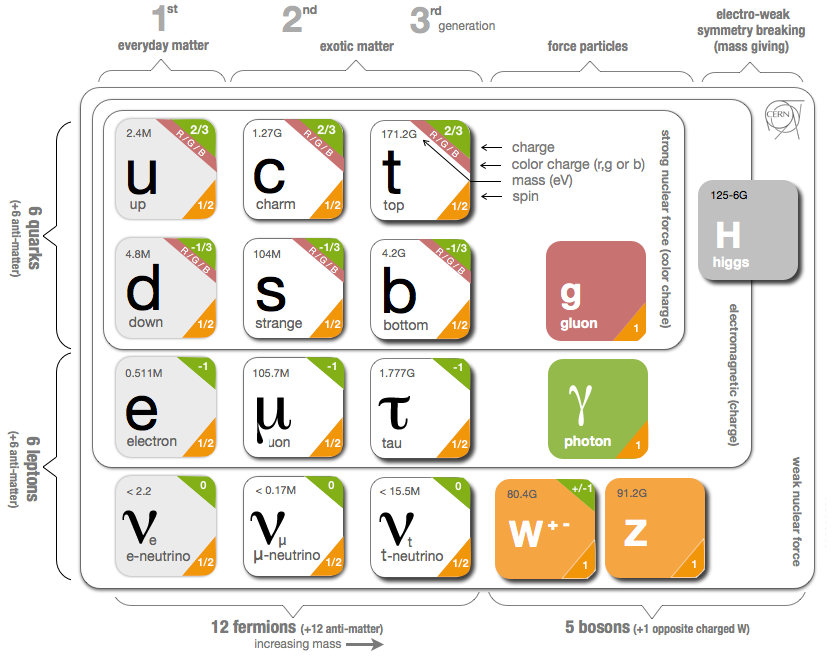
\includegraphics[scale=0.25]{figs/sm}
		\end{minipage}	
	\end{multicols}
\end{frame}

\begin{frame}{The Higgs Boson}
	\footnotesize
	\begin{multicols}{2}
		\begin{itemize}
		\justifying
			\item In Physics symmetry is a strong basic property: the theory must be invariant under change of frame;
			\item Particle interactions rise due to symmetry in Quantum Physics. However, symmetry brings a trouble: particles should not have mass!
			\item This is a clear contrast to what we see in the nature (we have mass);
			\item Solution: a new particle which interacts with other particles (and itself) giving their mass. This particle is the Higgs boson observed in 2012:
			\begin{overpic}
				[scale=0.25]{figs/higgs_plot}
				\put(25,50){\color{red}\small Higgs}
			\end{overpic}
			\item The Higgs can appear through some interactions of the elementary particles, such as:
		\end{itemize}
	\end{multicols}
	\vspace{0.2cm}
	\begin{multicols}{4}
		\begin{overpic}
			[scale=0.04]{figs/ggh_diagram}
			\put(20,87){$gg \rightarrow H$}
			\put(10,-17){fusion of gluons}
		\end{overpic}
		\begin{overpic}
			[scale=0.04]{figs/vbf_diagram}
			\put(15,90){$q\bar{q} \rightarrow Hq\bar{q}$}
			\put(-10,-17){fusion of bosons Z/W}
			\put(30,-30){(VBF)}
		\end{overpic}
		\begin{overpic}		
			[scale=0.04]{figs/vh_diagram}
			\put(15,105){$q\bar{q} \rightarrow VH$}
			\put(-10,-17){radiation from Z/W}
		\end{overpic}
		\begin{overpic}		
			[scale=0.04]{figs/tth_diagram}
			\put(20,90){$gg \rightarrow t\bar{t}H$}
			\put(-10,-15){fusion of top quarks}
		\end{overpic}								
	\end{multicols}
\end{frame}

\begin{frame}{Physics Processes in this Analysis}
	\begin{multicols}{2}
		\begin{minipage}{9cm}
			\begin{itemize}
		\justifying
				\item Search for Higgs produced via Vector Boson Fusion (VBF):
				\begin{itemize}
		\justifying
					\item second largest Higgs production mode;
					\item tree-level and clean of beyond-SM processes;
					\item good frame for measurements of Higgs properties;
					\item based on reconstruction of four isolated leptons + at least two jets;
				\end{itemize}
			\end{itemize}
		\end{minipage}
		\flushright
		\begin{minipage}{2.8cm}
			\begin{varblock}[2.8cm]{\center VBF - Signal}
				\begin{figure}
					\subfloat[$q\bar{q} \rightarrow Hq\bar{q}$]{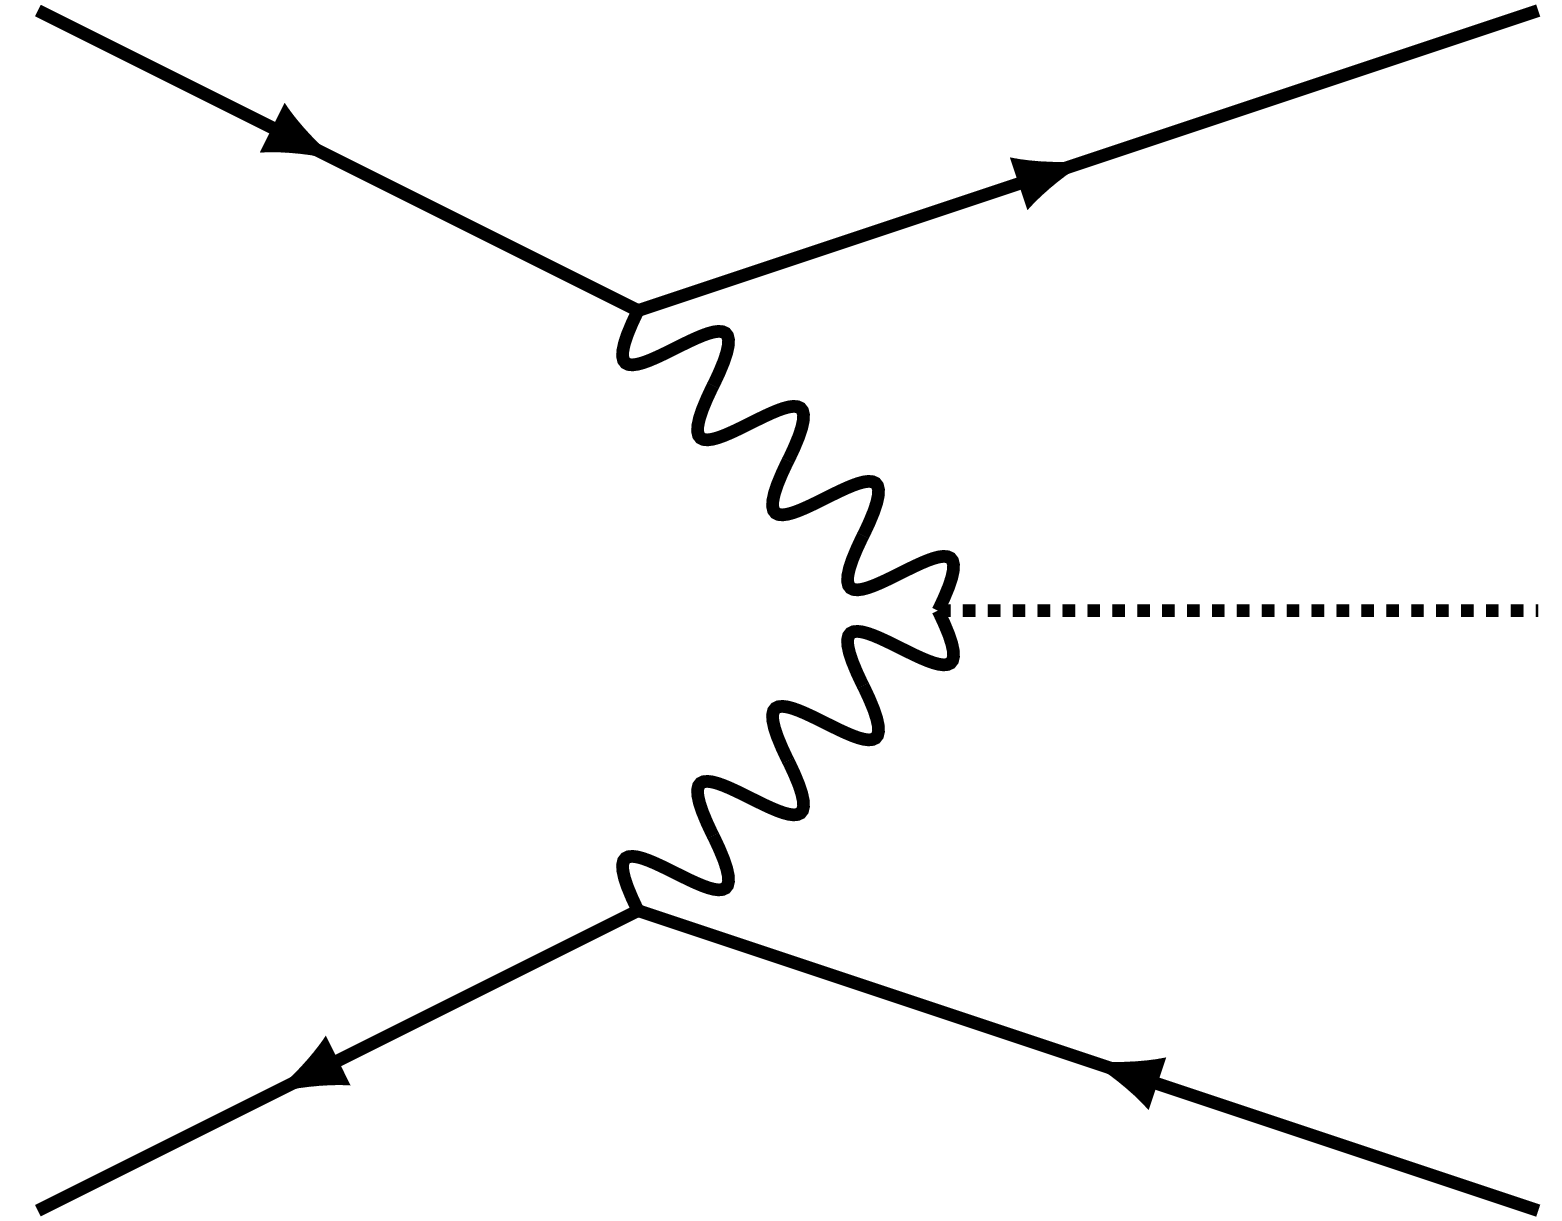
\includegraphics[scale=0.05,trim={0cm 0cm 0cm 1cm},clip]{figs/vbf_diagram}}
				\end{figure}
			\end{varblock}		
		\end{minipage}		
	\end{multicols}
	\vspace{-1cm}
	\begin{itemize}
		\justifying
		\item Expected backgrounds:
	\end{itemize}
	\begin{multicols}{2}
		\begin{varblock}[6.5cm]{\center SM Higgs Production Modes - Backgrounds}
			\begin{figure}
				\subfloat[$gg \rightarrow H$]{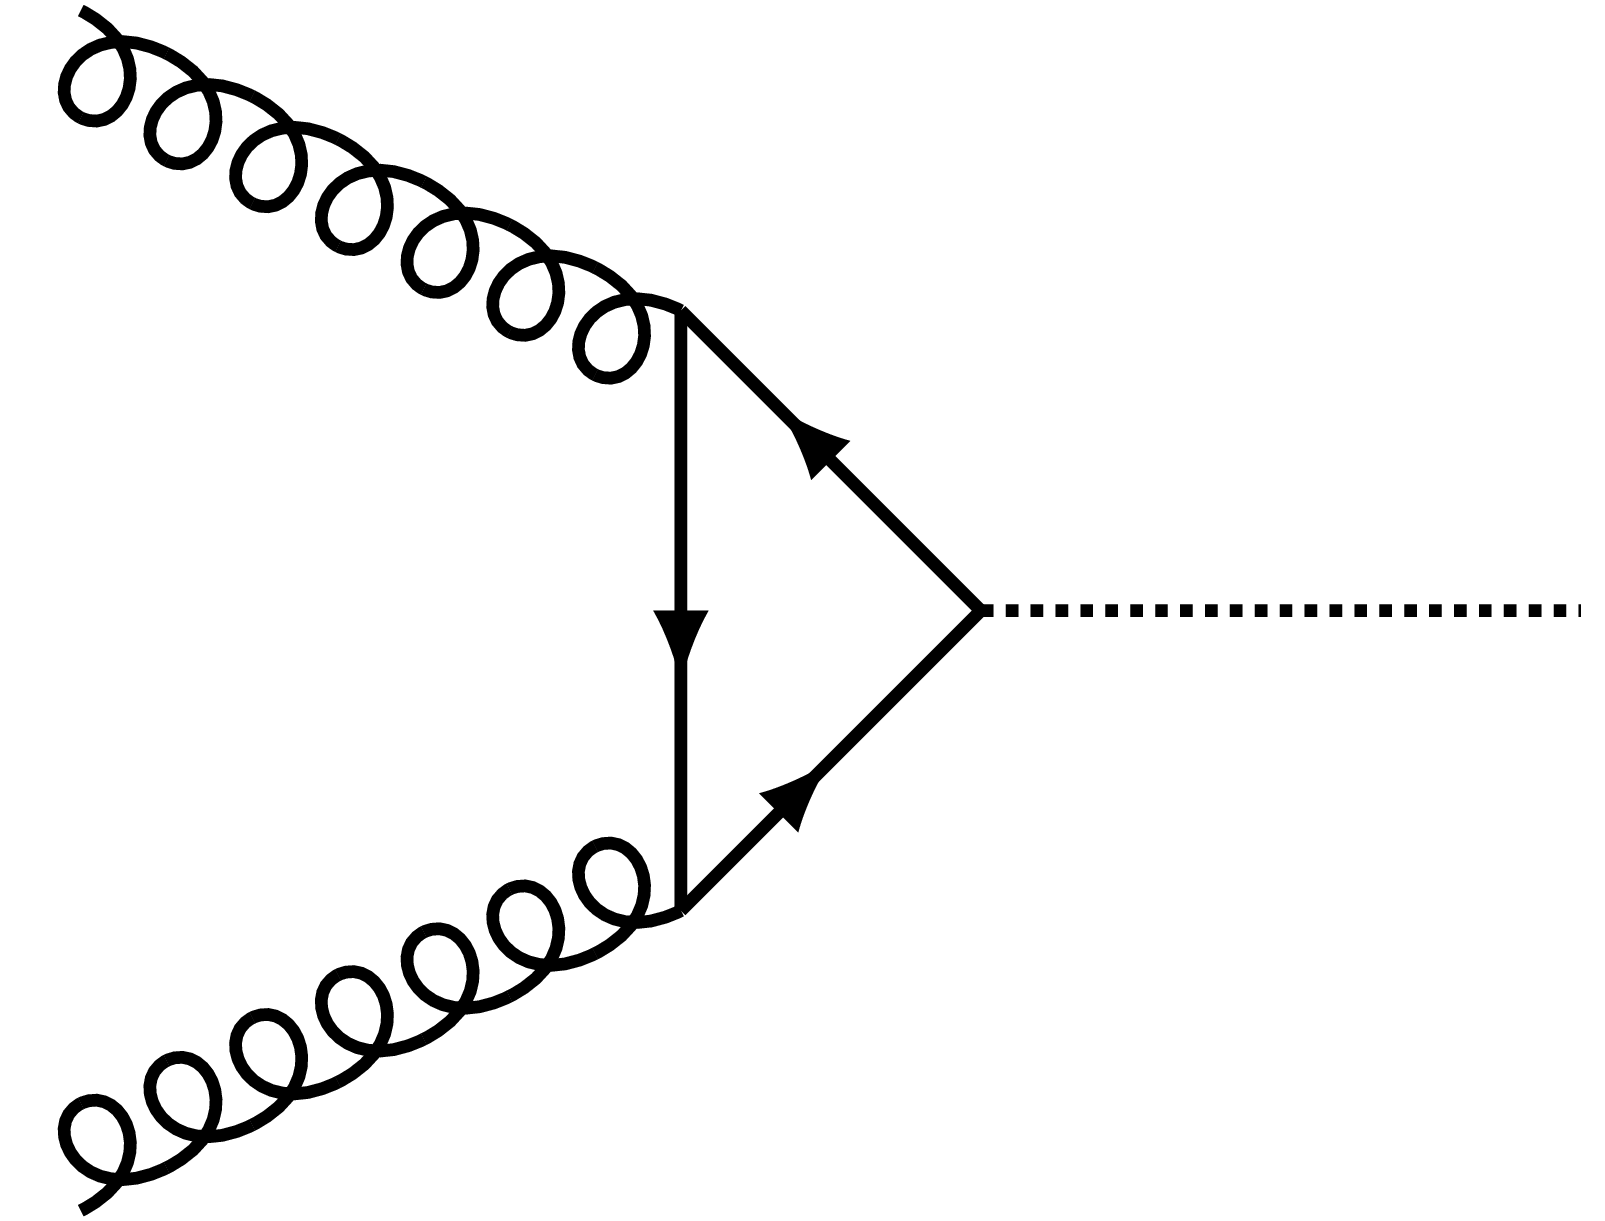
\includegraphics[scale=0.04]{figs/ggh_diagram}}
				\subfloat[$q\bar{q} \rightarrow VH$]{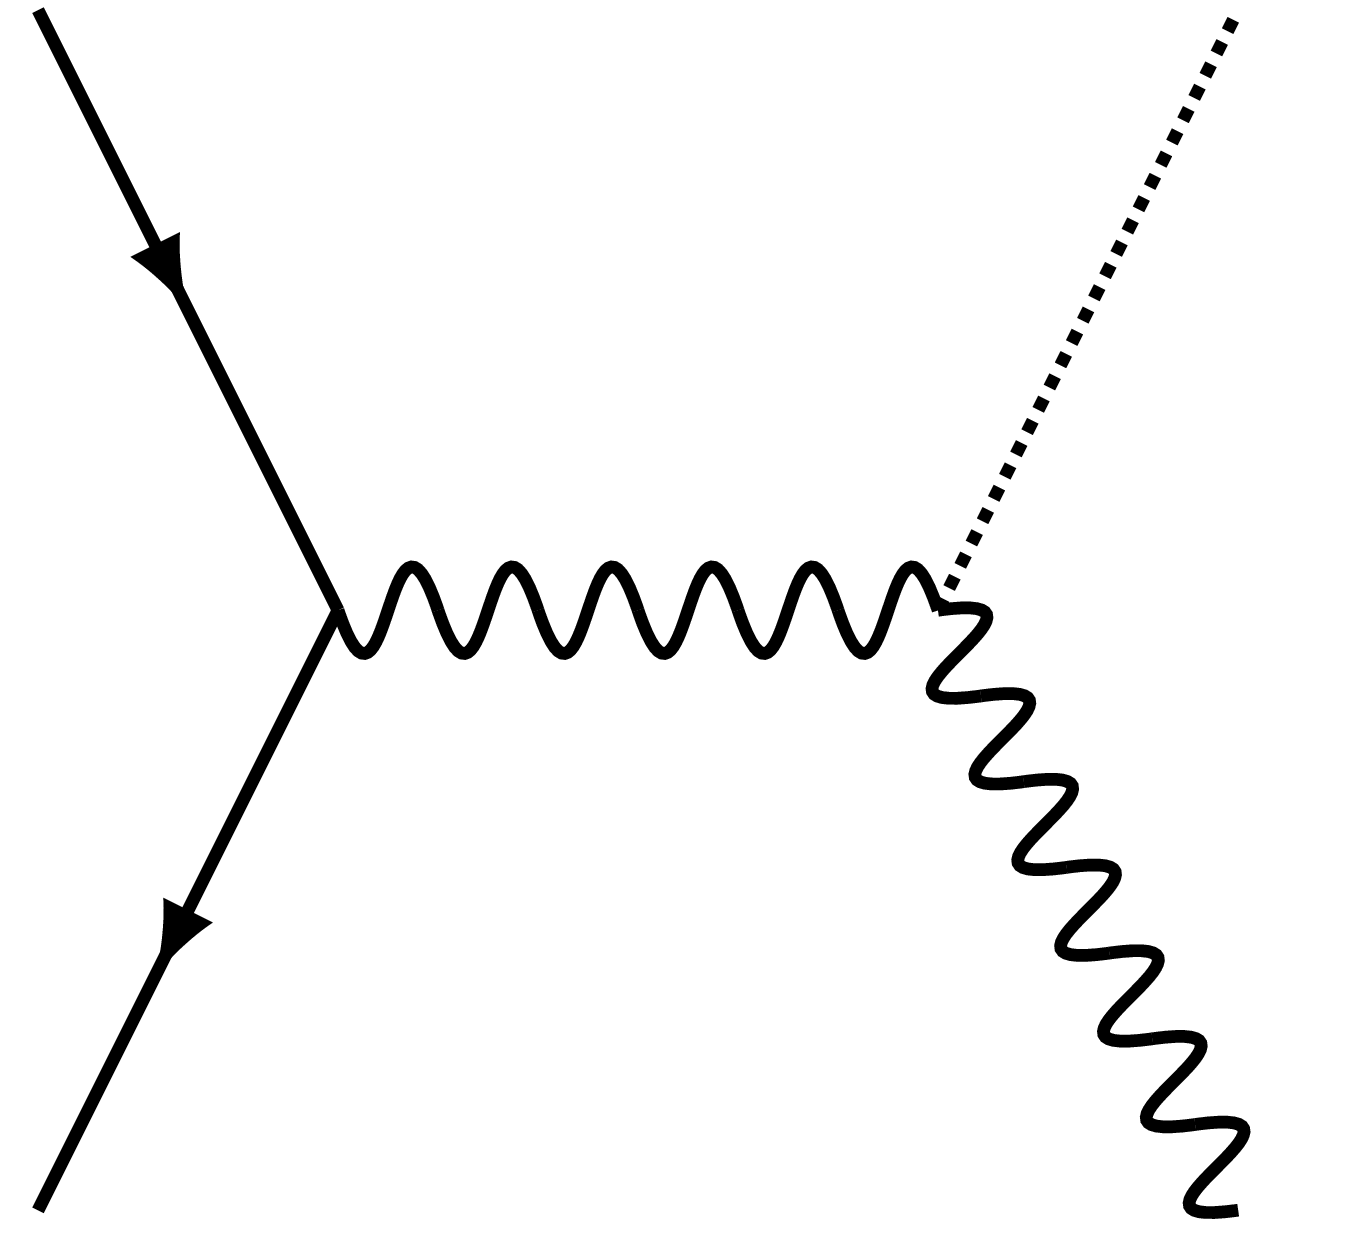
\includegraphics[scale=0.04]{figs/vh_diagram}}
				\subfloat[$gg \rightarrow t\bar{t}H$]{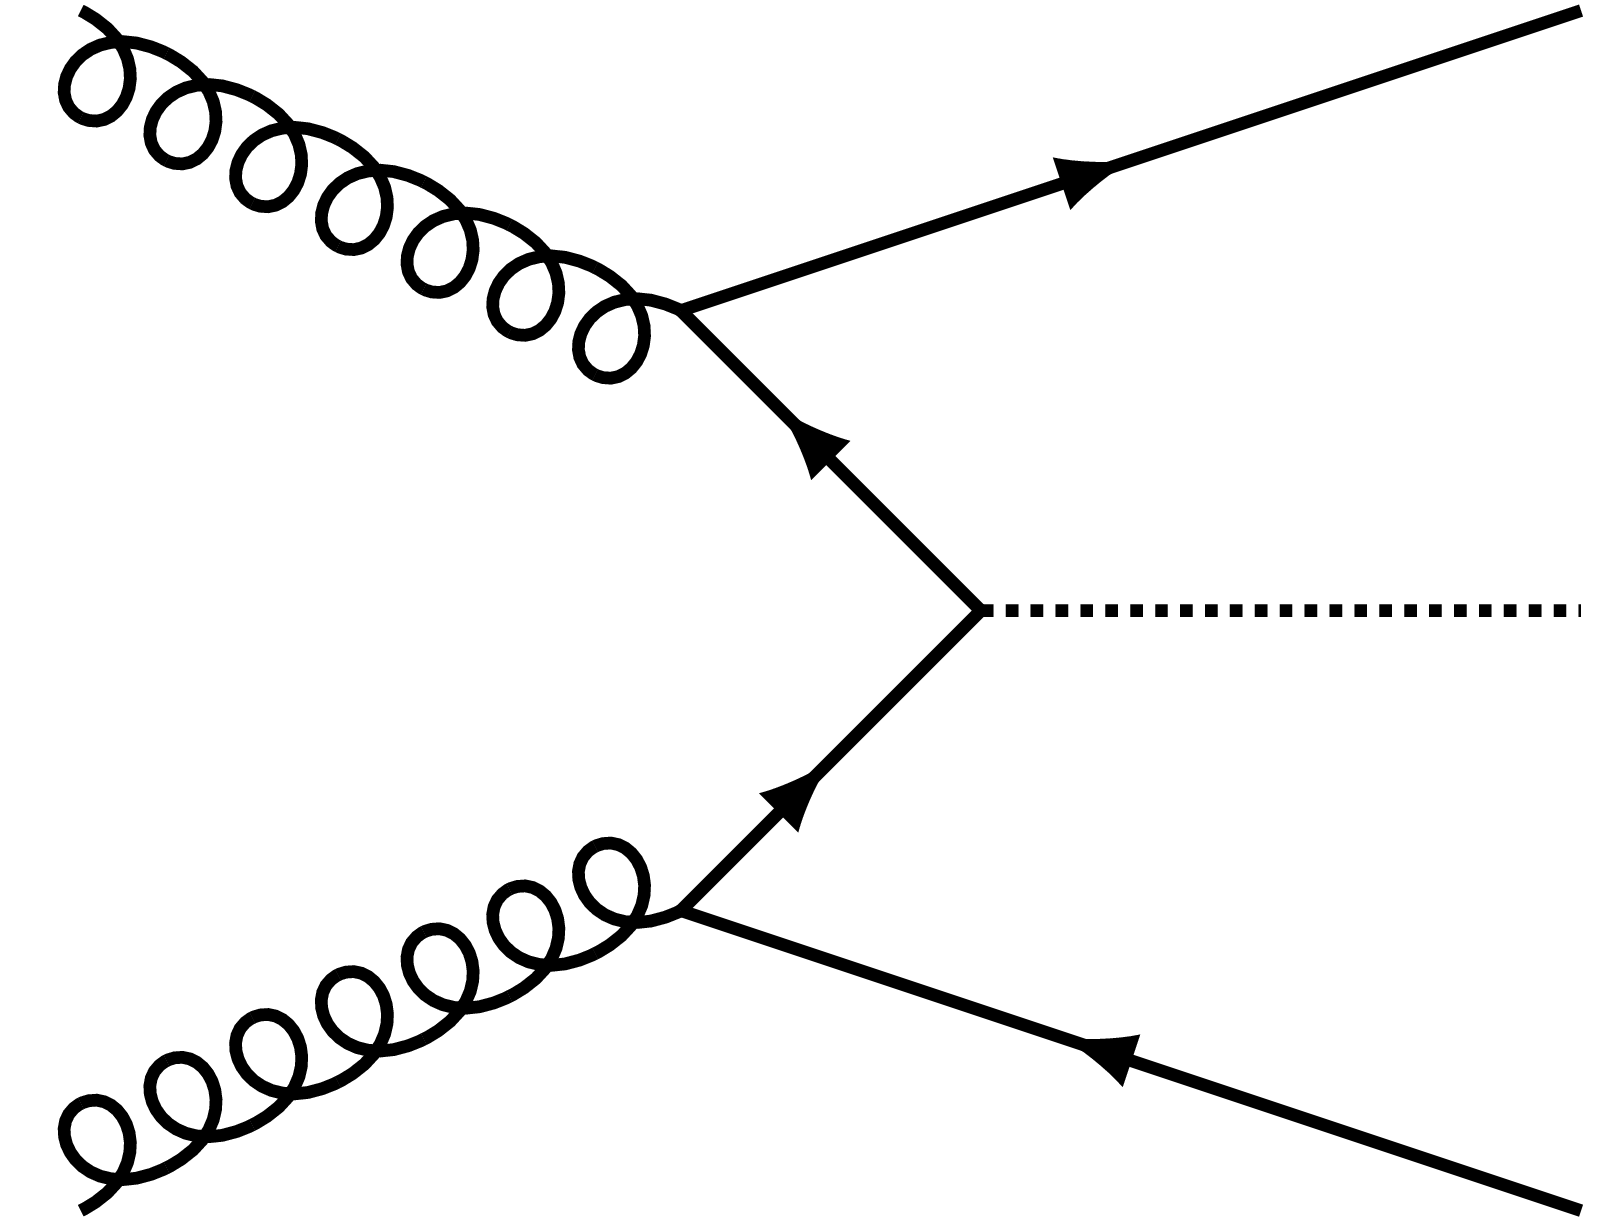
\includegraphics[scale=0.04]{figs/tth_diagram}}
			\end{figure}
		\end{varblock}
		\flushright
		\begin{minipage}{4.5cm}
			\vspace{-0.2cm}   		
			\begin{varblock}[4.5cm]{\center SM Backgrounds}
				\begin{figure}
					\subfloat[$q\bar{q} \rightarrow ZZ$]{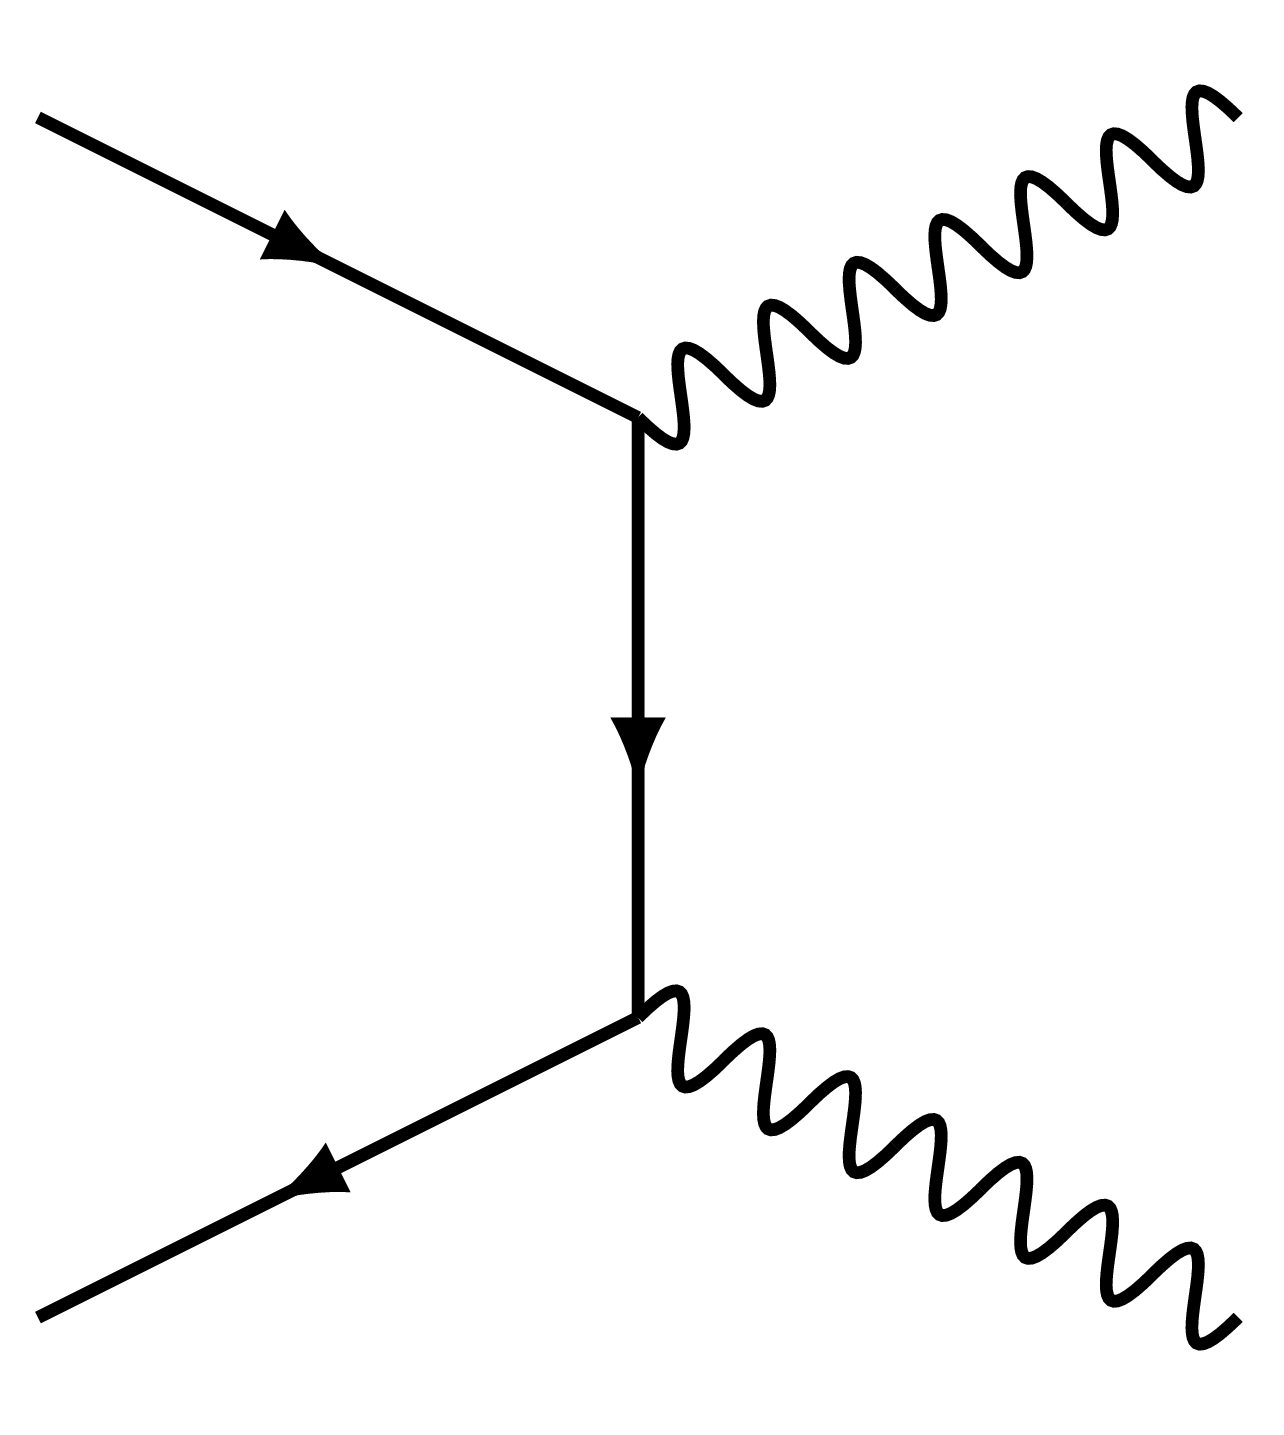
\includegraphics[scale=0.04,trim={0cm 3cm 0cm 4cm},clip]{figs/qqzz_diagram}}
					\subfloat[$gg \rightarrow ZZ$]{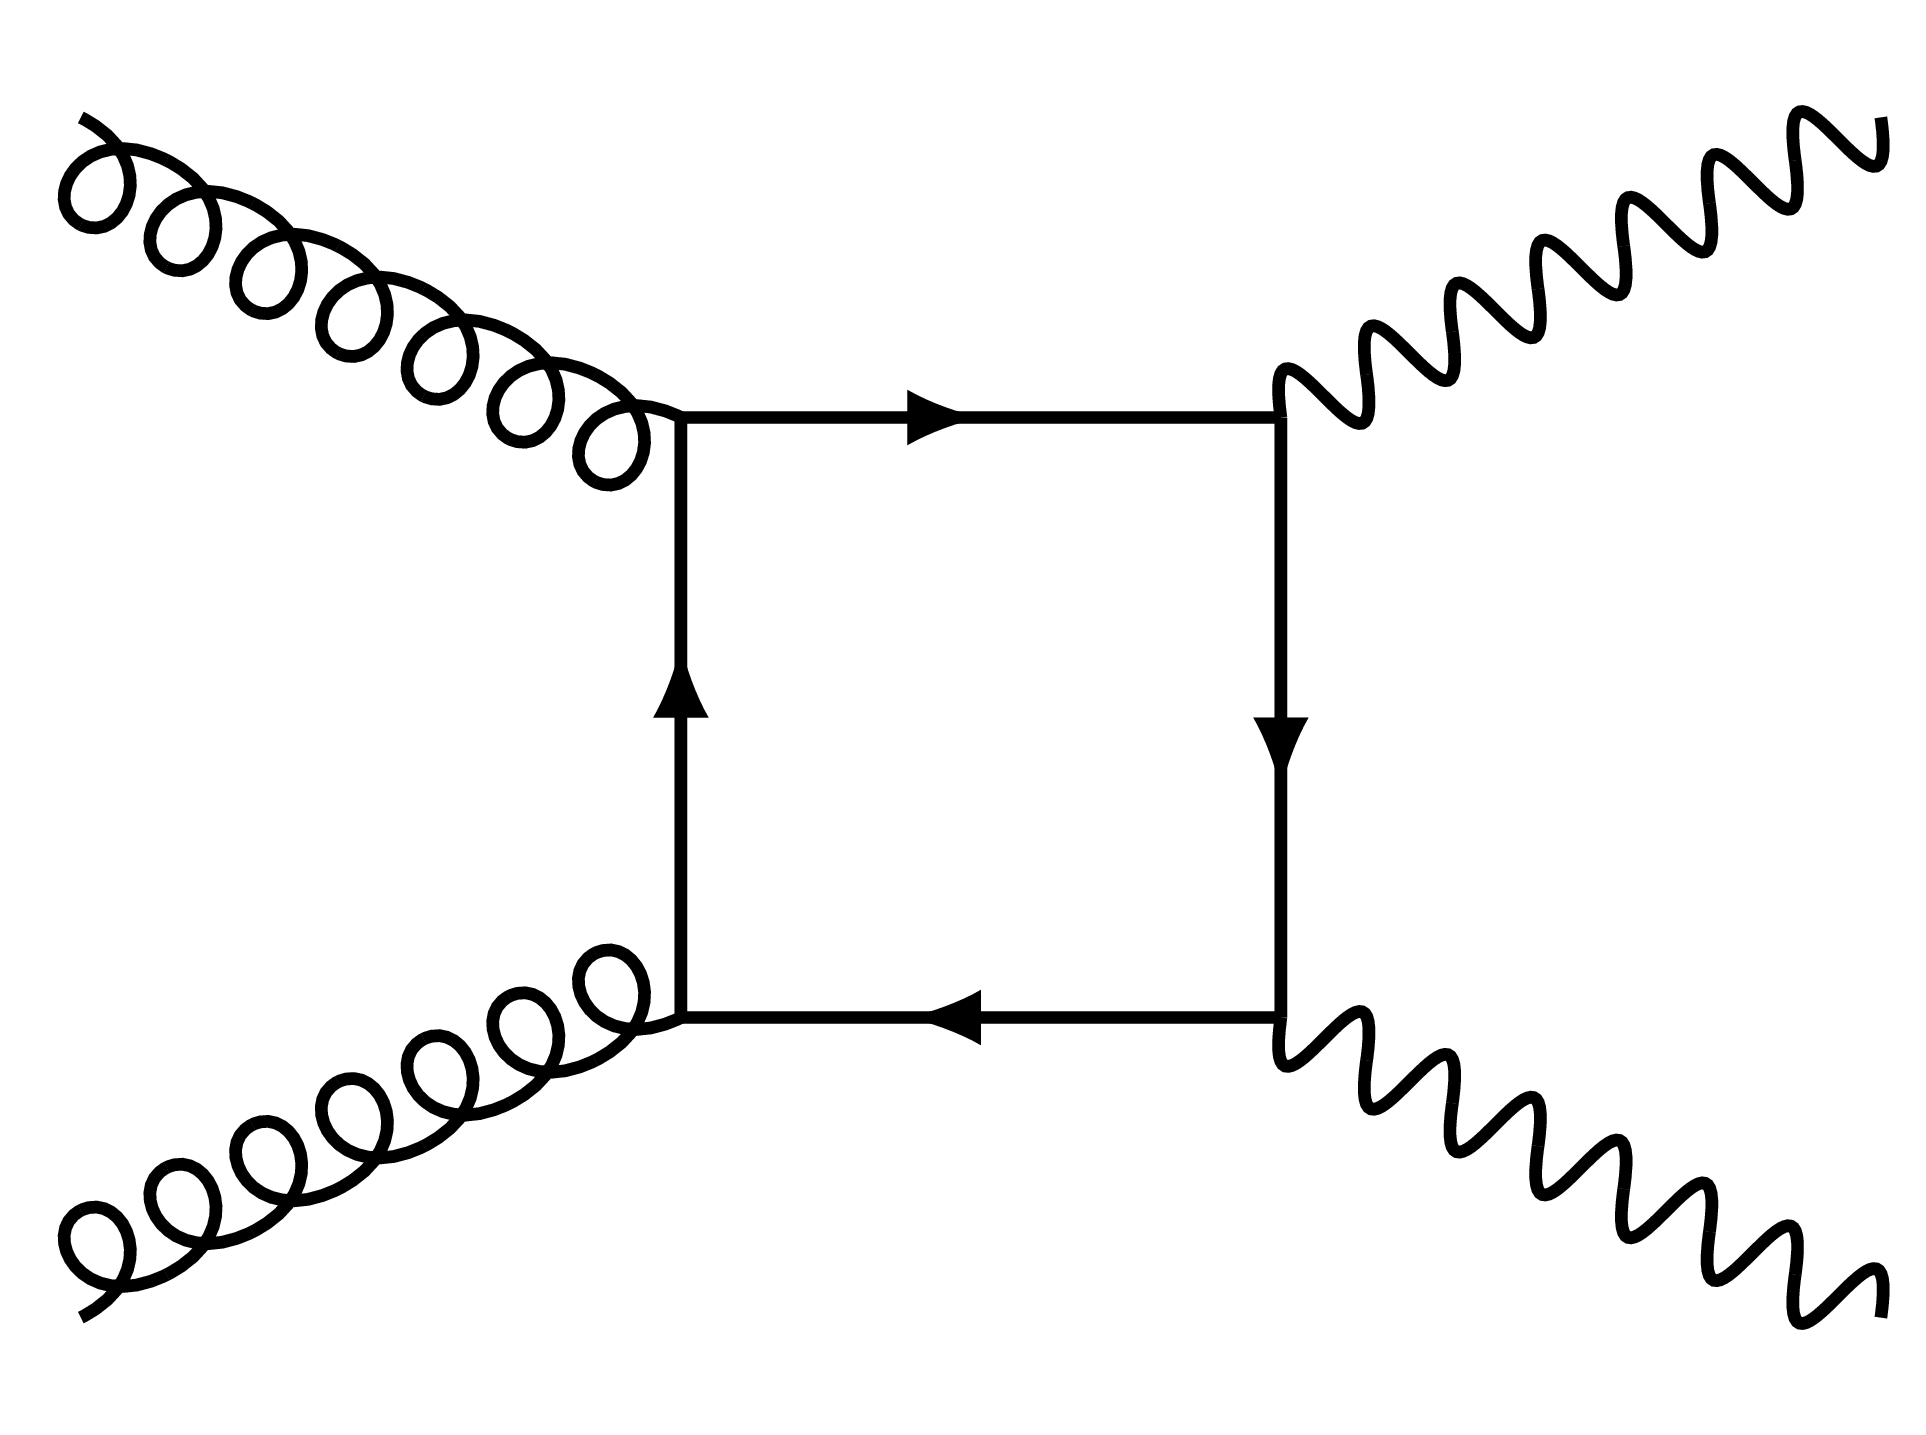
\includegraphics[scale=0.04,trim={0cm 3cm 0cm 4cm},clip]{figs/ggzz_diagram}}
				\end{figure}
			\end{varblock}
		\end{minipage}   	
	\end{multicols}
	\begin{itemize}
		\justifying
		\item Additionally there is the $Z+X$ derived via \textit{data-driven} method;
	\end{itemize}   	
\end{frame}

\subsection{The CMS Experiment at CERN}
\begin{frame}{{\color{blue}C}ompact {\color{blue}M}uon {\color{blue}S}olenoid in a Nutshell}
	\vspace{-0.5cm}
	\begin{multicols}{2}
		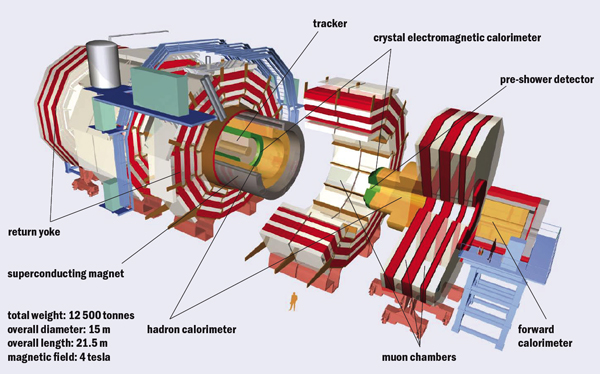
\includegraphics[width=8.6cm,height=5.2cm]{figs/cms_scheme}\\
		\flushright
		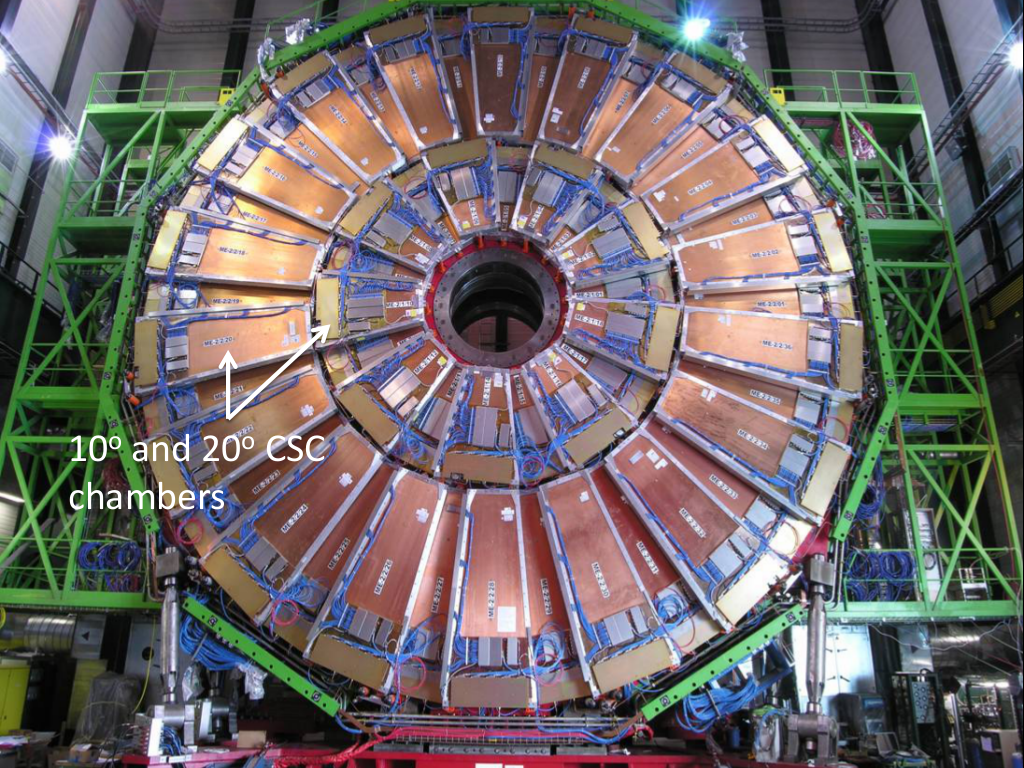
\includegraphics[width=3.3cm,height=2.6cm]{figs/muon_csc_dt}\\
		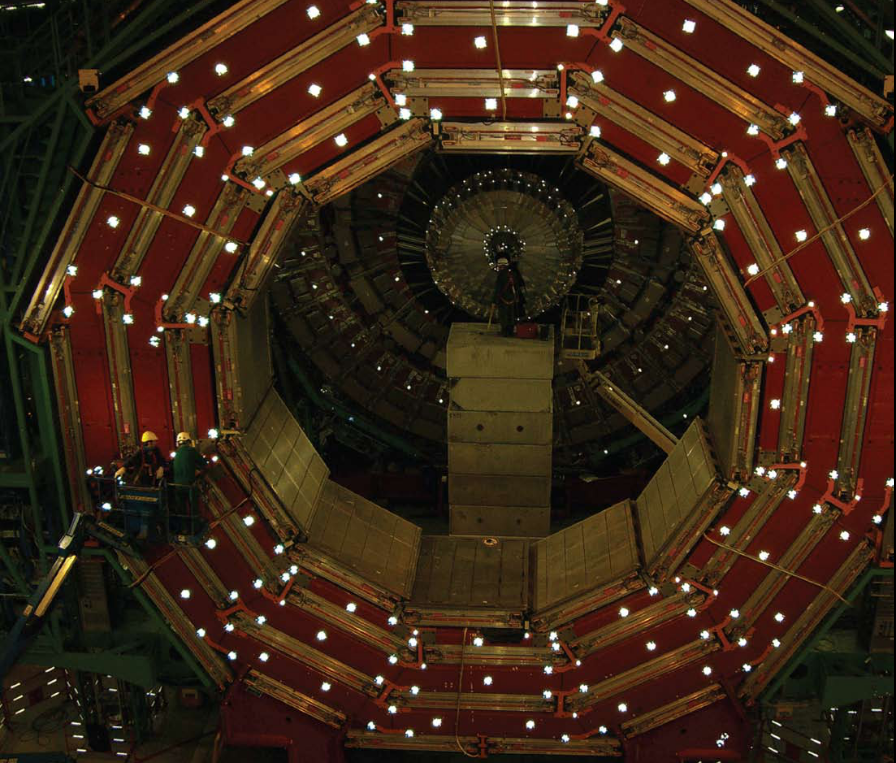
\includegraphics[width=3.3cm,height=2.6cm]{figs/muon_barrel}
	\end{multicols}
	\vspace{-0.3cm}
	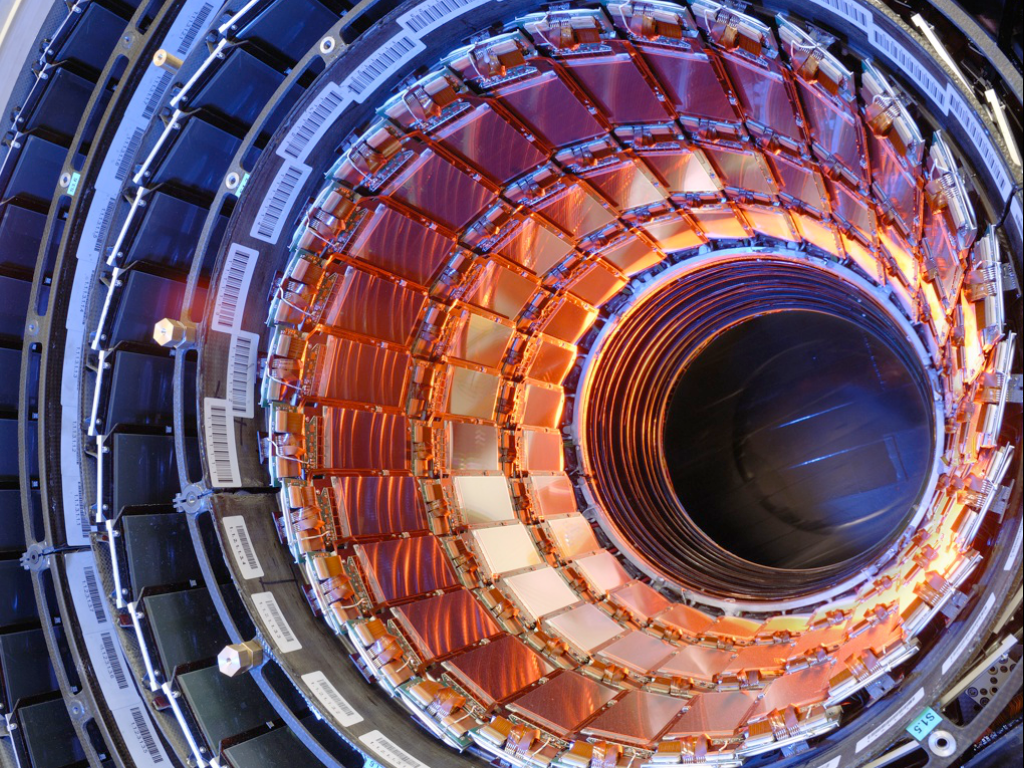
\includegraphics[width=3.83cm,height=2.7cm]{figs/strip_tracker}\quad
	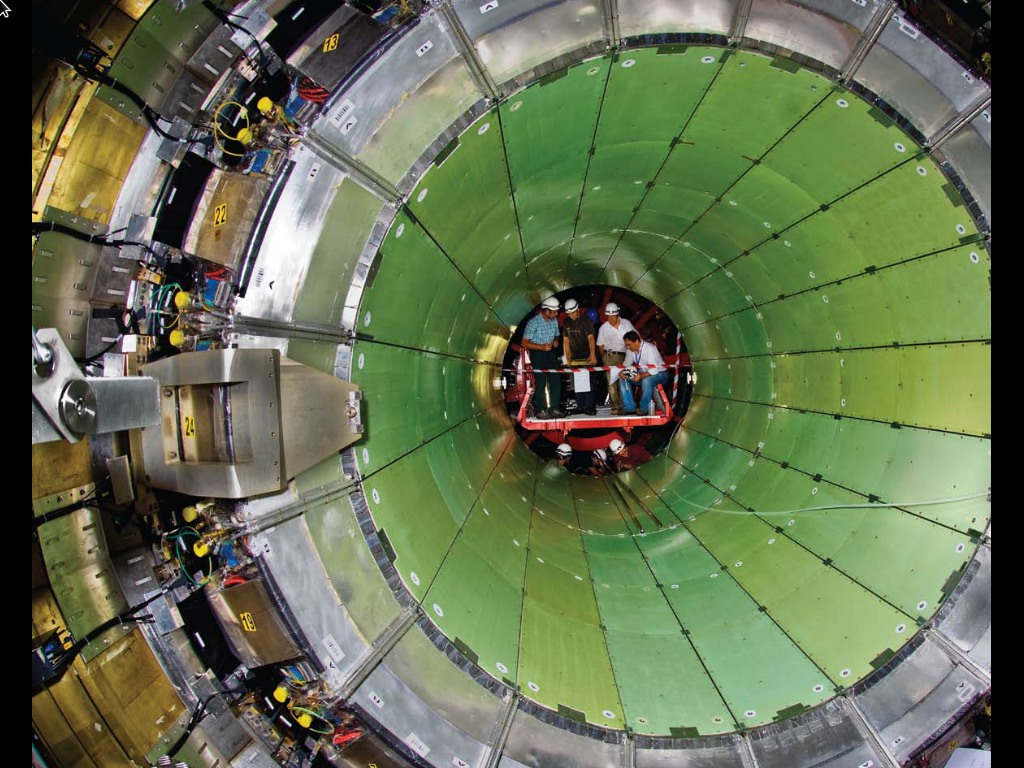
\includegraphics[width=3.83cm,height=2.7cm]{figs/ecal_mont}\quad
	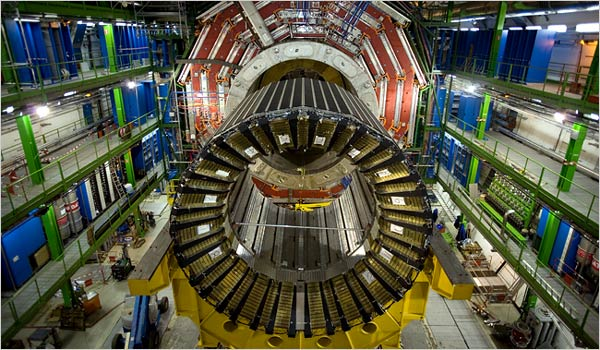
\includegraphics[width=3.83cm,height=2.7cm]{figs/cms_hcal}
\end{frame}

\begin{frame}{CMS-Particles Interaction Profile}
	\center
	\begin{overpic}
		[scale=0.3]{figs/cms_deteccao}
		\put(30,51){Particles Profiles through CMS Detector}
	\end{overpic}
	\begin{itemize}
		\justifying
		\item CMS has particle-specialized sub-detectors;
		\item "Long-life" particles (reach detectors) are identified by patterns from the sub-detectors;
		\item "Short-life" particles (decay into other particles before reach a detector) are accessed through the properties of "long-life" particles;
	\end{itemize}	
\end{frame}

\subsection{Datasets, Triggers and Simulated Samples}
\begin{frame}{Datasets and Triggers}
	\begin{itemize}
		\justifying
		\item Data:
		\begin{itemize}
		\justifying
			\item full 2016 Data: L = 35.9fb$^{-1}$, 03Feb ReReco (full list in backup);
			\item JSON: Cert\_271036\_284044\_13TeV\_23Sep2016ReReco\_Collisions16\_JSON.txt.
		\end{itemize}
		\item Triggers:
		\begin{itemize}
		\justifying
			\item based on multi-lepton HLT paths;
			\item isolated di-lepton paths + non-isolated tri-lepton paths + single-lepton paths;
			\item requirements to avoid double-counting is applied;
			\item overall trigger efficiency is higher than 99$\%$ wrt. 4-lepton analysis selection;
		\end{itemize}
	\end{itemize}
	\centering
	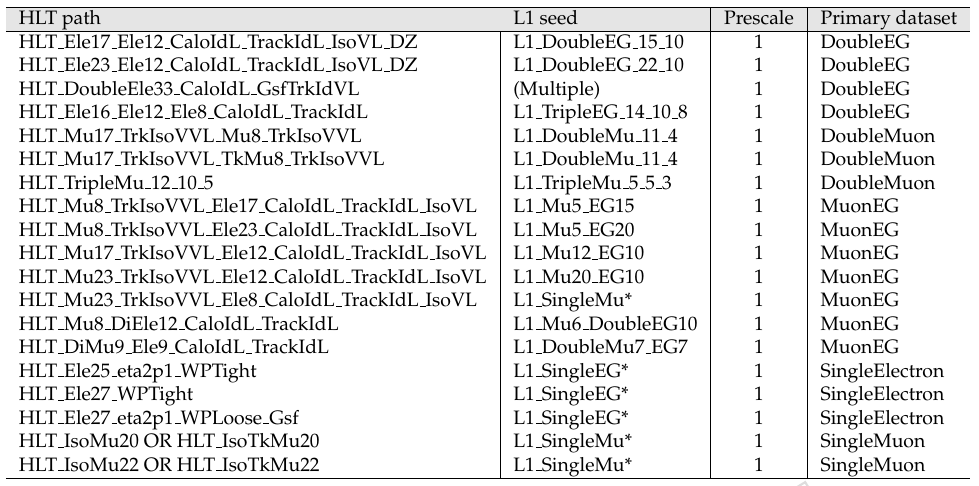
\includegraphics[scale=0.4]{figs/trigger_paths}
\end{frame}

\begin{frame}{Simulated Samples}
	\begin{itemize}
		\justifying
		\footnotesize
		\item Signal: VBF\_HToZZTo4L\_M125\_13TeV\_powheg2\_JHUgenV6\_pythia8;
		\item Background: remaining samples in the table;
		\item Special samples for ggH ({\color{blue}*}) and qqZZ ({\color{blue}**}) included.
	\end{itemize}
	\centering
	\begin{overpic}
		[scale=0.5]{figs/simulated_samples}
		\put(0,61){\color{blue}*}
		\put(-1,32){\color{blue}**}
	\end{overpic}
\end{frame}

\subsection{Objects Selections}
\begin{frame}{Objects Selections}
	\begin{block}{\center Electrons (momentum callibration applied)}
		\hspace{0.35cm}
		\begin{minipage}{9cm}
		\begin{multicols}{2}
			\begin{varblock}[4cm]{\center Loose}
				\begin{itemize}
		\justifying
					\item $p_{T} > 7$ GeV;
					\item $|\eta| < 2.5$;
					\item $|d_{xy}| < 0.5$ cm;
					\item $|d_{z}| < 1.0$ cm.
				\end{itemize}				
			\end{varblock}
			\begin{varblock}[6.5cm]{\center Tight}
				\begin{itemize}
		\justifying
					\item Loose selections plus:
					\begin{itemize}
		\justifying
						\item $|SIP_{3D}| < 4.0$;
						\item Isolation ($\Delta R = 0.3$) < 0.35;
						\item MVA (BDT) calorimeter-based:
					\end{itemize}
				\end{itemize}
				\centering
				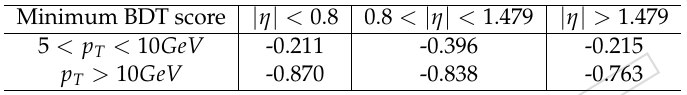
\includegraphics[scale=0.35]{figs/electron_bdt}
			\end{varblock}
		\end{multicols}
	\end{minipage}
	\end{block}
	\begin{block}{\center Muons (momentum callibration and FSR applied)}
		\hspace{0.35cm}
		\begin{minipage}{9cm}
			\begin{multicols}{2}
				\begin{varblock}[4cm]{\center Loose}
					\begin{itemize}
		\justifying
						\item Global/Tracker Muons;
						\item $p_{T} > 5$ GeV;
						\item $|\eta| < 2.4$;
						\item $|d_{xy}| < 0.5$ cm;
						\item $|d_{z}| < 1.0$ cm.
					\end{itemize}
				\end{varblock}
				\begin{varblock}[6.5cm]{\center Tight}
					\begin{itemize}
		\justifying
						\item Loose selections plus:
						\begin{itemize}
		\justifying
							\item PF Muon;
							\item $|SIP_{3D}| < 4.0$;
							\item Isolation ($\Delta R = 0.3$) < 0.35;
							\item Ghost-cleaning (single-$\mu$ as more).
						\end{itemize}
					\end{itemize}				
				\end{varblock}
			\end{multicols}
		\end{minipage}
	\end{block}	
\end{frame}

\begin{frame}{Objects Selections}
	\begin{block}{\center Photons and FSR}
		\begin{itemize}
		\justifying
			\item $p_{T} > 2$ GeV, $|\eta| < 2.4$;
			\item Isolation ($\Delta R = 0.3$) < 1.8;
			\item $\Delta R (\gamma,l)/E_{T,\gamma}^{2} \geq 0.012$ and $\Delta R (\gamma,l) \geq 0.5$;
		\end{itemize}
	\end{block}
	\begin{block}{\center Jets (JECs applied)}
		\begin{itemize}
		\justifying
			\item anti-kT (R = 0.4) PF CHS (\textit{Carged Hadron Subtracted}) jets;
			\item $p_{T} > 30$ GeV, $|\eta| < 4.7$;
			\item cleaning $\Delta R(jet,l/\gamma) > 0.4$;
			\item b-tagging with CSV (\textit{Combined Secondary Vertex}) algorithm;
		\end{itemize}
	\end{block}	
	\begin{block}{\center MET (\textit{Missing Transverse Energy})}
		\begin{itemize}
		\justifying
			\item PF MET with type-1 correction:
			$\vec{E}_{T}^{miss} = - ( \sum_{jets} \vec{p}_{T}^{JEC} + \sum_{uncl.} \vec{p}_{T} )$;
			\item filters\footnote{See backup slides.} from JETMET POG applied (improves signal-to-noise ratio).
		\end{itemize}
	\end{block}	
\end{frame}

\subsection{Event Selections}
\begin{frame}{Event Selections}
	\begin{block}{\center SM Higgs}
		\begin{itemize}
		\justifying
			\item[1] \textbf{Z candidates}: pair of same-flavor, opposite-charge and FSR corrected leptons ($e^{+}e^{-}$, $\mu^{+}\mu^{-}$) having invariant mass $12 < m_{ll(\gamma)} < 120$ GeV;
			\item[2] \textbf{ZZ candidates}: pair of non-overlapping (different leptons) Z candidates. The Z with smallest $|m_{ll(\gamma)}-m_{Z}^{PDG}|$ is identified as $Z_{1}$ and the other Z as $Z_{2}$. ZZ candidates must satisfy:
			\begin{itemize}
		\justifying
				\item any two leptons must have $\Delta R(\eta,\phi) > 0.02$ (\textbf{ghost removal});
				\item at least two out of the four leptons must have $p_{T} >$ 10 and 20 GeV;
				\item any two leptons must have (without FSR-$\gamma$) $m_{ll} >$ 4 GeV (\textbf{QCD suppression});
				\item $m_{Z_{1}} >$ 40 GeV and $m_{Z_{1}Z_{2}} >$ 100 GeV;
				\item if more than one ZZ candidate survives previous cuts, the one with highest scalar leptons $p_{T}$ sum is chosen;
			\end{itemize}
		\end{itemize}
	\end{block}
	\centering {\huge \textbf{+}}
	\begin{block}{\center VBF Signal Region (VBF-SR)}
		\begin{itemize}
		\justifying
			\item[3] In order to enhance VBF-to-background ratio:
			\begin{itemize}
		\justifying
				\item Number of jets:
			\begin{itemize}
		\justifying
				\item EITHER, 2 or 3 jets from which at most one b-tagged jet;
				\item OR, more than 3 jets with no b-tagged jet;
			\end{itemize}
				\item ZZ candidates must have $118 \leq m_{Z_{1}Z_{2}} \leq 130$ GeV;
			\end{itemize}
		\end{itemize}
	\end{block}
\end{frame}

\subsection{Signal and Background Estimation}
\begin{frame}{Signal and Background Estimation}
	\begin{itemize}
		\justifying
		\item In this analysis the background at the VBF-SR is composed by:
		\begin{itemize}
		\justifying
			\item remaining Higgs production modes ($ggH$, $VH$ and $ttH$);
			\item SM backgrounds ($qqZZ$, $ggZZ$ and $Z+X$);
		\end{itemize}
		\item The Higgs production modes (including VBF) are estimated from MC normalized by proper $\sigma.BR$ given by LHC Higgs XS Working Group computation;
		\item The SM backgrounds $qqZZ$ and $ggZZ$ are modeled from MC and properly applying scale factors accounting for NLO and NNLO corrections, as done for the SM Higgs analysis;
		\item The SM background $Z+X$ is estimated from Data via the \textit{data-driven} Fake Rate (FR) method;
	\end{itemize}
\end{frame}

\begin{frame}{$Z+X$ Background Estimation}
	\begin{itemize}
		\justifying
		\item Originates from processes with non-prompt leptons: heavy-flavor meson decays, mis-reconstructed jets and electrons from $\gamma$ conversions;
		\item Strategy: measure FR in specific control regions (CRs) and apply it to the SR;
		\item {\color{red}First step}, measuring the FR:
		\begin{itemize}
		\justifying
			\item samples of $Z_{l_{1}l_{2}}+l_{3}$ ($l_{1,2}$ \textit{tight} leptons, $l_{3}$ \textit{loose} lepton);
			\item $p_{T}^{l_{1},l_{2}} >$ 10, 20 GeV, $m_{l_{1}l_{2}} <$ 4 GeV, $|m_{l_{1}l_{2}}-m_{Z}^{PDG}| <$ 7 GeV and $E_{T}^{miss} <$ 25 GeV;
			\item contribution from $WZ$ (with potential 3 real leptons) is subtracted;
		\end{itemize}
		\item The FR ($N_{tight}/N_{loose}$, ie. probability of \textit{loose} lepton pass \textit{tight} selections) is mapped wrt. to $p_{T}^{l_{3}}$ vs. $\eta^{l_{3}}$:
	\end{itemize}
	\centering
	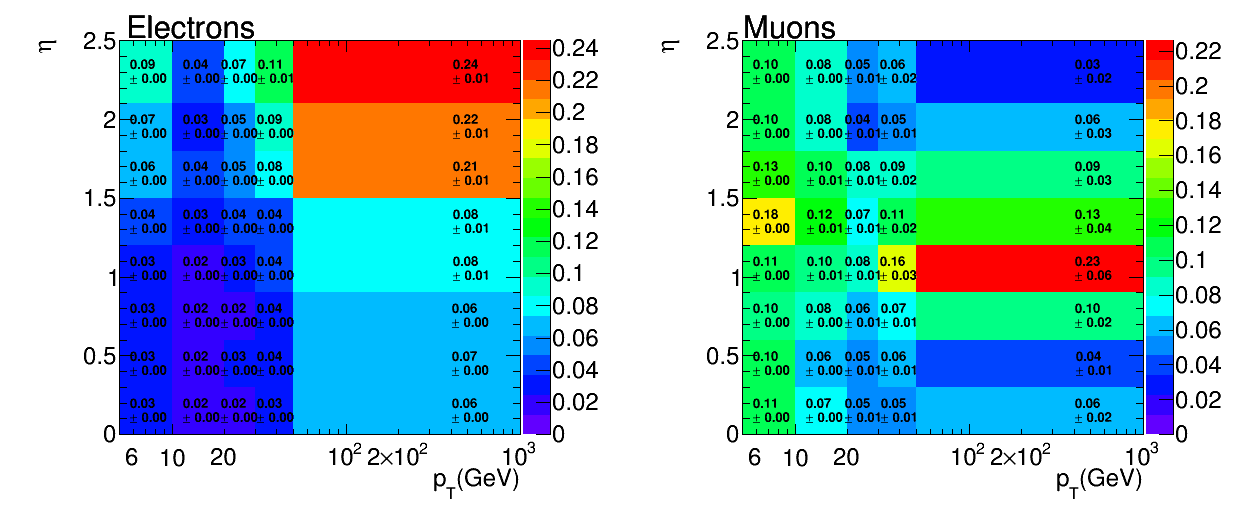
\includegraphics[scale=0.28]{figs/fake_rate_2D_maps_corrected}
\end{frame}

\begin{frame}{$Z+X$ Background Estimation}
	\begin{itemize}
		\justifying
		\item {\color{red}Second step}, building CRs:
		\begin{itemize}
		\justifying
			\item Orthogonal to the SM Higgs selections and enriched by fake-lepton events;
			\item Require $Z_{l_{1}l_{2}}Z_{l_{3}l_{4}}$ where $l_{1,2}$ are always \textit{tight} leptons and if $l_{3,4}$ are \textit{loose} leptons, define 2P2F while if only $l_{4}$ is \textit{loose}, define 3P1F;
		\end{itemize}
	\end{itemize}
	\vspace{-0.3cm}
	\begin{multicols}{2}
	\begin{varblock}[5.8cm]{\center 2P2F CR: $w_{Data} = \frac{f_{3}}{1-f_{3}}+\frac{f_{4}}{1-f_{4}}$}
		\begin{overpic}
			[scale=0.135,trim={1cm 0cm 2cm 1cm},clip]{figs/m4l_2p2f_4mu_smhiggs}
		\end{overpic}\hspace{-0.1cm}
		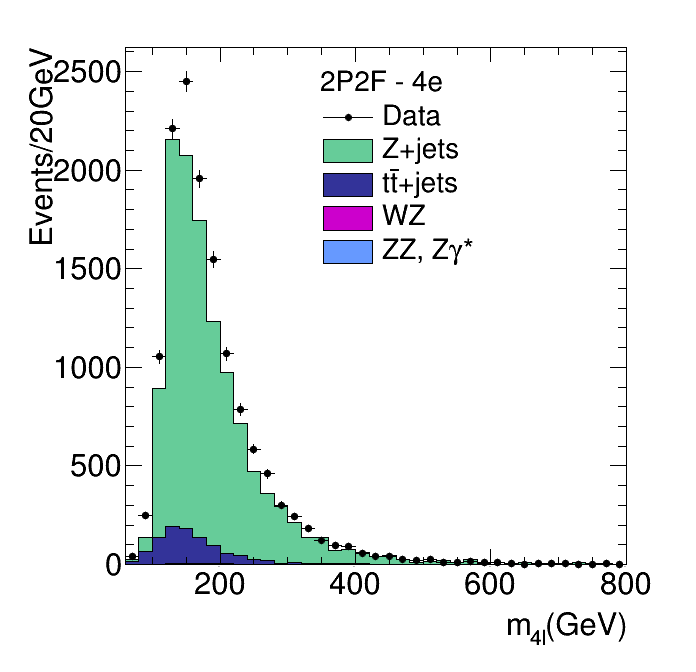
\includegraphics[scale=0.135,trim={1cm 0cm 2cm 1cm},clip]{figs/m4l_2p2f_4e_smhiggs}\\
		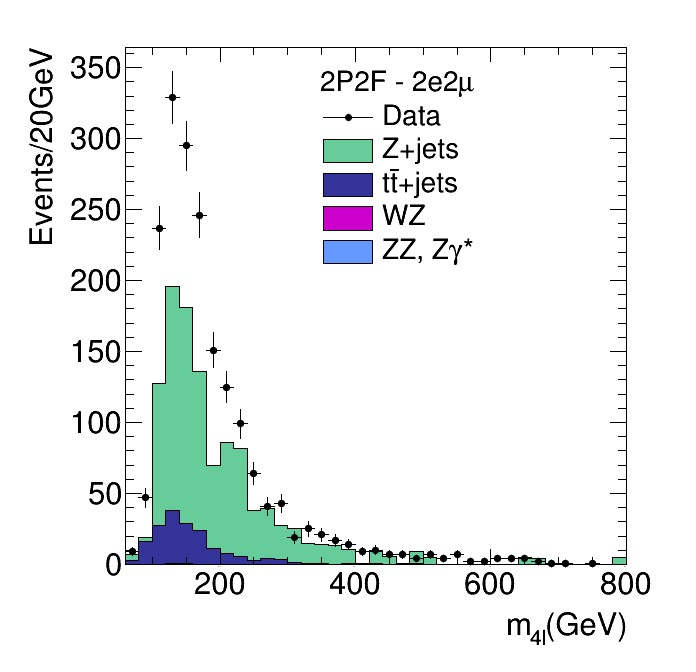
\includegraphics[scale=0.135,trim={1cm 0cm 2cm 1cm},clip]{figs/m4l_2p2f_2e2mu_smhiggs}
		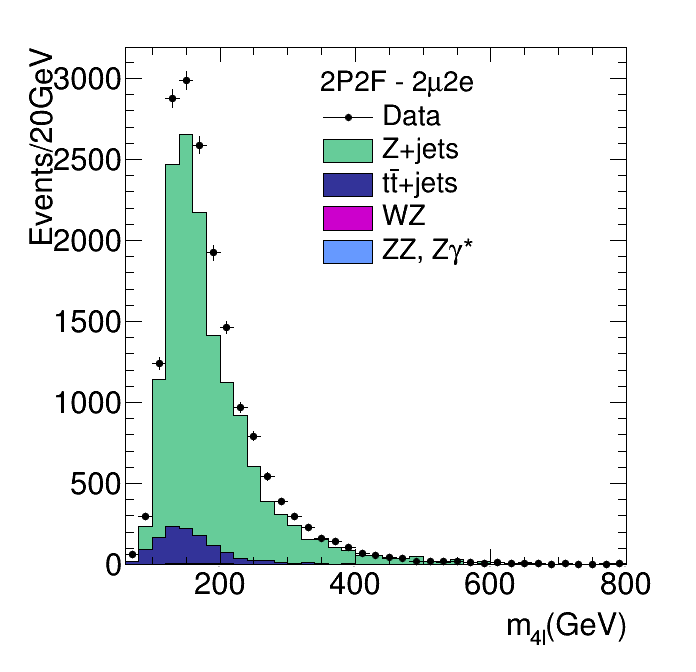
\includegraphics[scale=0.135,trim={1cm 0cm 2cm 1cm},clip]{figs/m4l_2p2f_2mu2e_smhiggs}		
	\end{varblock}	
	\begin{varblock}[5.8cm]{\center 3P1F CR: $w_{Data} = \frac{f_{4}}{1-f_{4}}$}
		\begin{overpic}
			[scale=0.135,trim={1cm 0cm 2cm 1cm},clip]{figs/m4l_3p1f_4mu_smhiggs}
		\end{overpic}\hspace{-0.1cm}
		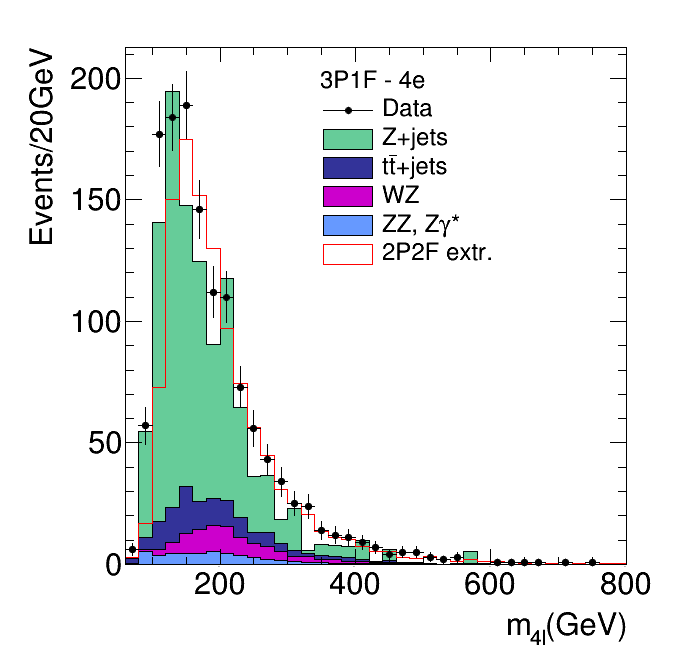
\includegraphics[scale=0.135,trim={1cm 0cm 2cm 1cm},clip]{figs/m4l_3p1f_4e_smhiggs}\\
		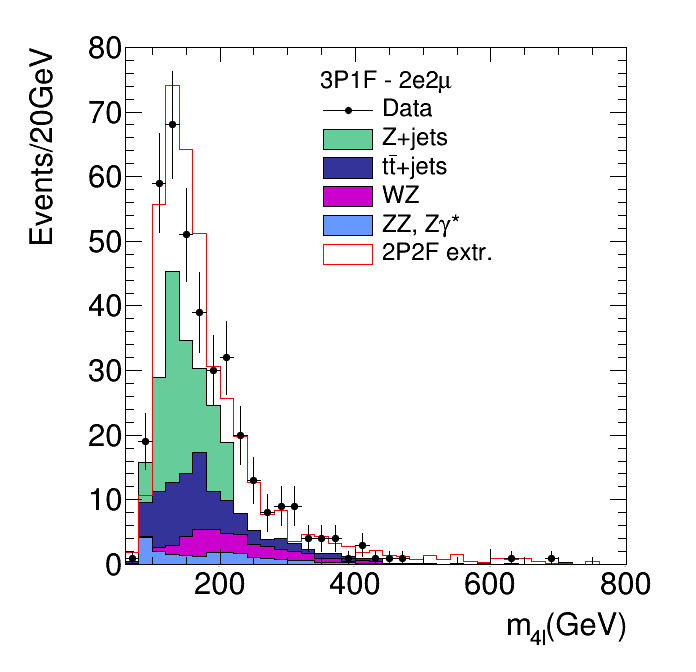
\includegraphics[scale=0.135,trim={1cm 0cm 2cm 1cm},clip]{figs/m4l_3p1f_2e2mu_smhiggs}
		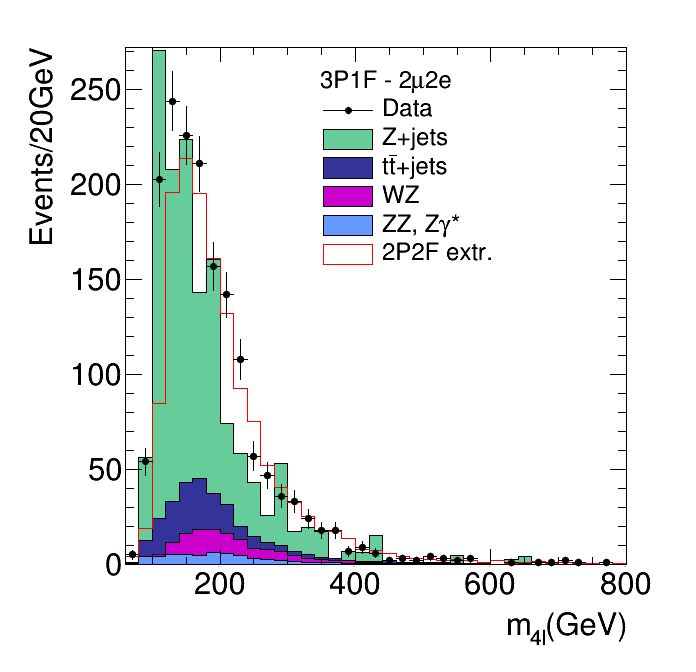
\includegraphics[scale=0.135,trim={1cm 0cm 2cm 1cm},clip]{figs/m4l_3p1f_2mu2e_smhiggs}		
	\end{varblock}		
	\end{multicols}	
\end{frame}

\begin{frame}{$Z+X$ Background Estimation}
	\begin{itemize}
		\justifying
		\item {\color{red}Third step}, using the measured FR($p_{T}$, $\eta$) in order to estimate $Z+X$ yield and shape in the SR;
		\item At SR, $Z+X$ is given by two components: one from 2P2F and one from 3P1F, via the observed Data and ZZ contribution;
		\item An usual expression for this procedure is:
	\end{itemize}
	\begin{multicols}{2}
	\begin{minipage}{9cm}
		\begin{varblock}[8.2cm]{\centering $Z+X$ at SR: $N^{bkg}_{SR} = (1 - \frac{N^{ZZ}_{3P1F}}{N_{3P1F}}) \sum^{N_{3P1F}}_{i} \frac{f^{i}_{a}}{(1-f^{i}_{a})} - \sum^{N_{2P2F}}_{j} \frac{f^{j}_{b}}{(1-f^{j}_{b})} \frac{f^{j}_{c}}{(1-f^{j}_{c})}$}
			\begin{minipage}{8.3cm}
				\begin{overpic}
					[scale=0.18,trim={0.5cm 0cm 1cm 0cm},clip]{figs/m4l_zx_4l_smhiggs}
					\put(37,85){SM Higgs}
				\end{overpic}
				\begin{overpic}
					[scale=0.18,trim={0.5cm 0cm 2cm 0cm},clip]{figs/m4l_zx_4l_vbf}
					\put(37,85){VBF-SR}
				\end{overpic}
			\end{minipage}		
		\end{varblock}		
	\end{minipage}
	\flushright
	\begin{minipage}{4cm}
	\begin{itemize}
		\justifying
		\item Sys. uncertainties from FR (due to difference on the bkg. composition at FR and CRs) is computed and propagated to the final $Z+X$ estimation;
		\item OS-OS estimation validated by OS-SS cross-checking;
		\item Events selected in the two CRs were stored for training ANN and derive its $Z+X$ shape;
	\end{itemize}
	\end{minipage}	
	\end{multicols}	
\end{frame}

\begin{frame}{$m_{4l}$ Distributions and Yields}
	\begin{multicols}{2}
		\begin{varblock}[5.8cm]{\centering After SM Higgs Selections}
			\centering
			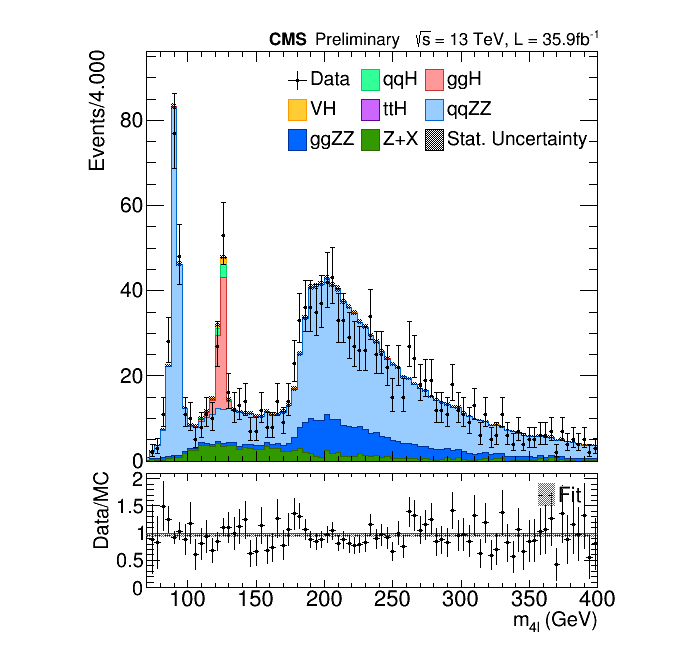
\includegraphics[scale=0.2,trim={2cm 1cm 2cm 1cm},clip]{figs/m4l_smhiggs_4l_full_range}\\
			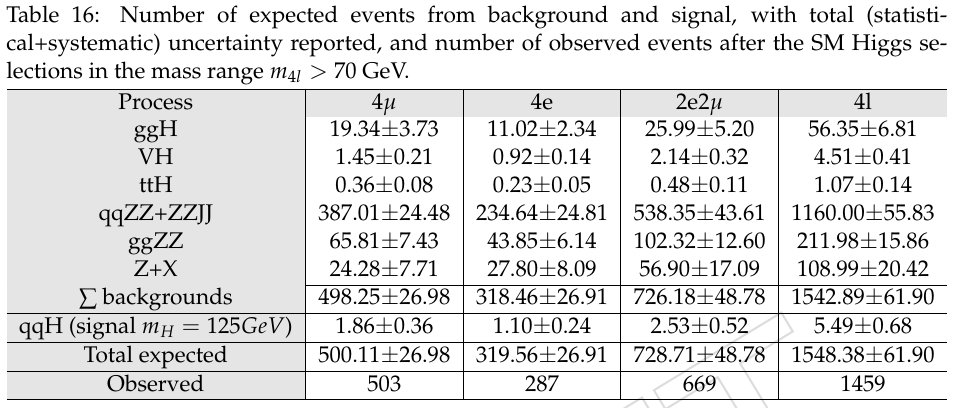
\includegraphics[scale=0.23]{figs/smhiggs_yields_table}
		\end{varblock}
		\begin{varblock}[5.8cm]{\centering After VBF-SR Selections}
			\centering
			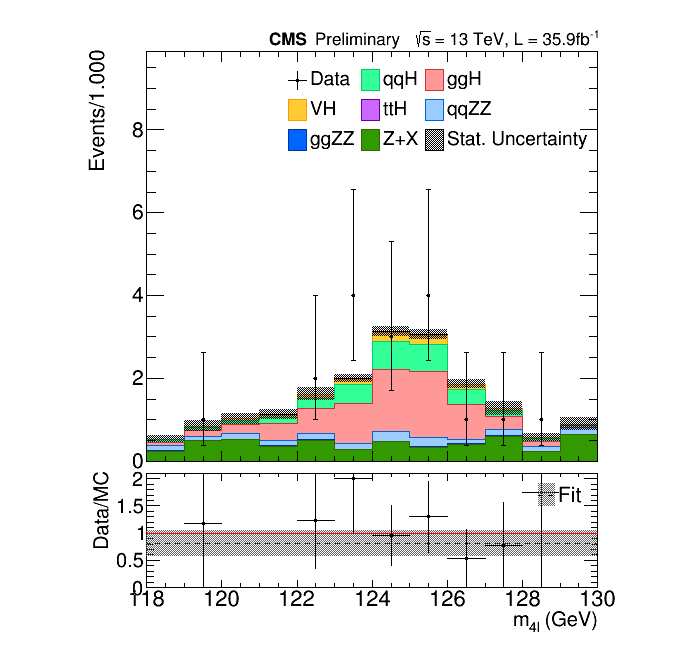
\includegraphics[scale=0.2,trim={2cm 1cm 2cm 1cm},clip]{figs/m4l_vbf_4l_118_130GeV}\\
			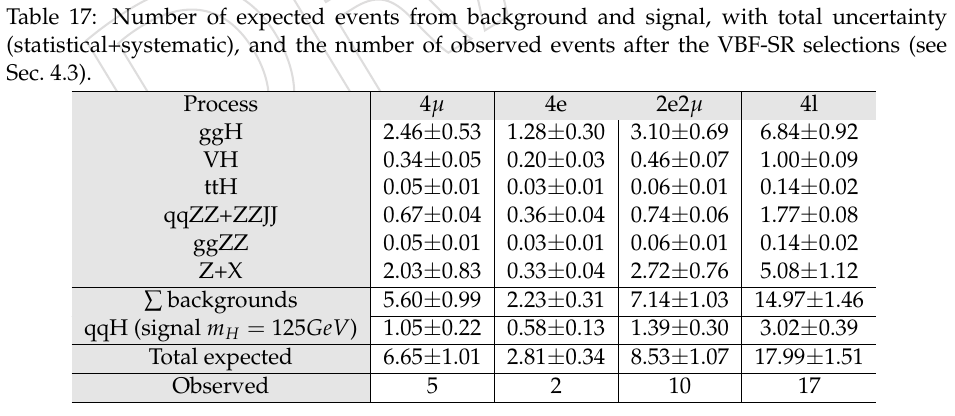
\includegraphics[scale=0.23]{figs/vbf_yields_table}
		\end{varblock}
	\end{multicols}	
\end{frame}

\subsection{Artificial Neural Networks (ANNs)}
\begin{frame}{Artificial Neural Networks (ANNs)}
	\begin{itemize}
		\justifying
		\item Functionals coming from Machine Learning field (closest field to development of Artificial Intelligence) in Computer Science;
		\item ANNs have been successfully applied in many tasks as recognition of hand-written digits, images, sounds, sequences of data, play games, etc;
		\item Google and Microsoft are investing on them: Deep Mind, Cloud Machine Learning Engine, Cortana, Azure Studio, etc;
		\item An ANN is basically a function which the arguments are functions: $\Omega(x) =  \Phi(f_{1}(x), f_{2}(x), ..., f_{n}(x))$;
		\item It was inspired by neuron-science: how the brain works;
	\end{itemize}
	\center		
	\begin{overpic}[scale=0.22]{figs/neuron}
		\put(60,49){\footnotesize \color{blue}ANN neuron}
	\end{overpic}
	\quad
	\quad
	\begin{overpic}[scale=0.24]{figs/DNN}
		\put(0,65){\footnotesize\color{blue}Assembly many neurons to build a net}
		\put(25,0){\footnotesize\color{red}Depth reduces width}
	\end{overpic}
\end{frame}	

\begin{frame}{Artificial Neural Networks (ANNs)}
	\vspace{-0.1cm}	
	\begin{itemize}
		\justifying
		\item Training an ANN consists in finding parameters ($w_{i}$ and $b_{i}$) for $\Omega(x)$, such that it models a dataset in the best (possible) way;
		\item Supervised ANN training:
		\vspace{-0.3cm}
		\begin{multicols}{2}
		\begin{itemize}
		\justifying
			\item Present examples to ANN and their expected $\Omega(x)$ outputs;
			\item Computes difference between expected and NN predictions;
			\item Update $w_{i}$ and $b_{i}$ using this difference;
			\item Repeat until predictions are good enough (minimize the difference);
		\end{itemize}
		\centering
		\begin{overpic}
			[width=3.5cm,height=1.5cm]{figs/ann_supervised_learning}
			\put(-10,30){\textbf{X}}
			\put(102,30){\scriptsize $\Omega($\textbf{X})$_{pred}$}
			\put(92,40){\scriptsize $\mathcal{E}(\Omega_{exp}-\Omega_{pred})$}
			\put(26,21){\tiny $\Delta w_{ji} (n) \propto \eta \frac{\partial \mathcal{E}}{\partial w_{ji}}$}
			\put(27,36){\scriptsize $w_{ji}(n)$, $b_{ji}(n)$}
			\put(19,3){\scriptsize $w_{ji}(n+1)$, $b_{ji}(n+1)$}
		\end{overpic}
		\end{multicols}
		\vspace{-0.3cm}
		\item Here's an ANN learning $f(x) = a.x + b$ (just a linear dataset):
	\end{itemize}
	\centering
	\movie[height=4.6cm,width=11.8cm,loop,showcontrols]{
		\begin{overpic}
			[height=4.6cm,width=11.7cm]{figs/tonystark_jarvis}
			\put(42,35){\color{red}\large{Wake up Jarvis!}}
		\end{overpic}
	}{figs/nn_learning_linear_data.mp4}\\
	\tiny \url{https://www.youtube.com/watch?v=XAF1skB_MUw}
\end{frame}	

%\begin{frame}{Artificial Neural Networks (ANNs)}
%	\begin{block}{\centering Briefly Overview}
%		\begin{center}
%			\begin{overpic}[scale=0.25]{figs/neuron}
%				\put(17,59){\footnotesize \color{blue}Neuron (node/activation)}
%			\end{overpic}
%			\begin{overpic}[scale=0.29]{figs/DNN}
%				\put(25,0){\footnotesize\color{red}Depth reduces width}
%			\end{overpic}
%		\end{center}
%		{\color{blue}Neuron}: NN basic unit that associates inputs to an output. A NN is a set of connected neurons.\\
%		{\color{blue}Training}: weights ($w_{i}$) and bias ($b$) in each neuron are adjusted to minimize NN model error on mapping inputs to outputs. \\
%		{\color{blue}Deep Learning}: training methods for deep NN.
%	\end{block}	
%\end{frame}	

\begin{frame}{MC Preparation for ANN Training}
	\begin{itemize}
		\justifying
		\item For the ANN studies the MCs\footnote{Data is not used on ANN training.} are prepared in the following way:
		\item The channels (4e, 4$\mu$ and 2e2$\mu$ selected separately) are merged into just a sample for each MC (the channels are randomized inside the sample);
		\item Each merged sample are split into 2 independent sets:
		\begin{itemize}
		\justifying 
			\item \textbf{Training}: contains 80$\%$ of all events (from each sample) and is used to train ANNs;
			\item \textbf{Testing}: contains remaining 20$\%$ of events and is used to test ANN after training;
		\end{itemize}
		\item Then each set of all MCs are merged (and randomized) to compose the final training/testing input set to train/test ANNs;
		\item Additionally, two subsets have been defined based on the available number of jets per event:
		\begin{itemize}
		\justifying
			\item \textbf{Njets2}: only events with exactly two jets;
			\item \textbf{Njets3}: only events with at least three jets;
		\end{itemize}
		\item ANNs are built and trained via the open-source {\color{red}Keras}\footnote{{\color{blue}\url{https://keras.io/}} (now interfaced with TMVA).} (standard ML community tool) python package;
	\end{itemize}		
\end{frame}

\begin{frame}{Training Strategy}
	\begin{itemize}
		\justifying
		\item It's hard to assure a set of parameters as the best one;
		\item ANN architecture optimization by scanning over several parameters;
		\item One ANN chosen for each Njets case via $max(\epsilon.\pi)$ (ie. efficiency $\times$ purity);
	\end{itemize}
	\begin{block}{\centering Training parameters (focus on low level variables)}
	\centering
	\begin{tabular}{c|l}
		\hline
		\textbf{Parameter}      & \textbf{Tested options}\\
		\hline
		Inputs         & leptons/jets($p_{T}$,$\eta$,$\phi$), MET\\
		\hline
		Pre-processing & none, normalization, standardization\\
		\hline
		Topologies\footnote{\tiny That refers to hidden layers. The output layer is always single sigmoid neuron}     & 7:5:3, 21:13:8, 10:10:10:10, 30, 100, ...\\
		\hline
		Early stop\footnote{\tiny Number of epochs to stop training if no improvement occurs.}     & 100, 600, 3000\\
		\hline
		Minimizer\footnote{\tiny Method used to compute parameters update.}      & SGD, Adam, Adagrad, Adadelta, RMSprop\\
		\hline
		Batch size\footnote{\tiny Subset from training set used to get parameters updates. N batches = N iterations per epoch.}     & 1, 5, 32, 64, 128, 786\\
		\hline
		Neuron         & ReLU, SeLU\\
		\hline
		Loss scaling\footnote{\tiny It's possible to use weights in training to optimize discrimination.}   & XS (process total XS), $\sigma.\epsilon.BR$ (event weight)\\
		\hline
		Dropout\footnote{\tiny Fraction of inputs randomly set to zero durging training.} & none, 0.1, 0.3, 0.5, 0.7, 0.9, 0.99, 0.3:0.4:0.2, 0.5:0.25:0.1\\
		\hline
	\end{tabular}		
	\end{block}
\end{frame}

\begin{frame}{ANNs Shape for Njets2, Njets3 and their Combination}
	\begin{itemize}
		\justifying
		\item Here are the (final) two ANNs chosen as VBF discriminants in each jet-based category and their combination;
	\end{itemize}
	\begin{multicols}{3}
		\begin{varblock}[3.8cm]{\centering Njets2}
			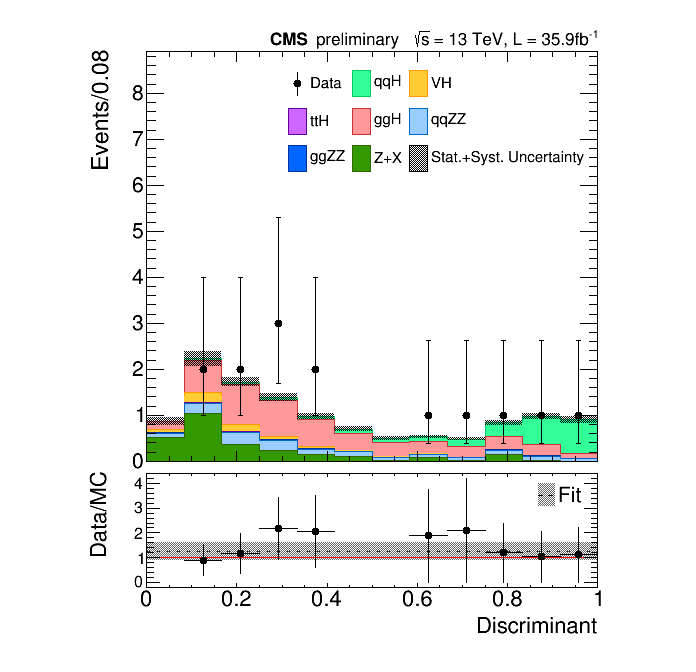
\includegraphics[scale=0.2,trim={3cm 1cm 3cm 1cm},clip]{figs/k57nj2_shapes_prefit}
		\end{varblock}
		\begin{varblock}[3.8cm]{\centering Njets3}
			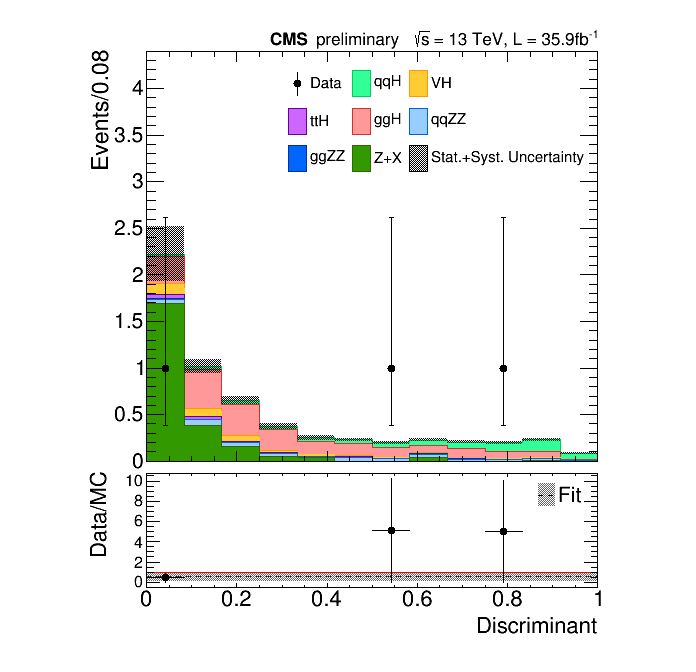
\includegraphics[scale=0.2,trim={3cm 1cm 3cm 1cm},clip]{figs/k24nj3_shapes_prefit}
		\end{varblock}		
		\begin{varblock}[3.8cm]{\centering Njets2+Njets3}
			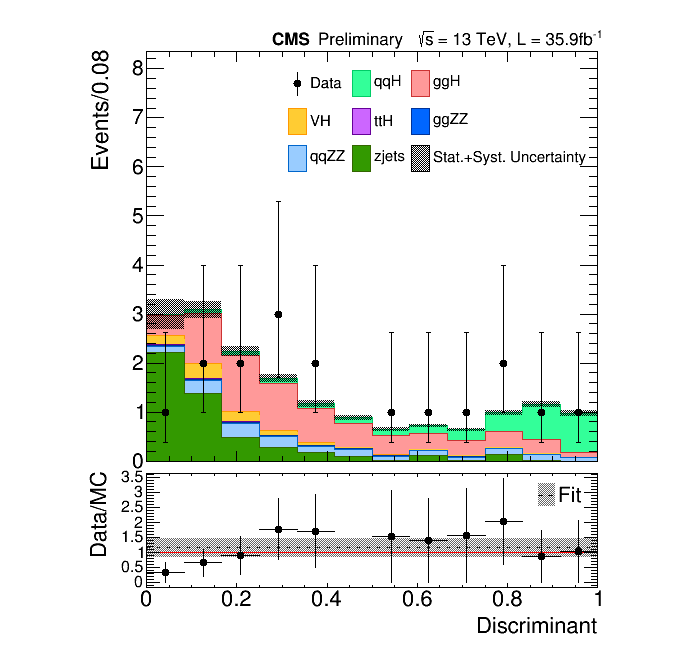
\includegraphics[scale=0.2,trim={3cm 1cm 3cm 1cm},clip]{figs/k57nj2_k24nj3_shapes_prefit}
		\end{varblock}				
	\end{multicols}
	\begin{itemize}
		\justifying
		\item $Z+X$ shape derived by feeding NNs with observed Data and $ZZ$ MC \footnote{Note that, the FR doesn't need to be redone.} and, repeating the procedure previously explained for this background estimation;
	\end{itemize}
\end{frame}

\subsection{Systematic Uncertainties}
\begin{frame}{Experimental and Theoretical Systematic Uncertainties}
	\begin{itemize}
		\justifying
		\item Experimental and Theoretical systematic uncertainties accounted in this analysis (enter as log-normal nuisance parameters in the statistical analysis):
	\end{itemize}	
	\begin{multicols}{2}
		\begin{varblock}[5.4cm]{\centering Experimental Uncertainties}
			\centering
			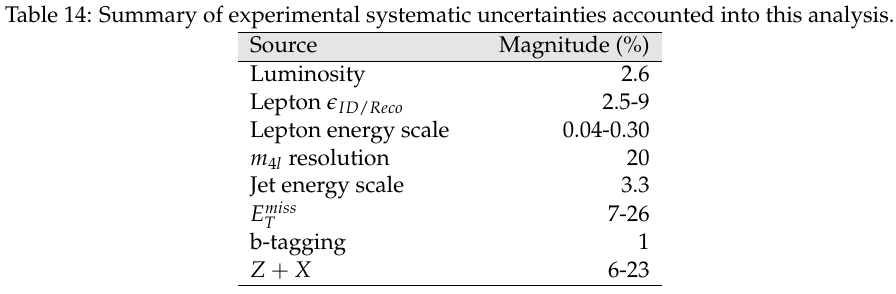
\includegraphics[scale=0.46,trim={6cm 0cm 6cm 0.8cm},clip]{figs/experimental_sys_uncs}
		\end{varblock}
		\begin{varblock}[5.9cm]{\centering Theoretical Uncertainties}
			\centering
			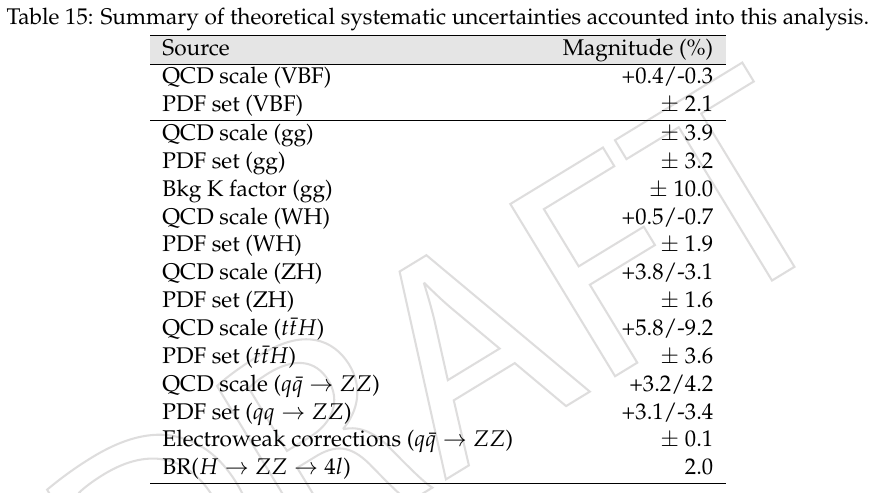
\includegraphics[scale=0.39,trim={4cm 0cm 4cm 0.8cm},clip]{figs/theoretical_sys_uncs}
		\end{varblock}
	\end{multicols}
	\begin{itemize}
		\justifying
		\item The systematic uncertainties on the VBF ANN discriminants are added into the statistical analysis via their nominal and shifted shapes;
	\end{itemize}
\end{frame}

\begin{frame}{ANN Discriminants Systematic Uncertainties}
	\begin{itemize}
		\justifying
		\item Systematic uncertainties on the ANN discriminants have been estimated from two sources: the systematic uncertainty on their inputs and the systematic uncertainty on the 3$^{rd}$ jet;
		\item The first case (which affect both jet-based categories) the systematic uncertainty on the ANN discriminants shape and yield has been derived by feeding the discriminants with the $\pm$1$\sigma$ shifted value of each input;
		\item The shifts are produced from one input variable at a time, such that, in the end there are $N_{(Inputs)} \times [1+2.N_{(InputsUncertainties)}]$ ANN distributions, including the nominal and shifted shapes;
		\item This procedure follows similar idea applied in previous CMS analysis:
		\begin{itemize}
		\justifying
			\item \url{cms.cern.ch/iCMS/jsp/openfile.jsp?tp=draft&files=AN2012_141_v9.pdf}
			\item \url{https://cds.cern.ch/record/2205282}
			\item \url{https://cds.cern.ch/record/2273847}
		\end{itemize}
	\end{itemize}
\end{frame}

\begin{frame}{ANN Discriminants Systematic Uncertainties}
	\begin{itemize}
		\justifying
		\item Here is an example of nominal and shifted distributions (superimposed) from one ANN for qqH and ggH (largest background) processes;
		\item The shifts look good and under control (in other words the discriminants are stable), mainly for the signal;
	\end{itemize}
	\center
	\vspace{-0.2cm}
	\begin{overpic}
		[scale=0.45,trim={7cm 0cm 0cm 0cm},clip]{/media/micah/DATA/cernbox/MonoHiggsHZZ4L/KerasV5/Uncertainty/datacard_root_example}
		\put(80,75){\color{red}\textbf{qqH}}
		\put(20,75){\color{blue}\textbf{ggH}}
	\end{overpic}
\end{frame}

\begin{frame}{ANN Discriminants Systematic Uncertainties}
	\begin{itemize}
		\justifying
		\item Since this analysis is proposing the usage of the 3$^{rd}$ jet and is not possible:
		\begin{itemize}
		\justifying
			\item to replace the current VBF MC sample (VBF-H2J) by its NLO VBF-H3J version\footnote{Process VBF\_HJJJ available at PowhegV2 (private generation following 2016 configurations).};
			\item or merge the two MC samples in suitable way;
		\end{itemize}
		\item A systematic uncertainty\footnote{It affects only Njets3 category.} because of using the 3$^{rd}$ jet from the current VBF MC sample has been estimated by computing the ratio between the ANN distribution using VBF-H2J and VBF-H3J, separately per four-lepton channel:
	\end{itemize}
	\begin{multicols}{3}
		\begin{varblock}[3.8cm]{\centering $4\mu$}
			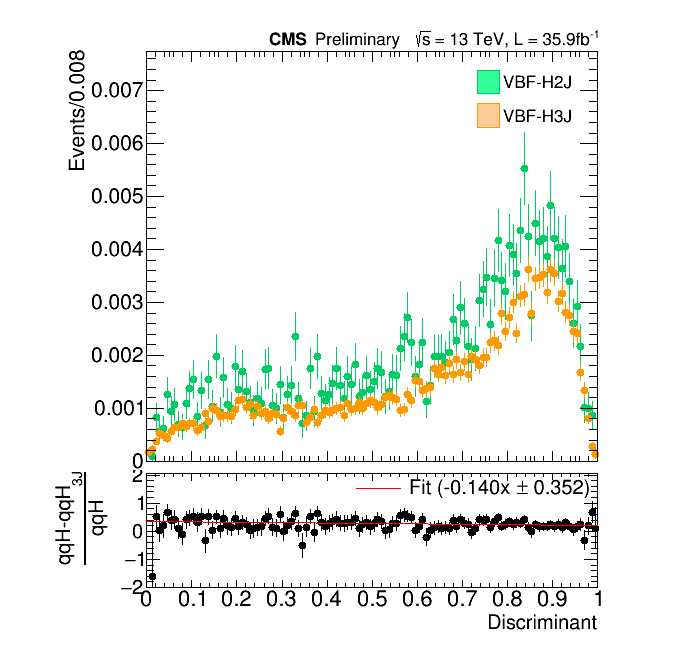
\includegraphics[scale=0.19,trim={1.5cm 1cm 3cm 1cm},clip]{figs/k24nj3_3rdJetUncertainty_4mu}
		\end{varblock}
		\begin{varblock}[3.8cm]{\centering $4e$}
			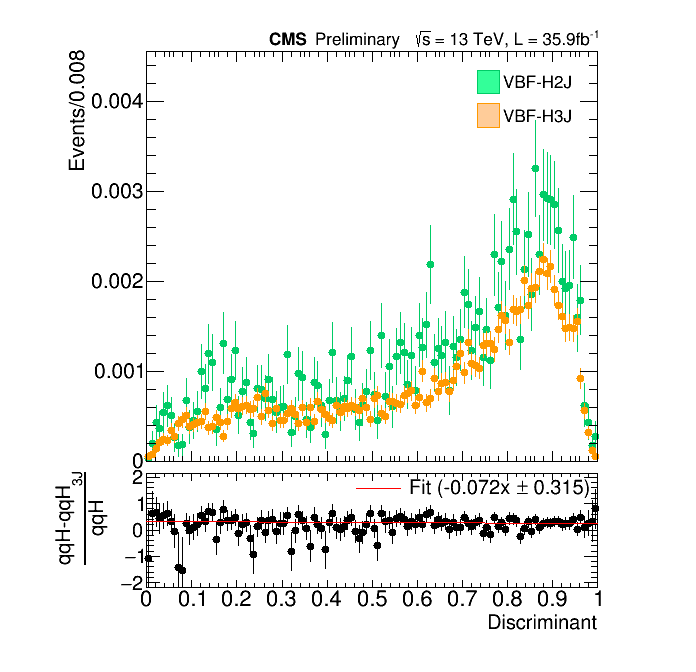
\includegraphics[scale=0.19,trim={1.5cm 1cm 3cm 1cm},clip]{figs/k24nj3_3rdJetUncertainty_4e}
		\end{varblock}		
		\begin{varblock}[3.8cm]{\centering $2e2\mu$}
			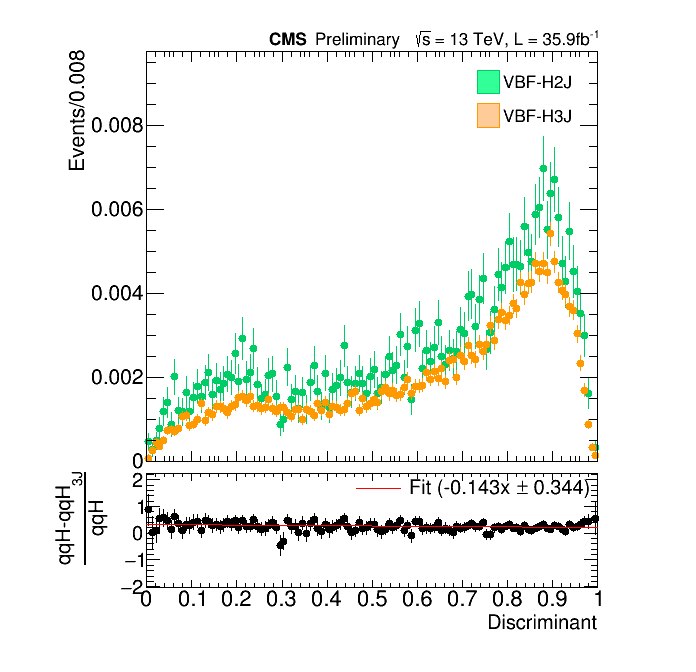
\includegraphics[scale=0.19,trim={1.5cm 1cm 3cm 1cm},clip]{figs/k24nj3_3rdJetUncertainty_2e2mu}
		\end{varblock}				
	\end{multicols}	
\end{frame}
		
\subsection{Statistical Analysis and Results}
\begin{frame}{Statistical Analysis}
	\begin{itemize}
		\justifying
		\item The statistical analysis is carried through Higgs Combine tool;
		\item A 1D binned shape analysis is performed on the VBF ANN discriminants, separately for each jet-based category and for their combination (using Combine tool);
		\item Inputs are the ANN discriminants via 1D histograms, containing the proper signal and background normalizations, along with the statistical and systematical uncertainties;
		\item Due to the low statistics of this analysis the HybridNew (fully Frequentist) method has been used (50k toys);
		\item Results achieved by combining the ANN discriminants from each jet-based category are highlighted in the next slides;
	\end{itemize}
\end{frame}

\begin{frame}{Statistical Analysis}
	\begin{itemize}
		\justifying
		\item The VBF signal strength is measured to be $\mu \equiv \sigma^{Obs}_{qqH} / \sigma^{SM}_{qqH} = 1.28_{-0.84}^{+1.24}$ by combining ANN discriminants of Njets2 and Njets3 categories;
	\end{itemize}
	\vspace{-0.5cm}
	\begin{figure}
		\centering
		\subfloat[$\mu_{qqH}$ likelihood scans.]{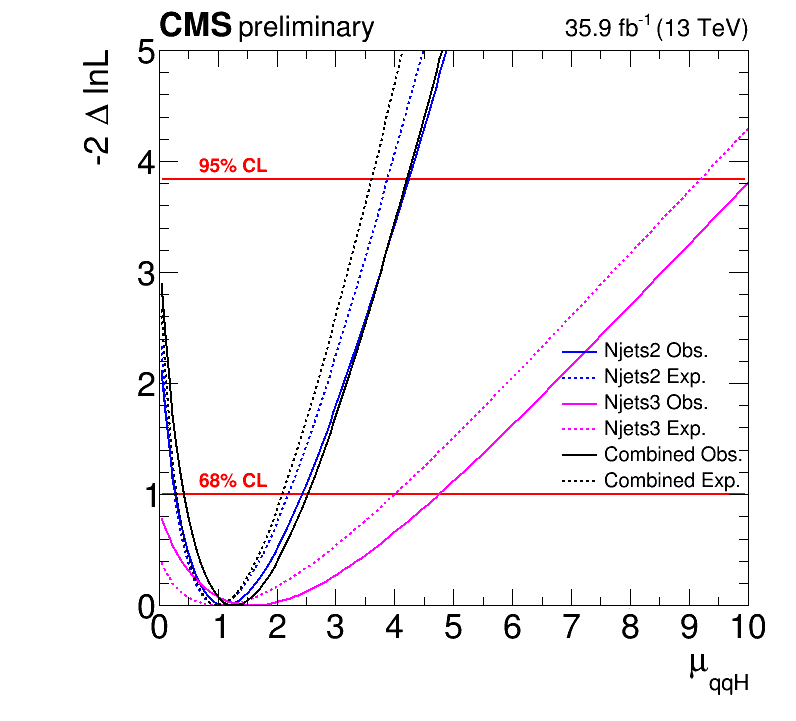
\includegraphics[scale=0.2]{figs/LikelihoodScans}}
		\subfloat[$\mu_{qqH}$ best fit on each channel.]{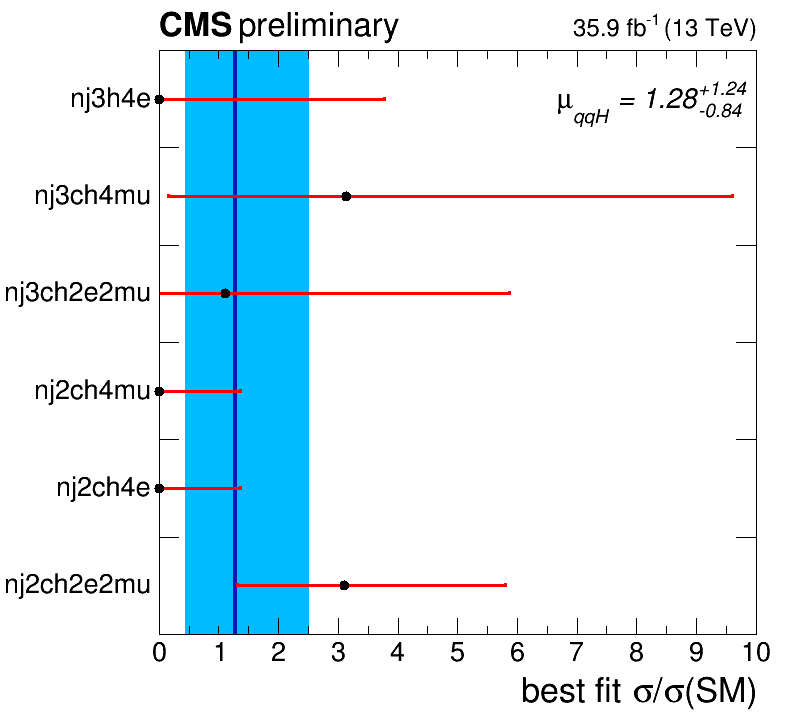
\includegraphics[scale=0.2]{figs/ChannelsCompatibility}}
	\end{figure}
	\vspace{-0.5cm}
\begin{table}
	\caption{Expected and observed signal strength modifiers from each category and four-lepton channel for 35.9fb$^{-1}$ of observed data at $\sqrt{s}=$ 13TeV.}
	\centering
	\footnotesize
	\begin{tabular}{c|c|c|c|c|c|c|c}
		\hline
		Signal strength & $\mu_{qqH}^{4\mu,2J}$ & $\mu_{qqH}^{4e,2J}$ & $\mu_{qqH}^{2e2\mu,2J}$ & $\mu_{qqH}^{4\mu,3J}$ & $\mu_{qqH}^{4e,3J}$ & $\mu_{qqH}^{2e2\mu,3J}$ & $\mu_{qqH}^{4l,2J+3J}$\\
		\hline
		Expected & 1.00$^{+2.13}_{-1.49}$ & 1.00$^{+3.11}_{-1.00}$ & 1.00$^{+1.83}_{-0.96}$ & 1.00$^{+5.79}_{-1.00}$ & 1.00$^{+8.24}_{-1.00}$ & 1.00$^{+4.67}_{-1.00}$ & 1.00$^{+1.08}_{-0.70}$ \\
		\hline
		Observed & 0.00$^{+1.36}_{-0.00}$ & 0.00$^{+1.36}_{-0.00}$ & 3.10$^{+2.69}_{-1.79}$ & 3.13$^{+6.47}_{-2.98}$ & 0.00$^{+3.78}_{-0.00}$ & 1.10$^{+4.77}_{-1.14}$ & 1.28$^{+1.24}_{-0.84}$ \\ 
		\hline
	\end{tabular}
\end{table}	
\end{frame}

\begin{frame}{Statistical Analysis}
	\begin{itemize}
		\justifying
		\item Limits and significances have been computed via the HybridNew method:
		\begin{itemize}
		\justifying
			\item Limits show that hypothesis of VBF events in the present analysis can't be excluded, setting $\mu_{qqH}^{Obs} < 3.8$ and $\mu_{qqH}^{Exp} < 1.7$ at 95$\%$CL;
			\item Significances obtained are $\sigma_{qqH}^{Obs} = 1.9$ and $\sigma_{qqH}^{Exp} = 1.8$;
		\end{itemize}
	\end{itemize}
	\begin{figure}
		\centering
		\subfloat[Upper limits on $\mu_{qqH}$.]{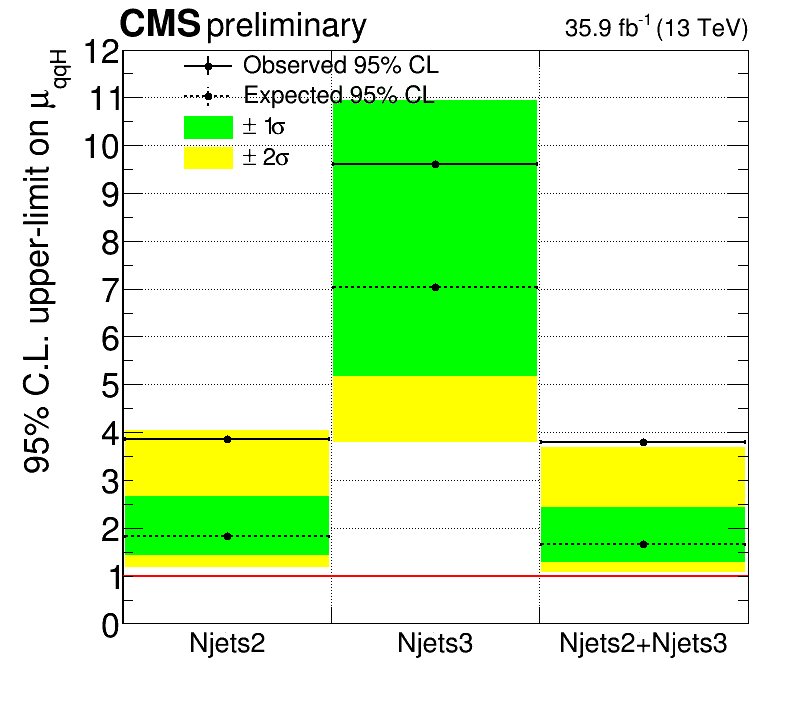
\includegraphics[scale=0.2]{figs/Limits}}
		\subfloat[Significances via the present analysis.]{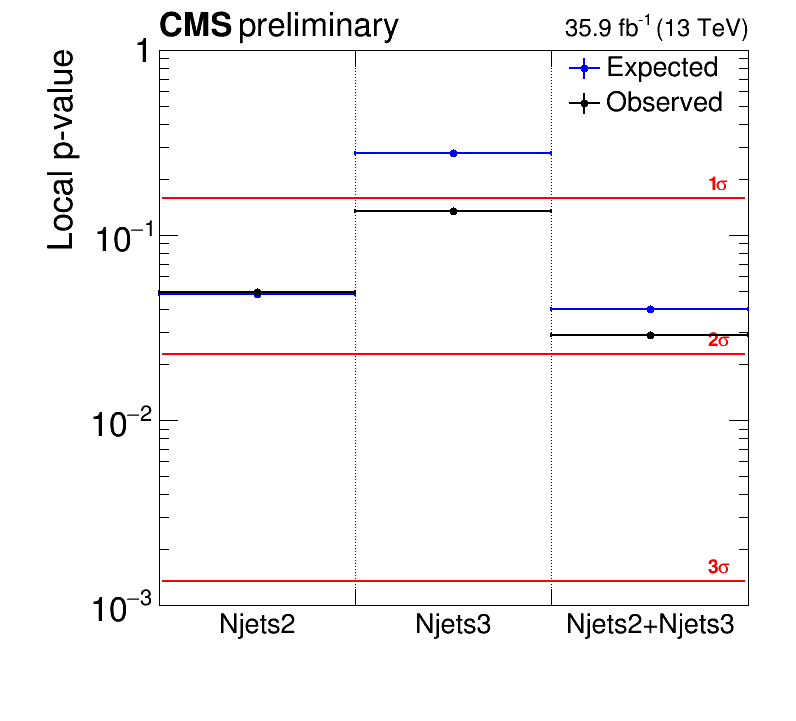
\includegraphics[scale=0.2]{figs/Pvalues}}
	\end{figure}
\end{frame}

\begin{frame}{Projections for Future Luminosities}
	\begin{multicols}{2}
	\begin{minipage}{6cm}
	\begin{itemize}
		\justifying
		\item The VBF signal strength measurement and the significance of the present analysis has been projected for future luminosities scenarios at the LHC;
		\item Systematic uncertainties have been accounted by scaling the present luminosity;
		\item The total uncertainty on the measurement of $\mu_{qqH}$ is expected to reduce $\sim$87$\%$ at $L = 150$fb$^{-1}$;
		\end{itemize}
	\end{minipage}
	\begin{overpic}
	   [scale=0.2]{figs/ChannelsCompatibility_39fb_vs_150fb}
	   \put(35,90){35.9fb$^{-1}$ vs. 150fb$^{-1}$}
	\end{overpic}
	\end{multicols}
	\vspace{-0.5cm}
	\begin{itemize}
		\justifying
		\item Significance of 5.1$\sigma$ is expected for a luminosity 10x larger than the present one. Below is a scan of the expected VBF significance between the present luminosity (35.9fb$^{-1}$) and future scenarios at the LHC.
	\end{itemize}
	\vspace{-0.4cm}
	\begin{table}
	\centering
	\begin{tabular}{c|c|c|c|c|c|c|c}
		\hline
		Luminosity (fb$^{-1}$)       & 35.9 & 150.0 & 300.0 & 359.0 & 1077.0 & 1795.0 & 3000.0\\
		\hline
		Factor (x $L^{35.9fb^{-1}}$) & 1.00 & 4.18  & 8.36  & 10.00 & 30.00  & 50.00  & 83.57\\
		\hline
		Expected significance        & 1.8  & 3.4   & 4.7   & 5.1   & 8.6    & 10.9   & 14.0\\
		\hline
		\end{tabular}
	\end{table}	
\end{frame}

\begin{frame}{Most $\&$ Least VBF-Like Event Display in each Category}
\centering
\vspace{0.6cm}
\begin{overpic}
	[scale=0.22]{figs/event_display_Run278167_Lumi1564_Event2852832207_Njets2_ANN0p93_DoubleEG_Run2016F_2}
	\put(30,63){ANN score: 0.93}
	\put(80,65){Njets2 Category}
\end{overpic}
\begin{overpic}
	[scale=0.22]{figs/event_display_Run275658_Lumi216_Event425010503_Njets2_ANN0p15_DoubleEG_Run2016C_2}
	\put(30,63){ANN score: 0.15}
\end{overpic}\\[0.6cm]
\begin{overpic}
	[scale=0.22]{figs/event_display_Run278018_Lumi453_Event844012107_Njets3_ANN0p77_DoubleMuon_Run2016F_2}
	\put(30,63){ANN score: 0.77}
	\put(80,65){Njets3 Category}	
\end{overpic}
\begin{overpic}
	[scale=0.22]{figs/event_display_Run278018_Lumi361_Event673988874_Njets3_ANN0p04_DoubleEG_Run2016F_2}
	\put(30,63){ANN score: 0.04}
\end{overpic}
\end{frame}

\section{CMS L1 Tracking Trigger AM+FPGA}
\begin{frame}
	\center
	\begin{minipage}{10cm}
		\begin{varblock}[8cm]{}
			\center
			\huge \color{red} CMS Level 1 Tracking Trigger\\ Associative Memory + FPGA
		\end{varblock}
	\end{minipage}
\end{frame}

\subsection{Introduction}
\begin{frame}{Introduction}
	\begin{itemize}
		\justifying
		\item During his PhD the  author was involved into the CMS Level 1 Tracking Trigger AM+FPGA project:
		\begin{itemize}
		\justifying
			\item one of the three CMS-L1TT projects (CMS upgrade phase II - HLLHC):
			\begin{itemize}
		\justifying
				\item Inclusion of inner-tracker data as part of L1 trigger;
				\item Original tracker designed for $L_{inst.} \sim 10^{34}$ cm$^{-2}$.s$^{-1}$ and PU$_{Ave.} \sim$ 20-30;
				\item Expected in phase II: $L_{inst.} \sim 10^{34}$ cm$^{-2}$.s$^{-1}$ and PU$_{Ave.} \sim$ 140-200;
				\item Required decision time: 5$\mu$s;
				\item 500-1k Tb/s of data to be processed;
			\end{itemize}
			\item leaded by Fermilab working group;
			\item the project aims for the usage of Associative Memories in combination with FPGAs;
			\item the author studied and implemented new components on the available software:
			\begin{itemize}
		\justifying
				\item synthetic match;
				\item duplicate removal; 
				\item stub bending;
				\item road and combination truncation
				\item track fitter $\chi^{2}$ adjustment;
			\end{itemize}
			\item results have been produced with different high-lumi scenarios (2-10k events):
			\begin{itemize}
		\justifying
				\item ($\mu$/$\pi$/$e$)+PU(140,200,300,400);
				\item $\nu$+PU(140,200,250)  (simulates pure PU, low $p_{T}$ particles);
				\item $t\bar{t}$+PU200;
				\item jets($p_{T}=250GeV$)+PU200;
			\end{itemize}
			\item hardware work: board inspections and tests;
		\end{itemize}
	\end{itemize}
\end{frame}

\begin{frame}{The CMS-L1TT AM+FPGA Approach}
\begin{flushright}
	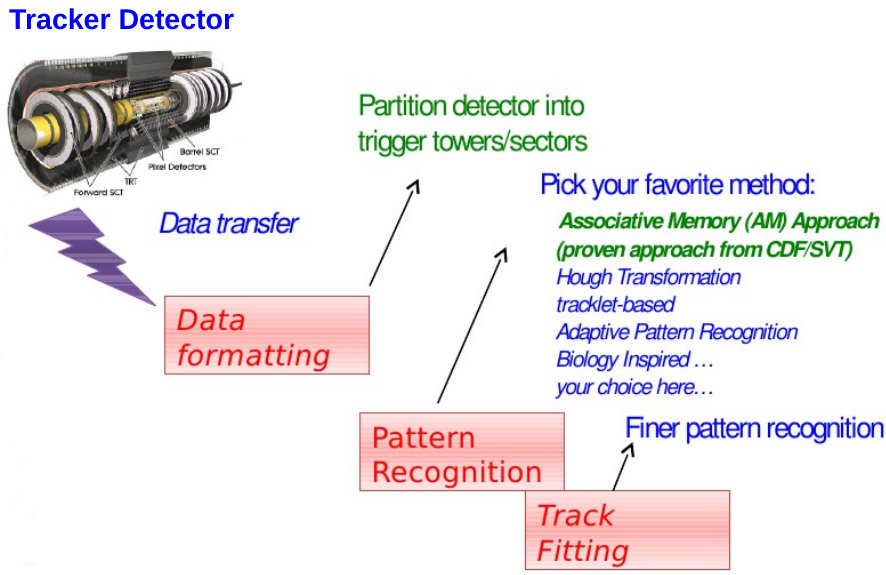
\includegraphics[scale=0.45]{CMSL1TTfigs/cms_l1TT_strategy}
\end{flushright}
\vspace{-1.8cm}
\begin{itemize}
	\begin{minipage}{5cm}
		\item The three CMS-L1TT projects can be divided into three stages:
	\end{minipage}
	\begin{itemize}
		\vspace{0.2cm}
		\begin{minipage}{6cm}
			\item \textbf{Data Formatting}: fragmentation of the CMS detector in $\eta-\phi$ sectors (trigger towers);
		\end{minipage}
		\begin{minipage}{10cm}
			\item \textbf{Pattern Recognition}: selection of coarse hits patterns (potentially real tracks);
		\end{minipage}
		\begin{minipage}{11cm}
			\item \textbf{Track Fitting}: extraction of refined track info using all hits from selected patterns;
		\end{minipage}
	\end{itemize}
\end{itemize}
\end{frame}

\begin{frame}{The CMS-L1TT AM+FPGA Approach}
	\begin{itemize}
		\justifying
		\item Here's the main idea and definitions adopted in the CMS L1TT AM+FPGA approach:
		\begin{itemize}
		\justifying
			\item \textbf{Superstrip (SS)}: cluster of hits in the detector layers. They receive an ID based on their $z-\phi$ position;
			\item \textbf{Road}: pattern of built from SS's;
		\end{itemize}
	\end{itemize}
	\begin{multicols}{2}
	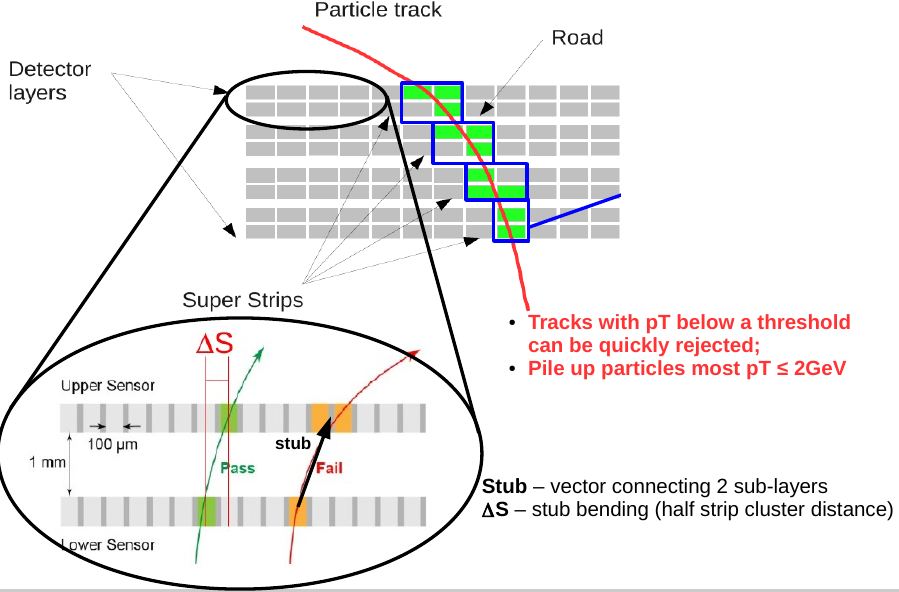
\includegraphics[scale=0.4,trim={0cm 0.1cm 0cm 0cm},clip]{CMSL1TTfigs/AMFPGA_scheme2}		
		\begin{itemize}
		\justifying
			\item An AM chip containing a big set of roads simulated via MC triggers the roads observed in real data. The hits from detector layers are processed in parallel;
			\item Once real roads are triggered, a set of possible hits combinations are built (possible tracks);
			\vspace{0.8cm}
			\item A fit select which combination is a real tracker;
		\end{itemize}
	\end{multicols}
\end{frame}

\subsection{Hardware Work}
\begin{frame}{The Hardware for the CMS-L1TT AM+FPGA}
\vspace{-2cm}
\begin{overpic}
	[scale=0.4]{CMSL1TTfigs/AMFPGA_scheme}
	\put(0,-30){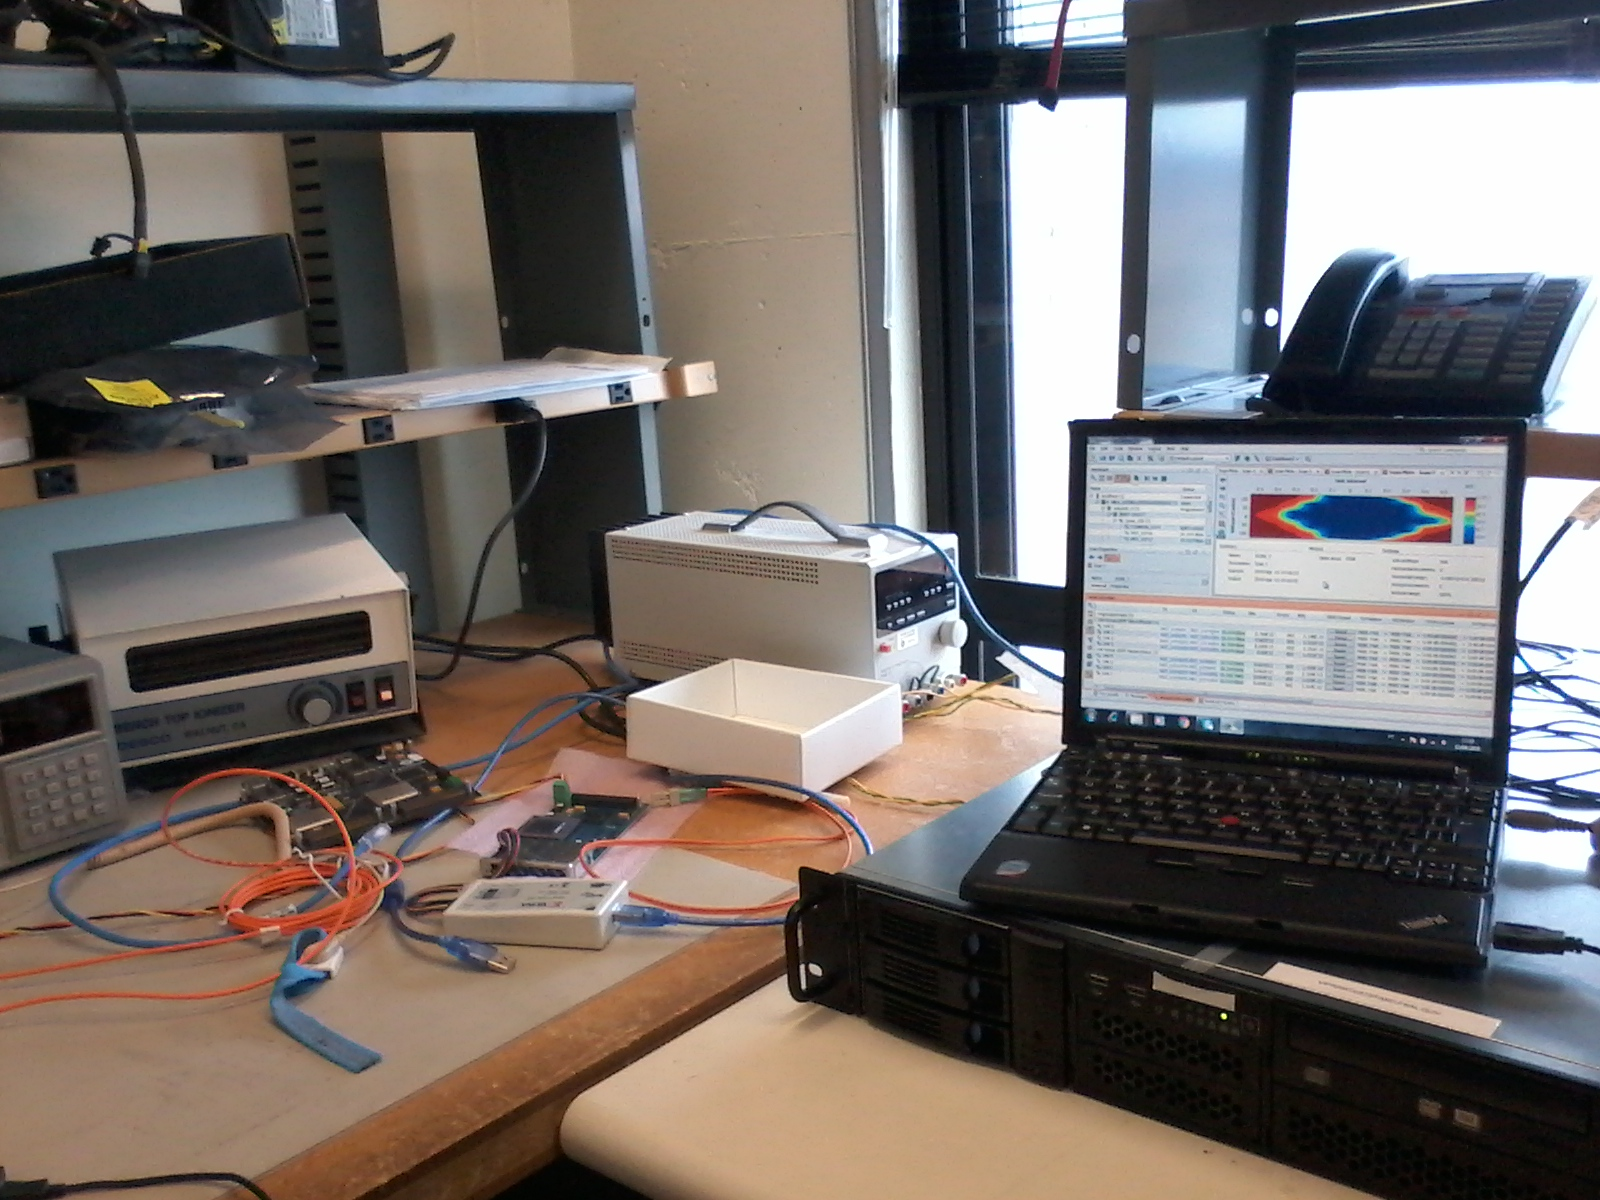
\includegraphics[scale=0.06]{CMSL1TTfigs/20160413_152420}}
	\put(36,-30){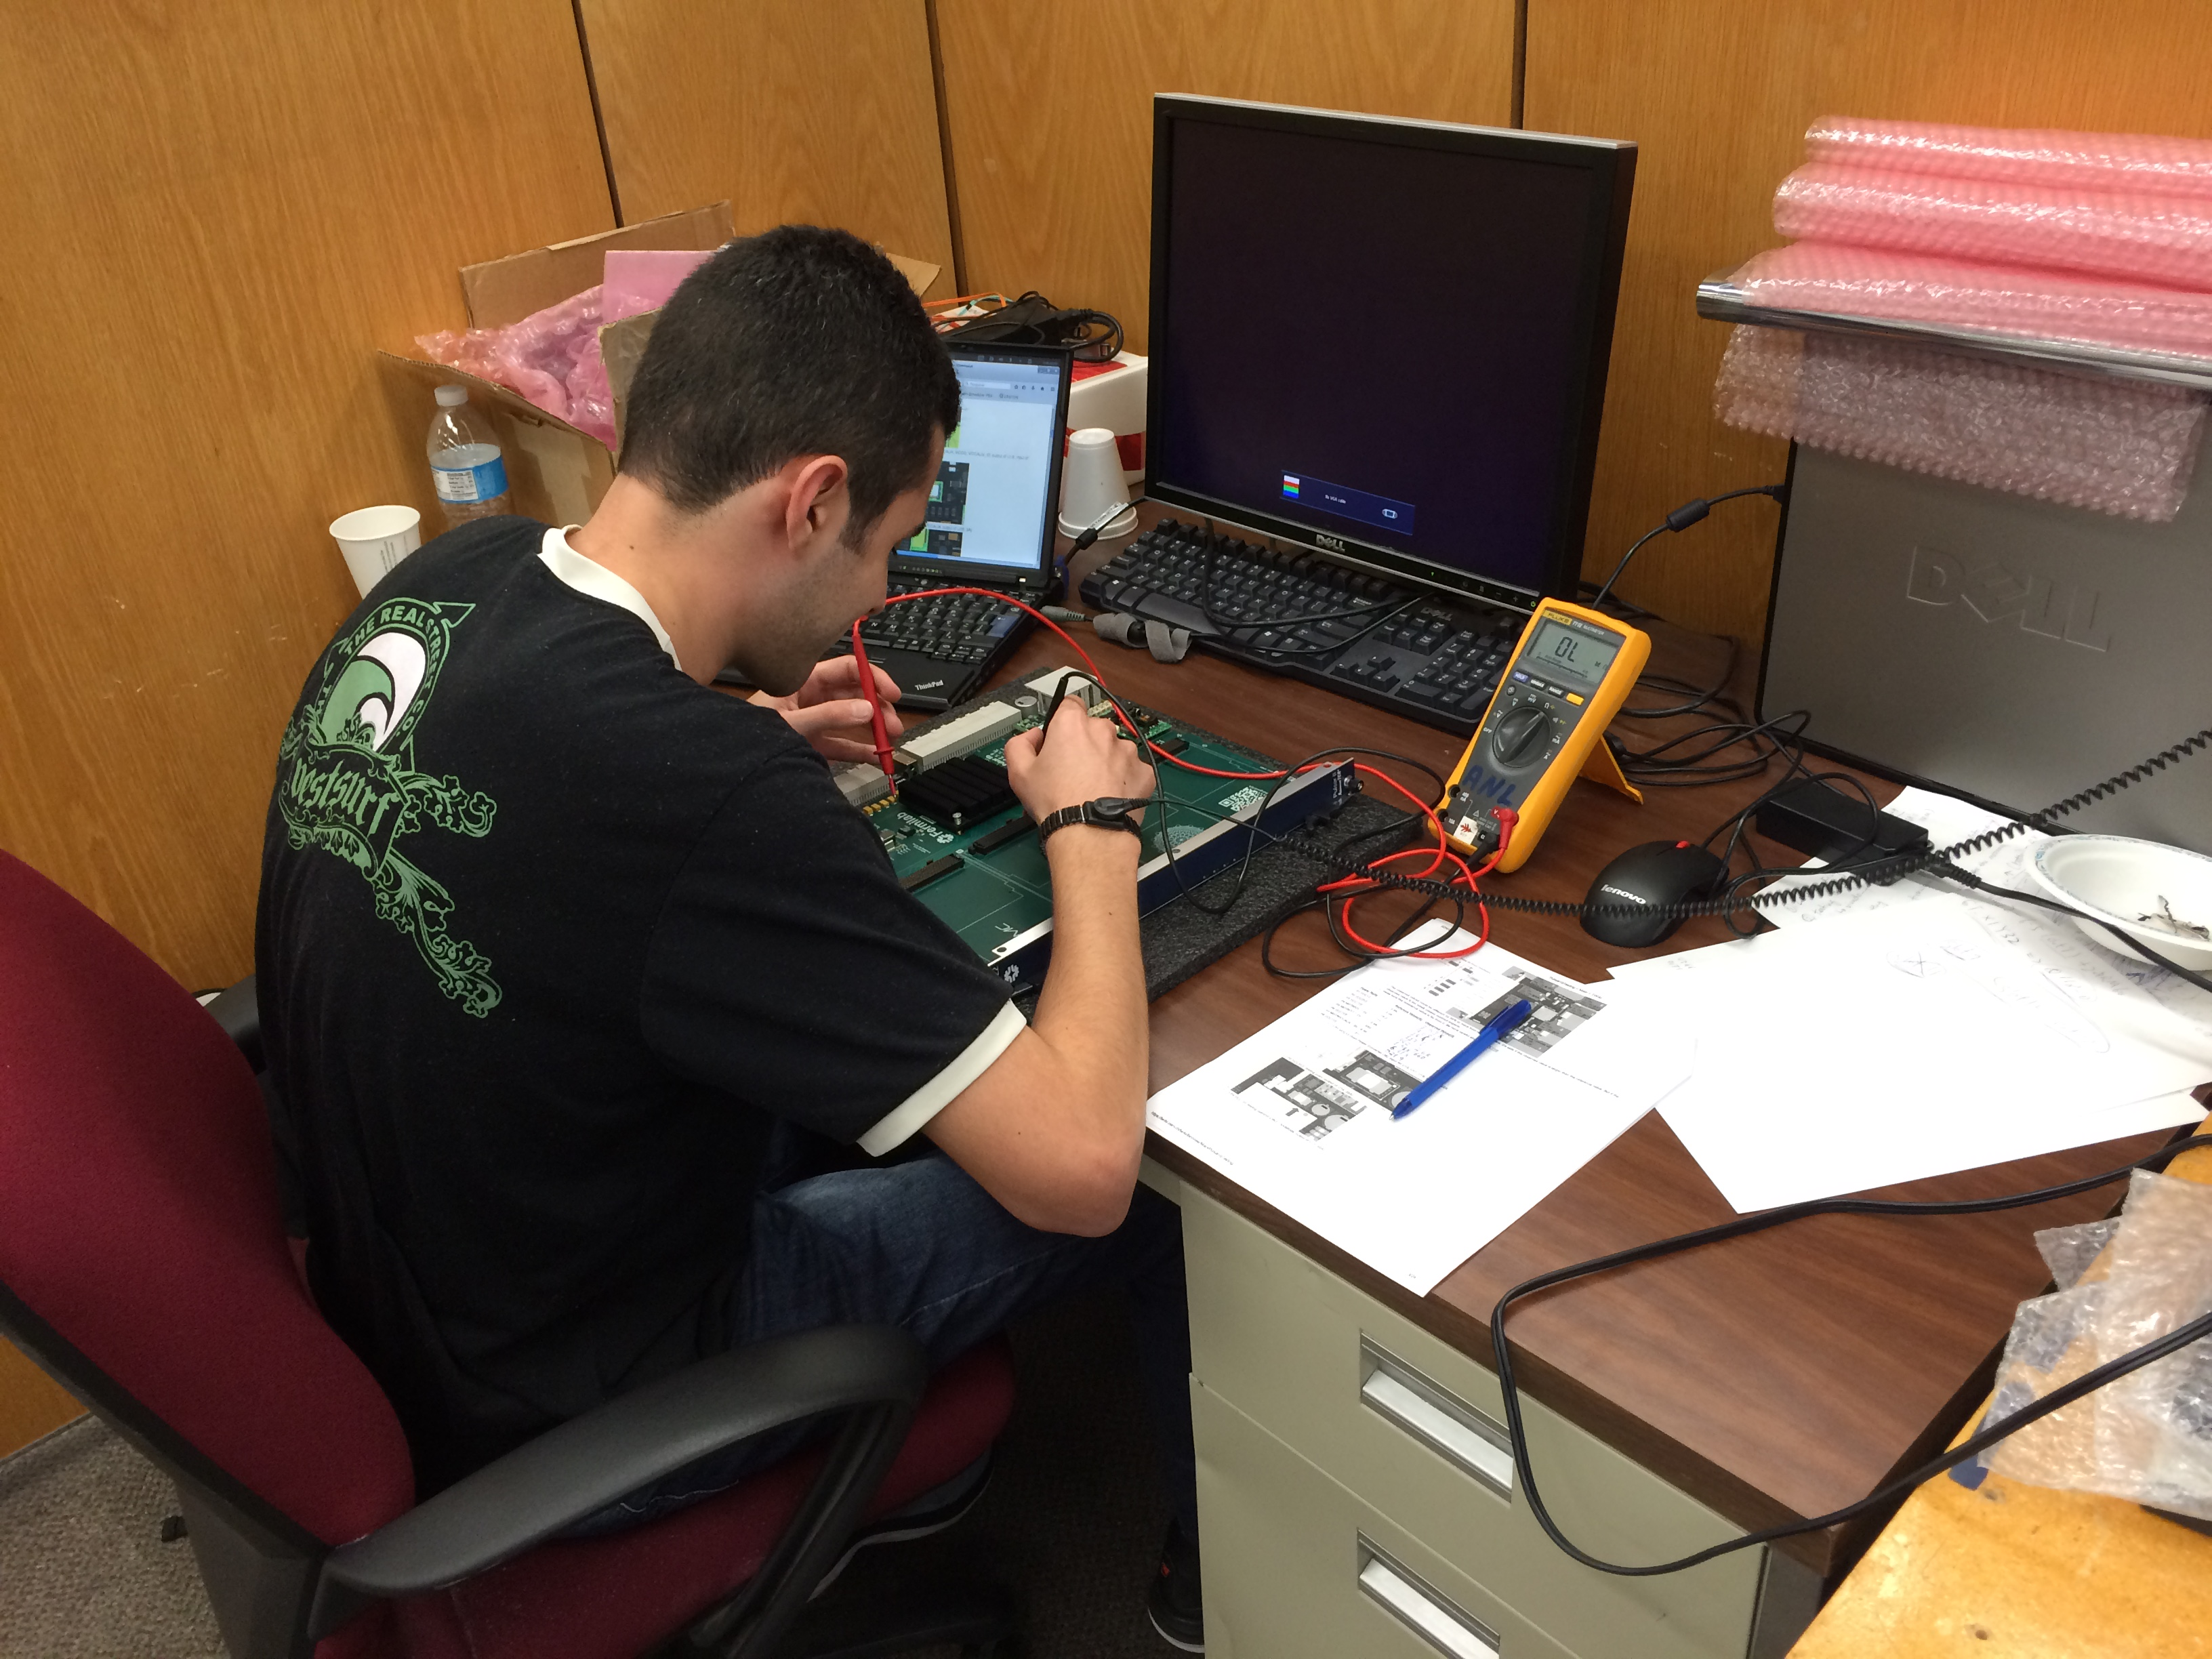
\includegraphics[scale=0.035]{CMSL1TTfigs/Foto-24-05-16-19-51-58}}
	\put(80,-23){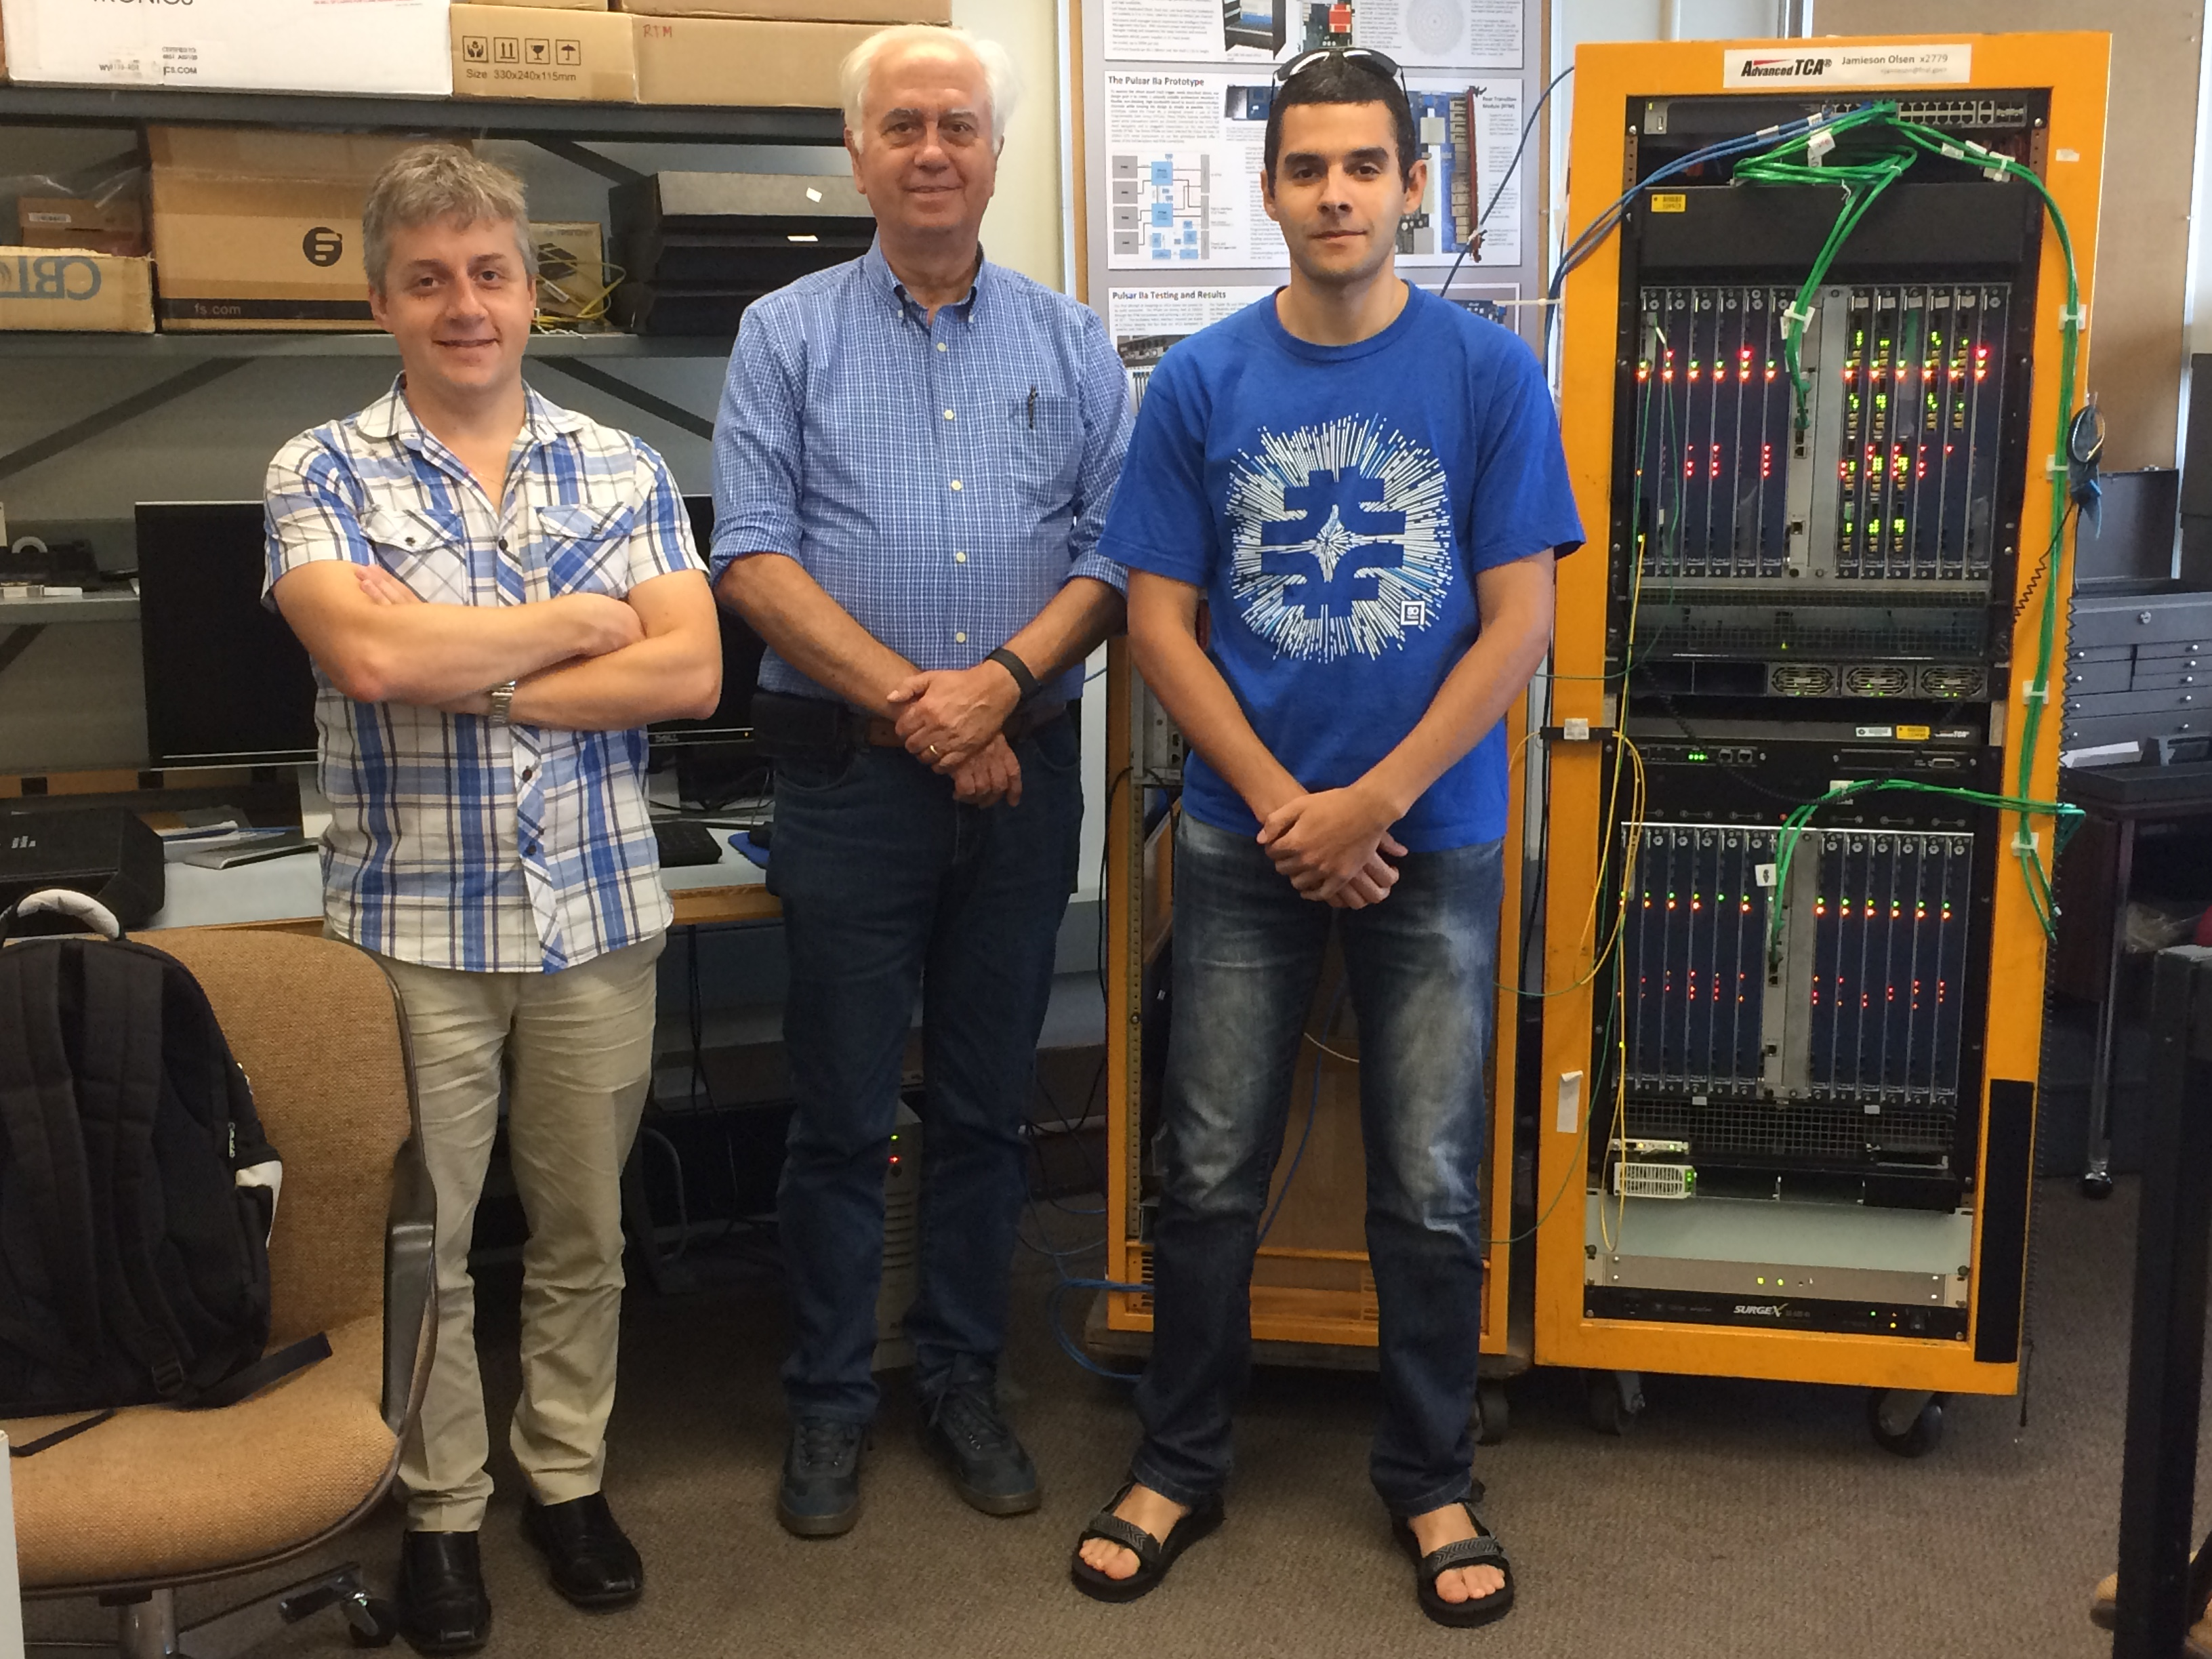
\includegraphics[scale=0.04]{CMSL1TTfigs/CMSL1TTAMFPGA_setup}}
\end{overpic}
\end{frame}

\subsection{Simulation Studies}
\begin{frame}{Simulation Studies: Roads and Combinations Truncation}
	\begin{multicols}{2}
	\begin{itemize}
		\justifying
		\item It was needed to check the approach under truncation of roads and combinations (for reducing latency, for instace);
		\item Implemented two new flags into the software for controlling the number of roads and combinations to be accepted for further processing;
		\item A study done by the author showed the smallest impact on the efficiency due to truncation happens when roads are sorted by frequency:
	\end{itemize}
	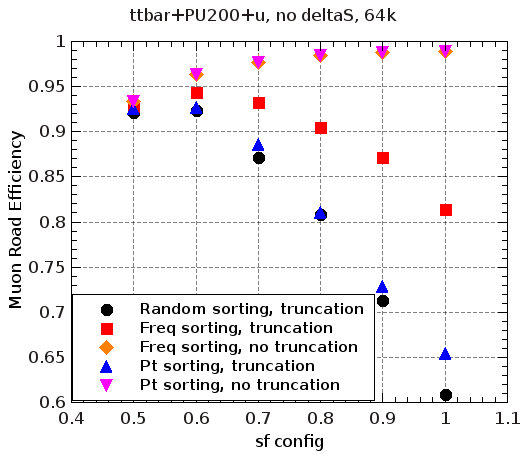
\includegraphics[scale=0.4]{CMSL1TTfigs/ttbar_pu200_mu_road_sorting_comparison}
	\end{multicols}
\end{frame}

\begin{frame}{Simulation Studies: Stub Bending ($\Delta S$)}
	\begin{multicols}{2}
	\begin{itemize}
		\justifying
		\item The stub bending is the core idea behind the CMS L1TT project:
		\begin{itemize}
		\justifying
			\item It helps to mitigate PU (mainly low $p_{T}$ particles);
		\end{itemize}
		\item In the AM+FPGA approach the $\Delta S$ prevents random patterns to be fired:
		\begin{itemize}
		\justifying
			\item Without $\Delta S$ an AM pattern can be triggered by hits coming from different real tracks crossing the detector layers in different angles:
		\end{itemize}
		\item The $\Delta S$ was encoded in the AM framework via the SS ID's. The following formula defines the SS ID when the stub bending is required:\\
		\begin{equation}
			\nonumber
			ss = i_{\Delta S} * N_{\phi} + i_{\phi}
		\end{equation}
	\end{itemize}
	\centering
	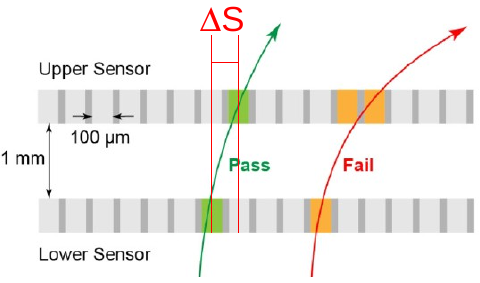
\includegraphics[scale=0.4]{CMSL1TTfigs/stub_definition}\\[0.2cm]
	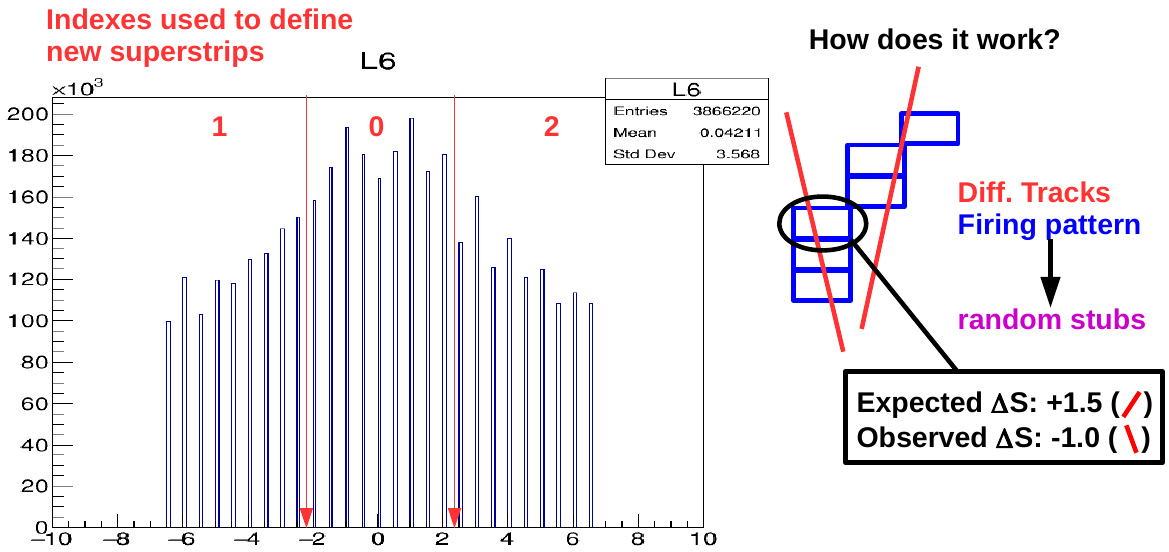
\includegraphics[scale=0.35,trim={20.5cm 2cm 0cm 2cm},clip]{CMSL1TTfigs/deltaS_approach}	
	\end{multicols}	
\end{frame}

\begin{frame}{Simulation Studies: Stub Bending ($\Delta S$)}
	\begin{itemize}
		\justifying
		\item The SS-$\Delta S$ formula:\\[-0.5cm]
	\begin{equation}
		\nonumber
		ss = i_{\Delta S} * N_{\phi} + i_{\phi}
	\end{equation}
	\begin{itemize}
		\justifying
		\item $i_{\Delta S}$: $\Delta S$ value of a given stub (max );
		\item $N_{\phi}$: number of trigger-tower segmentations in $\phi$;
		\item $i_{\phi}$: index of the $\phi$ segment which the stub belongs;
	\end{itemize}
	\item Two possibilities of building the SS ID's according to the $\Delta S$ values:
	\end{itemize}
	\vspace{0.2cm}
	\begin{multicols}{2}
		\centering
		\begin{overpic}
			[scale=0.3,trim={0cm 0cm 9cm 0cm},clip]{CMSL1TTfigs/ttbar_pu200_sym115577}
			\put(10,102){\textbf{Symmetric} (eg. SYM115577)}
		\end{overpic}
		\begin{overpic}
			[scale=0.3,trim={0cm 0cm 9cm 0cm},clip]{CMSL1TTfigs/ttbar_pu200_asym115577}
			\put(10,102){\textbf{Asymmetric}  (eg. ASYM115577)}
		\end{overpic}
	\end{multicols}	
\end{frame}

\begin{frame}{Simulation Studies: Stub Bending ($\Delta S$)}
	\begin{itemize}
		\justifying
		\item This $\Delta S$ approach allows the following schemes (negative ranges omitted):\\
	\begin{tabular}{c|c|l}
		\hline
		\hline
		$\#$ranges & range width & $\Delta S$ values ({\color{red}[~]} central ranges)\\
		\hline
		3 & 9 & {\color{red}[}-2.0, 2.0{\color{red}]}, [2.5, ...]\\
		5 & 7 & {\color{red}[}-1.5, 1.5{\color{red}]}, [2.0, 5.5], [6.0, ...]\\
		7 & 5 & {\color{red}[}-1.0, 1.0{\color{red}]}, [1.5, 3.5], [4.0, 6.0], [6.5, ...]\\
		9 & 3 & {\color{red}[}-0.5, 0.5{\color{red}]}, [1.0, 2.0], [2.5, 3.5], [4.0, 5.0], [5.5, ...]\\
		\hline 
	\end{tabular}
	\item Effect of $\Delta S$ on the number of roads and combinations:
	\begin{itemize}
		\justifying
		\item Reduction of up to $\sim$10x on roads and $\sim$50x on combinations;
		\item Symmetric method produces few more combs/roads than Asymmetric one;
	\end{itemize}
	\end{itemize}
	\centering
	\begin{overpic}
		[scale=0.3,trim={0cm 0cm 0cm 1cm},clip]{CMSL1TTfigs/ttbar_pu200_smu_roads_combs_deltaS}
		\put(15,6){$\mu @ t\bar{t}+PU200$}
	\end{overpic}
	\quad
	\begin{overpic}
		[scale=0.3,trim={0cm 0cm 0cm 1cm},clip]{CMSL1TTfigs/jet_Pt250_pu200_roads_combs_deltaS}
		\put(15,6){$jets(250GeV)+PU200$}
	\end{overpic}
\end{frame}

\begin{frame}{Simulation Studies: Stub Bending ($\Delta S$)}
	\begin{itemize}
		\justifying
		\item Effect of $\Delta S$ on the road efficiency:
		\begin{itemize}
		\justifying
			\item Up to 20$\%$ and 50$\%$ of efficiency can be recovered when truncation is applied;
		\end{itemize}
	\end{itemize}
	\centering
	\begin{overpic}
		[scale=0.4,trim={0cm 0cm 0cm 1cm},clip]{CMSL1TTfigs/ttbar_pu200_pt_split_graph}
		\put(15,-5){$\mu @ t\bar{t}+PU200$}
	\end{overpic}
	\quad
	\begin{overpic}
		[scale=0.4,trim={0cm 0cm 0cm 1cm},clip]{CMSL1TTfigs/jet250_pu200_pt_split_graph}
		\put(15,-5){$jets(250GeV)+PU200$}
	\end{overpic}
\end{frame}

\begin{frame}{Simulation Studies: Stub Bending ($\Delta S$) - The Edge of the Montain}
	\vspace{-0.2cm}
	\begin{multicols}{2}
	\begin{itemize}
		\justifying
		\item At the ending of author's iteration with the CMS L1TT AM+FPGA there was a worry about PU spikes (as it happened in LHC Run I);
		\item Studies with single-$\mu$+PU presented in the group showed large efficiency loss at very high PU:\\
		\centering
		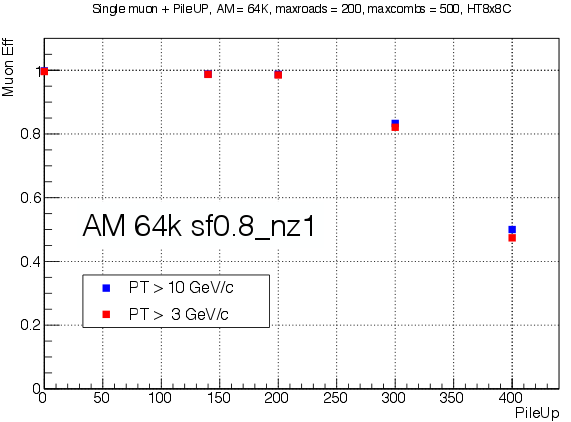
\includegraphics[width=4cm,height=4cm]{CMSL1TTfigs/luciano_mupu_sf0p8_plot}\\
		\item The author decided to check that and apply the $\Delta S$ approach (not considered by them at that time):\\
		\centering
		\includegraphics[scale=0.34]{CMSL1TTfigs/muon_road_eff_vs_pile_up_sf0p6}\\
		\includegraphics[scale=0.32]{CMSL1TTfigs/muon_road_eff_vs_pile_up_deltaS}
	\end{itemize}
	\end{multicols}	
\end{frame}

\begin{frame}{Simulation Studies: Stub Bending ($\Delta S$) - The Edge of the Montain}
	\vspace{-0.2cm}
	\begin{multicols}{2}
		\begin{itemize}
		\justifying
			\item At the ending of author's iteration with the CMS L1TT AM+FPGA there was a worry about PU spikes (as it happened in LHC Run I);
			\item Studies with single-$\mu$+PU presented in the group showed large efficiency loss at very high PU:\\
			\centering
			\begin{overpic}
				[width=4cm,height=4cm]{CMSL1TTfigs/luciano_mupu_sf0p8_plot}
				\put(20,0){
					\begin{overpic}[scale=0.2]{CMSL1TTfigs/surprised_cat}
					\put(45,20){\Huge \color{red} \textbf{$\Delta S$}}
					\put(25,9){\Huge \color{red} \textbf{MIRACLE!!}}
				\end{overpic}}
			\end{overpic}
			\item The author decided to check that and apply the $\Delta S$ approach (not considered by them at that time):\\
			\centering
			\includegraphics[scale=0.34]{CMSL1TTfigs/muon_road_eff_vs_pile_up_sf0p6}\\
			\includegraphics[scale=0.32]{CMSL1TTfigs/muon_road_eff_vs_pile_up_deltaS}	
		\end{itemize}		
	\end{multicols}	
\end{frame}

\begin{frame}{Simulation Studies: $\chi^{2}$ Revision}
	\begin{itemize}
		\justifying
		\begin{multicols}{2}		
			\item In order to optimize the final results, it was decided to re-study the tracking fitter $\chi^{2}$ value;
			\item It decides weather a combination of stubs is fine or not;
			\item Points to address:
			\begin{itemize}
		\justifying
				\item Just an unique cut applied;
				\item Dependence on the tracks $p_{T}$;
			\end{itemize}
			\flushright
			\begin{overpic}
				[scale=0.25]{CMSL1TTfigs/tfChi2_Pt_all}
			\end{overpic}
		\end{multicols}
		\item A new set of cuts have been adopted:
		\begin{itemize}
		\justifying
			\item 6/6 combinations have a tight and unique threshold given by the 99$\%$ percentile of the theoretical $\chi^{2}_{ndof=8}$ curve (equals to 20.2);
			\item 5/6 combinations have a $p_{T}$-based cut according to 8 ranges, which were defined to guarantee $\epsilon^{6/6+5/6}_{tracks} = 0.99 * \epsilon^{6/6+5/6}_{roads}$
		\end{itemize}
	\end{itemize}
\end{frame}

\begin{frame}{Simulation Studies: Synthetic Efficiency}
	\begin{itemize}
		\justifying
		\item Synthetic efficiency is meant to check the efficiency based on the track parameters ($q/p_{T}$, $\phi_{0}$, $z_{0}$ and $cot~\theta$);
		\item Task: match MC and AM reco tracks using their parameters;
		\item For so, one defines a $\chi^{2}$-like function:
		\begin{equation}
			\nonumber
			\chi^{2}_{match} = \sum_{i=0}^{4} \frac{\delta^{2}p_{i}}{\Omega^{2}(q/p_{T})_{i}}, 
			\quad
			\delta p_{i} = (p_{i}^{MC}-p_{i}^{Reco})
		\end{equation}
		\item The $\Omega$ function normalizes the dependence between the resolution in each track parameter and $q/p_{T}$:
	\end{itemize}
	\centering
	\begin{overpic}
		[scale=0.16]{CMSL1TTfigs/r_qbpT_fit_single_pion_nopu}
	\end{overpic}
	\begin{overpic}
		[scale=0.16]{CMSL1TTfigs/r_phi0_fit_single_pion_nopu}
	\end{overpic}
	\begin{overpic}
		[scale=0.16]{CMSL1TTfigs/r_z0_fit_single_pion_nopu}
	\end{overpic}
	\begin{overpic}
		[scale=0.16]{CMSL1TTfigs/r_cotTheta_fit_single_pion_nopu}
	\end{overpic}			
\end{frame}

\begin{frame}{Simulation Studies: Synthetic Efficiency}
	\begin{itemize}
		\justifying
		\item The $\chi_{match}$ establishes three types of tracks when receives a threshold value $\bar{q}$:
		\begin{itemize}
		\justifying
			\item \textbf{Good}: first reco track with smallest $\chi_{match}$ < $\bar{q}$;
			\item \textbf{Duplicate}: other reco tracks with $\chi_{match}$ < $\bar{q}$;
			\item \textbf{Fake}: any reco track with $\chi_{match}$ $\geq$ $\bar{q}$;
		\end{itemize}
		\item In order to define the value $\bar{q}$ a tracking match based on stubs and the synthetic efficiency were simultaneously done:
		\begin{itemize}
		\justifying
			\item Scanning the cut on $\chi_{match}$ one checks (on a dedicated MC sample) the number of original stubs composing the reco track;
			\item Then, one checks which cut reduces the Fake rate and increases the Good rate as much as possible and, avoiding random stub combinations (GOOD <5S);
			\item It was decided to have {\color{blue}$\chi_{match} = 40$};
		\end{itemize}
	\end{itemize}
	\centering
	\includegraphics[scale=0.35]{CMSL1TTfigs/jet250pu200_synthetic_view}
	\quad
	\includegraphics[scale=0.35]{CMSL1TTfigs/jet250pu200_analytic_view}	
\end{frame}	
	
\begin{frame}{Simulation Studies: Duplicate Removal}
	\begin{itemize}
		\justifying
		\begin{multicols}{2}
		\item The pattern match based on SS clusters produces several duplicate tracks in the CMS L1TT AM+FPGA;
		\item For that reason, a procedure to remove such tracks has been developed: the duplicate removal;\\
		\includegraphics[scale=0.2]{CMSL1TTfigs/tracks_duplication}
		\end{multicols}		
		\item The duplicate removal is a stub-based mechanism with the following algorithm:
		\begin{itemize}
		\justifying
			\item[1] A reco track is taken from the reco tracks list (\textbf{A}) and inserted on a new tracks list (\textbf{A});
			\item[2] Then, a loop is done over the remaining tracks on list \textbf{A}:
			\begin{itemize}
		\justifying
				\item If a track is found to share a given number $\bar{n}$ of stubs with any track on the list \textbf{B}, it is removed from list \textbf{A};
				\item Otherwise, the track is stored into the list \textbf{B};
			\end{itemize}
			\item[3] The tracks remaining in the list \textbf{B} are the final tracks;
		\end{itemize}
		\item The DR mechanism was studied in order to tune the minimum number of stubs which allows massive remotion of duplicated tracks and high synthetic efficiency;
	\end{itemize}
\end{frame}	

\begin{frame}{Simulation Studies: Duplicate Removal}
	\begin{itemize}
		\justifying
		\item Here are some results obtained for the DR tunning\footnote{\tiny Notice the gap between the track and synthetic efficiencies: that comes from the extra stubs which builds up a good (stubs) combination for the original track};
		\item The final DR cut was chosen to be 0 (zero);
	\end{itemize}
	\begin{table}
	\small
	\centering
	$\mu+PU200$\\
	\begin{tabular}{c|c|c|c|c|c}
		\hline
		\hline
		DR option & Goods & Duplicates & Fakes & Track eff & Synthetic eff\\
		\hline
		None      & 1.976 &	25.785	   & 0.614 & 0.985	   & 0.989\\
		5         & 1.976 &	25.785	   & 0.614 & 0.985	   & 0.989\\
		4         & 1.976 &	8.898	   & 0.275 & 0.98	   & 0.989\\
		3         & 1.973 &	0.604	   & 0.095 & 0.964	   & 0.989\\
		2         & 1.969 &	0.065	   & 0.047 & 0.953	   & 0.989\\
		1         & 1.967 &	0.007	   & 0.039 & 0.951	   & 0.988\\
		\rowcolor{light_red}
		0         & 1.966 &	0.000	   & 0.038 & 0.951	   & 0.988\\
		\hline
	\end{tabular}
	\\[0.2cm]
	$jet(p_{T}=250GeV)+PU200$\\
	\begin{tabular}{c|c|c|c|c|c}
		\hline
		\hline
		DR option & Goods & Duplicates & Fakes & Track eff & Synthetic eff\\
		\hline
		None	  & 8.506 &	143.735	   & 8.924 & 0.89	   & 0.897\\
		5	      & 8.506 &	143.735	   & 8.924 & 0.89	   & 0.897\\
		4	      & 8.506 &	52.935	   & 4.109 & 0.883	   & 0.897\\
		3	      & 8.481 &	4.746	   & 1.167 & 0.823	   & 0.895\\
		2	      & 8.431 &	0.642	   & 0.597 & 0.754	   & 0.889\\
		1	      & 8.412 &	0.067	   & 0.506 & 0.738	   & 0.887\\
		\rowcolor{light_red}
		0	      & 8.406 &	0.003	   & 0.482 & 0.74	   & 0.886\\
		\hline
	\end{tabular}
	\end{table}	
\end{frame}

\begin{frame}{Simulation Studies: Final FOMs}
	\begin{itemize}
		\justifying
		\item The next slides summarizes the final results found via the simulation package adopting the implementations presented here;
		\item The FOMs (figures of merit) are the common graphs used within the CMS L1TT AM+FPGA approach in order to show the performance of simulation studies;
		\item The FOMs are the efficiency and track categorization rates versus ($p_{T}$, $\eta$, $\phi$);
	\end{itemize}
\end{frame}

\begin{frame}{Simulation Studies: Final FOMs - $\mu$ in $t\bar{t}+PU200$}
	Track reconstruction efficiency for a $\mu$ in $t\bar{t}+PU200$ sample. The pattern bank used had 64k patterns and truncation at 200 roads and 500 combinations has been applied. Duplicate removal was applied by requiring DR=0.\\
	\begin{figure}
		\centering
		\begin{overpic}
			[scale=0.16,trim={1cm 0cm 1cm 1cm},clip]{CMSL1TTfigs/final_plots/ttbarPU200/ttbar_pu200_track_eff_pt_trunc}
		\end{overpic}
		\begin{overpic}
			[scale=0.16,trim={1cm 0cm 1cm 1cm},clip]{CMSL1TTfigs/final_plots/ttbarPU200/ttbar_pu200_track_eff_eta_trunc}
			\put(25,45){\color{blue}\tiny$\epsilon_{synthetic}(p_{T}>3GeV)$ = 0.80}
			\put(25,40){\color{red}\tiny$\epsilon_{synthetic}(p_{T}>3GeV)$ = 0.94}
			\put(25,35){\color{violet}\tiny$\epsilon_{synthetic}(p_{T}>3GeV)$ = 0.96}
		\end{overpic}
		\begin{overpic}
			[scale=0.16,trim={1cm 0cm 1cm 1cm},clip]{CMSL1TTfigs/final_plots/ttbarPU200/ttbar_pu200_track_eff_phi_trunc}
		\end{overpic}\\
		\begin{overpic}
			[scale=0.16,trim={1cm 0cm 1cm 1cm},clip]{CMSL1TTfigs/final_plots/ttbarPU200/ttbar_pu200_track_ratio_pt_trunc}
		\end{overpic}
		\begin{overpic}
			[scale=0.16,trim={1cm 0cm 1cm 1cm},clip]{CMSL1TTfigs/final_plots/ttbarPU200/ttbar_pu200_track_ratio_eta_trunc}
		\end{overpic}
		\begin{overpic}
			[scale=0.16,trim={1cm 0cm 1cm 1cm},clip]{CMSL1TTfigs/final_plots/ttbarPU200/ttbar_pu200_track_ratio_phi_trunc}
		\end{overpic}
	\end{figure}	
\end{frame}
	
\begin{frame}{Simulation Studies: Final FOMs - $\mu+PU200$}
	Track reconstruction efficiency for $\mu+PU200$ sample. The pattern bank used had 64k patterns and truncation at 200 roads and 500 combinations has been applied. Duplication removal was applied by requiring DR=0.
	\begin{figure}
		\centering
		\begin{overpic}
			[scale=0.16,trim={1cm 0cm 1cm 1cm},clip]{CMSL1TTfigs/final_plots/muPU200/mu_pu200_track_eff_pt_trunc}
		\end{overpic}
		\begin{overpic}
			[scale=0.16,trim={1cm 0cm 1cm 1cm},clip]{CMSL1TTfigs/final_plots/muPU200/mu_pu200_track_eff_eta_trunc}
			\put(25,45){\color{blue}\tiny$\epsilon_{synthetic}(p_{T}>3GeV)$ = 0.88}
			\put(25,40){\color{red}\tiny$\epsilon_{synthetic}(p_{T}>3GeV)$ = 0.97}
			\put(25,35){\color{violet}\tiny$\epsilon_{synthetic}(p_{T}>3GeV)$ = 0.98}
		\end{overpic}
		\begin{overpic}
			[scale=0.16,trim={1cm 0cm 1cm 1cm},clip]{CMSL1TTfigs/final_plots/muPU200/mu_pu200_track_eff_phi_trunc}
		\end{overpic}\\	
		\begin{overpic}
			[scale=0.16,trim={1cm 0cm 1cm 1cm},clip]{CMSL1TTfigs/final_plots/muPU200/mu_pu200_track_ratio_pt_trunc}
		\end{overpic}
		\begin{overpic}
			[scale=0.16,trim={1cm 0cm 1cm 1cm},clip]{CMSL1TTfigs/final_plots/muPU200/mu_pu200_track_ratio_eta_trunc}
		\end{overpic}	
		\begin{overpic}
			[scale=0.16,trim={1cm 0cm 1cm 1cm},clip]{CMSL1TTfigs/final_plots/muPU200/mu_pu200_track_ratio_phi_trunc}
		\end{overpic}	
	\end{figure}	
\end{frame}

\begin{frame}{Simulation Studies: Final FOMs - $\mu+PU300$}
	Track reconstruction efficiency for $\mu+PU300$ sample. The pattern bank used had 64k patterns and truncation at 200 roads and 500 combinations has been applied. Duplication removal was applied by requiring DR=0.
	\begin{figure}
		\centering
		\begin{overpic}
			[scale=0.16,trim={1cm 0cm 1cm 1cm},clip]{CMSL1TTfigs/final_plots/muPU300/mu_pu300_track_eff_pt_trunc}
		\end{overpic}
		\begin{overpic}
			[scale=0.16,trim={1cm 0cm 1cm 1cm},clip]{CMSL1TTfigs/final_plots/muPU300/mu_pu300_track_eff_eta_trunc}
			\put(25,65){\color{blue}\tiny$\epsilon_{synthetic}(p_{T}>3GeV)$ = 0.36}
			\put(25,60){\color{red}\tiny$\epsilon_{synthetic}(p_{T}>3GeV)$ = 0.95}
			\put(25,55){\color{violet}\tiny$\epsilon_{synthetic}(p_{T}>3GeV)$ = 0.94}
		\end{overpic}
		\begin{overpic}
			[scale=0.16,trim={1cm 0cm 1cm 1cm},clip]{CMSL1TTfigs/final_plots/muPU300/mu_pu300_track_eff_phi_trunc}
		\end{overpic}\\	
		\begin{overpic}
			[scale=0.16,trim={1cm 0cm 1cm 1cm},clip]{CMSL1TTfigs/final_plots/muPU300/mu_pu300_track_ratio_pt_trunc}
		\end{overpic}
		\begin{overpic}
			[scale=0.16,trim={1cm 0cm 1cm 1cm},clip]{CMSL1TTfigs/final_plots/muPU300/mu_pu300_track_ratio_eta_trunc}
		\end{overpic}	
		\begin{overpic}
			[scale=0.16,trim={1cm 0cm 1cm 1cm},clip]{CMSL1TTfigs/final_plots/muPU300/mu_pu300_track_ratio_phi_trunc}
		\end{overpic}	
	\end{figure}	
\end{frame}

\begin{frame}{Simulation Studies: Final FOMs - $\mu+PU400$}
	Track reconstruction efficiency for $\mu+PU400$ sample. The pattern bank used had 64k patterns and truncation at 200 roads and 500 combinations has been applied. Duplication removal was applied by requiring DR=0.	
	\begin{figure}
		\centering
		\begin{overpic}
			[scale=0.16,trim={1cm 0cm 1cm 1cm},clip]{CMSL1TTfigs/final_plots/muPU400/mu_pu400_track_eff_pt_trunc}
		\end{overpic}
		\begin{overpic}
			[scale=0.16,trim={1cm 0cm 1cm 1cm},clip]{CMSL1TTfigs/final_plots/muPU400/mu_pu400_track_eff_eta_trunc}
			\put(25,45){\color{blue}\tiny$\epsilon_{synthetic}(p_{T}>3GeV)$ = 0.36}
			\put(25,40){\color{red}\tiny$\epsilon_{synthetic}(p_{T}>3GeV)$ = 0.95}
			\put(25,35){\color{violet}\tiny$\epsilon_{synthetic}(p_{T}>3GeV)$ = 0.94}
		\end{overpic}
		\begin{overpic}
			[scale=0.16,trim={1cm 0cm 1cm 1cm},clip]{CMSL1TTfigs/final_plots/muPU400/mu_pu400_track_eff_phi_trunc}
		\end{overpic}\\	
		\begin{overpic}
			[scale=0.16,trim={1cm 0cm 1cm 1cm},clip]{CMSL1TTfigs/final_plots/muPU400/mu_pu400_track_ratio_pt_trunc}
		\end{overpic}
		\begin{overpic}
			[scale=0.16,trim={1cm 0cm 1cm 1cm},clip]{CMSL1TTfigs/final_plots/muPU400/mu_pu400_track_ratio_eta_trunc}
		\end{overpic}	
		\begin{overpic}
			[scale=0.16,trim={1cm 0cm 1cm 1cm},clip]{CMSL1TTfigs/final_plots/muPU400/mu_pu400_track_ratio_phi_trunc}
		\end{overpic}	
	\end{figure}	
\end{frame}
	
\begin{frame}{Simulation Studies: Final FOMs - $jets(p_{T}=250GeV)+PU200$}
	Track reconstruction efficiency for $jets(p_{T}=250GeV)+PU200$ sample. The pattern bank used had 64k patterns and truncation at 200 roads and 500 combinations has been applied. Duplication removal was applied by requiring DR=0.	
	\begin{figure}
		\centering
		\begin{overpic}
			[scale=0.16,trim={1cm 0cm 1cm 1cm},clip]{CMSL1TTfigs/final_plots/jet250PU200/jet250_pu200_track_eff_pt_trunc}
		\end{overpic}
		\begin{overpic}
			[scale=0.16,trim={1cm 0cm 1cm 1cm},clip]{CMSL1TTfigs/final_plots/jet250PU200/jet250_pu200_track_eff_eta_trunc}
			\put(25,50){\color{blue}\tiny$\epsilon_{synthetic}(p_{T}>3GeV)$ = 0.27}
			\put(25,45){\color{red}\tiny$\epsilon_{synthetic}(p_{T}>3GeV)$ = 0.78}
			\put(25,40){\color{violet}\tiny$\epsilon_{synthetic}(p_{T}>3GeV)$ = 0.71}		
		\end{overpic}
		\begin{overpic}
			[scale=0.16,trim={1cm 0cm 1cm 1cm},clip]{CMSL1TTfigs/final_plots/jet250PU200/jet250_pu200_track_eff_phi_trunc}
		\end{overpic}\\	
		\begin{overpic}
			[scale=0.16,trim={1cm 0cm 1cm 1cm},clip]{CMSL1TTfigs/final_plots/jet250PU200/jet250_pu200_track_ratio_pt_trunc}
		\end{overpic}
		\begin{overpic}
			[scale=0.16,trim={1cm 0cm 1cm 1cm},clip]{CMSL1TTfigs/final_plots/jet250PU200/jet250_pu200_track_ratio_eta_trunc}
		\end{overpic}	
		\begin{overpic}
			[scale=0.16,trim={1cm 0cm 1cm 1cm},clip]{CMSL1TTfigs/final_plots/jet250PU200/jet250_pu200_track_ratio_phi_trunc}
		\end{overpic}	
	\end{figure}
\end{frame}


\section{The Fast Matrix Element (FastME)}
\begin{frame}
	\center
	\begin{minipage}{10cm}
		\begin{varblock}[6.5cm]{}
			\center
			\huge \color{red} A Fast Matrix Element
		\end{varblock}
	\end{minipage}
\end{frame}

\subsection{Introduction}
\begin{frame}{Theoretical Foundation}
	\begin{itemize}
		\justifying
		\item Here is presented a procedure called \textit{Fast Matrix Element} (\textit{Fast}ME);
		\item It was studied in the very beginning of the author's PhD;
		\item The project was first idealized by prof(s). Andre Sznajder (DFNAE-UERJ) and Stephen Mrenna (CSD - FNAL):
		\begin{itemize}
		\justifying
			\item A method capable of deriving event weight from MC sampling into a given phase space;
			\item It should allow one to get proper normalization of random events, for instance;
		\end{itemize}
	\end{itemize}
	\begin{multicols}{2}
	\begin{varblock}[5.5cm]{\centering Why {\Huge Fast}?}
		\begin{table}
			Time to compute the weight per event via \textit{MadWeight}5. For an usual analysis these numbers multiply by thousand.\\
			\begin{tabular}{c|c}
				\hline
				Process                    & Time/Event (s)\\
				\hline
				ZH                         & $<$5\\
				$t\bar{t}$ fully-leptonic  &   10\\
				Zbb                        &   18\\
				$t\bar{t}$ semi-leptonic   &   41\\
				$t\bar{t}$H fully-leptonic &   60\\
				\hline
			\end{tabular}
		\end{table}		
	\end{varblock}
	\begin{varblock}[5.8cm]{\centering {\Huge ME} Methods}
	\begin{eqnarray}
		\nonumber
		\mathcal{P}(x|\alpha) &=& \frac{1}{\sigma_{\alpha}} \int d\omega_{1} d\omega_{2} f(\omega_{1}) f(\omega_{2})\\
		\nonumber
		&& \int d\Phi(y)|\mathcal{M}_{\alpha}(y)|^{2} W(x,y)
	\end{eqnarray}
	\vspace{-0.6cm}
	\begin{itemize}
		\justifying
		\item $\mathcal{P}(x|\alpha)$ is an event probability;
		\item $W(x,y)$ handled as approximation;
		\item $\mathcal{M}_{\alpha}(y)$ not possible for all physics;
		\item $\mathcal{M}_{\alpha}(y)$ in NLO or so on?
	\end{itemize}
	\end{varblock}
	\end{multicols}
\end{frame}

\begin{frame}{Theoretical Foundation}
	\begin{itemize}
		\justifying
		\item The original idea of finding event weights didn't lead to promising results: assigned weights didn't model properly the events;
		\item A new idea appeared, then: 
		\begin{itemize}
		\justifying
			\item Would it be possible to discriminate events based on a match between the particles from a probe event and a MC one?
		\end{itemize}
		\item \textit{Fast}ME algorithm:
		\begin{itemize}
		\justifying
			\item[1] Loop over the particles (i) from a MC event and match them to the particles (j) from a probe event according to
			\begin{equation}
				\nonumber
				R^{2}_{(i,j)} = \sum_{k=1}^{n}~ \left( \dfrac{v_{k}^{(i,MC)}-v_{k}^{(j,Data)}}{\sigma_{v_{k}}} \right)^2
			\end{equation}
			where, k stands for the kinematic variables ($p_{T}$, $\eta$, $\phi$) and the particles pairs $(i,j)$ are chosen to minimize $R_{i,j}$;
			\item[2] A distance between the probe event and the MC event is computed by summing in quadrature the minimum distances ($R_{i,j}$) between their particles:
			\begin{equation}
				\nonumber
				D^{2} = \sum_{i=1}^{m}~[R^{2}_{(i,j)}]_{min},~~\mathrm{with}~~j(i+1) ~!=~j(i)
			\end{equation}
			\item[3] Finally, a discriminant for the probe event is computed using the closest MC events (from each class) via the formulas
			\vspace{-0.5cm}
			\begin{multicols}{2}
				\begin{equation}
					\nonumber
					P_{SB}^{D} = \dfrac{D^{Bkg}_{Min}}{D^{Bkg}_{Min}+D^{Sig}_{Min}}
				\end{equation}\\
				\begin{equation}
					\nonumber
					P_{SB}^{W} = \dfrac{W^{Bkg}_{D_{min}}}{W^{Bkg}_{D_{min}}+W^{Sig}_{D_{min}}}
				\end{equation}
			\end{multicols}
		\end{itemize}
	\end{itemize}
\end{frame}

\begin{frame}{Theoretical Foundation}
	\begin{itemize}
		\justifying
		\item Here's an illustration of the method to clarify the algorithm. The MC events present a topology associated to the EM of a given physical process, such as, each particle has a correlation with the others particles in the event. An data event (black points) receives a probability of being from a kind or other (blue and red point) via the correlation of the distances (represented by the blue and red circles) between it and the MC events.
	\end{itemize}		
	\begin{figure}
	\flushleft
	\begin{overpic}
		[scale=0.4,trim={0cm 0cm 0cm 0cm},clip]{FastMEfigs/fastme_work_way}
		\put(60,77){\large $\phi$}
		\put(100,35){\large $\eta$}
		\put(66,29){{\color{red}$\bullet$}\hspace{0.07cm} class 1}
		\put(66,23){{\color{blue}$\bullet$}\hspace{0.07cm} class 2}
		\put(66,17){{\color{black}$\bullet$}\hspace{0.07cm} probe event}
		\put(65,10){{\color{red}$\bigcirc$} class 1 matches $[R^{2}_{(i,j)}]_{min}$}
		\put(65,2){{\color{blue}$\bigcirc$} class 2 matches $[R^{2}_{(i,j)}]_{min}$}
		\put(110,15){
			\begin{overpic}[scale=0.16]{FastMEfigs/psbD_vs_psbW}
				\put(5,71){\footnotesize $P_{SB}^{D} = \dfrac{D^{Bkg}_{Min}}{D^{Bkg}_{Min}+D^{Sig}_{Min}}$}
				\put(50,71){\footnotesize $P_{SB}^{W} = \dfrac{W^{Bkg}_{D_{min}}}{W^{Bkg}_{D_{min}}+W^{Sig}_{D_{min}}}$}
			\end{overpic}
		}
	\end{overpic}
	\end{figure}
\end{frame}

\subsection{Simulation Studies}
\begin{frame}{Simulation Studies: Bias from Pattern Bank Size}
	\begin{itemize}
		\justifying
		\item The first point addressed during the development of the project was the influence of the pattern banks size. On graphs (a) and (b) the background pattern bank has a fixed size while the signal one is varied. On graphs (c) and (d) the opposite case is shown. Note, here "purity" is computed using the absolute number of events (without normalization).
	\end{itemize}
	\begin{figure}
	\begin{overpic}
		[width=8cm,height=3cm,trim={0cm 0cm 0cm 0cm},clip]{FastMEfigs/purity_keeping_bkg_varying_sig}
		\put(25,20){(a)}
		\put(78,20){(b)}
	\end{overpic}\\[0.2cm]
	\begin{overpic}
		[width=8cm,height=3cm,trim={0cm 0cm 0cm 0cm},clip]{FastMEfigs/purity_keeping_sig_varying_bkg}
		\put(25,20){(c)}
		\put(78,20){(d)}		
	\end{overpic}
\end{figure}	
\end{frame}

\begin{frame}{Simulation Studies: Impact of $\phi$ Variable}
	\begin{itemize}
		\justifying
		\item Some studies have been done in order to optimize the performance of the discriminants;
		\item In the beginning of the project results showed that $\phi$ and $E$ (energy) doesn't contribute and can actually worse the discriminant performance;
		\item Below is a comparison between the $P_{SB}^{D}$ distribution using $\phi$ and without it:
		\begin{figure}
			\begin{overpic}
				[scale=0.2,trim={0cm 0cm 0cm 2.3cm},clip]{FastMEfigs/comparacao_psbD_using_nousing_dPhi_scaledPt70}
				\put(10,47){\color{red}Signal}
				\put(10,44){\color{blue}Background}		
			\end{overpic}
		\end{figure}			
		\item Based on such plot $\phi$ was removed from the default algorithm within $\textit{Fast}$ME and left as an option to the user;
	\end{itemize}
\end{frame}

\begin{frame}{Simulation Studies: Scaling $v_{k}$'s Contribution}
	\begin{itemize}
		\justifying
		\item Another point of optimization was the scaling of the variables used to compute the $R_{(i,j)}$;
		\item Since the variables $v_{k}$ present quite different ranges of variation it's important do level them;
		\item Here's a scan showing the variation of the fraction of signal events being mis-classified as background in function of the $\delta p_{T}$. A fixed value of $\delta \eta = 5.0$ was used;
		\begin{figure}
			\begin{overpic}
				[scale=0.2,trim={0cm 0cm 0cm 0cm},clip]{FastMEfigs/fastme_sensibility_vs_dpTscaleFactor}
			\end{overpic}
		\end{figure}
		\item The latest version of the project has an automated method which assigns the cumulative mean of MC events as the scaling factors;
	\end{itemize}
\end{frame}

\begin{frame}{Simulation Studies: \textit{Fast}ME Applied to HZZ4L CMS Data}
	\begin{itemize}
		\justifying
		\item After interesting results with MadGraph/Powheg/Sherpa samples of ggH and qqZZ, it was natural an interest of applying \textit{Fast}ME to the HZZ4L data collected by CMS on 2015 during the LHC RunI;
		\item The results have been compared to the formal CMS discriminant, the so called MELA for discriminating SM Higgs against $qqZZ$ background;
		\item Below: (a) observed events classified as signal and background by the \textit{Fast}ME, (b) $P_{SB}^{D}$ and (c) MELA discriminants distribution versus the $m_{4l}$.
	\end{itemize}
	\begin{figure}
	\centering
	\begin{overpic}
		[width=3.8cm,height=4cm,trim={0cm 0cm 13cm 0cm},clip]{FastMEfigs/fastme_discriminant_and_m4l}
		\put(45,-8){(a)}
	\end{overpic}
	\begin{overpic}
		[width=3.8cm,height=3.8cm,trim={0cm 0cm 11.4cm 0cm},clip]{FastMEfigs/fastme_2D_m4l_comparison_to_mela}
		\put(50,-8){(b)}
	\end{overpic}
	\begin{overpic}
		[width=3.8cm,height=3.8cm,trim={11.6cm 0cm 0cm 0cm},clip]{FastMEfigs/fastme_2D_m4l_comparison_to_mela}
		\put(50,-8){(c)}
	\end{overpic}	
	\end{figure}	
\end{frame}

\subsection{The FastME Package}
\begin{frame}{The \textit{Fast}ME Package}
	\begin{itemize}
		\justifying
		\item The success of \textit{Fast}ME idea on real CMS data encouraged us to move the standalone codes created until that moment into a organized package;
		\item During the author's first travel to Fermilab, this package started to be maintained on GitHub:
	\end{itemize}
	\centering
	\includegraphics[scale=0.34]{FastMEfigs/fastme_github_page}	
\end{frame}

\begin{frame}{The \textit{Fast}ME Package}
	\begin{multicols}{2}
	\begin{itemize}
		\justifying
		\item Features:
		\begin{itemize}
			\begin{minipage}{5cm}
			\item User gives to the program a configuration file;
			\item Original samples are replicated;
			\item $R_{(j,i)}$ can be simultaneously computed for each class;
			\item Creates a ROOT file containing $D_{min}^{class}$ and $P_{SB}^{D/W}$;
			\end{minipage}			
		\end{itemize}
	\end{itemize}
	\centering
	\begin{overpic}
		[scale=0.4,trim={0cm 4.1cm 0cm 7cm},clip]{FastMEfigs/fme_config_card}
		\put(0,43){\scriptsize \textit{Fast}ME configuration file example}
	\end{overpic}
	\begin{overpic}
		[scale=0.2,trim={0cm 25cm 0cm 0cm},clip]{FastMEfigs/fme_running}
		\put(0,101){\scriptsize \textit{Fast}ME workflow view}
	\end{overpic}\\:\\
	\begin{overpic}
		[scale=0.2,trim={0cm 0cm 0cm 40cm},clip]{FastMEfigs/fme_running}
		\put(76,60){\includegraphics[scale=0.11]{FastMEfigs/Discriminant_Signal_vs_Background}}
		\put(76,0){\includegraphics[scale=0.11]{FastMEfigs/FastMatrixElement_ROC_Curve}}
	\end{overpic}
	\end{multicols}	
\end{frame}

\begin{frame}{The End of \textit{Fast}ME Project}
	\begin{itemize}
		\item Although the modified original idea of \textit{Fast}ME has showed some nice results we faced two issues:
		\begin{itemize}
			\item It doesn't have a good performance for discriminating VBF against ggH;
			\item TMVA has a similar implementation and is more flexible;
		\end{itemize}		
		\includegraphics[width=5cm,height=5cm,trim={0cm 0cm 18cm 0cm},clip]{FastMEfigs/ggH_vs_VBF_test}
		\quad
		\includegraphics[width=6cm,height=4.5cm,trim={0cm 0cm 0cm 0cm},clip]{FastMEfigs/knn_tmva}
		\item Such issues lead to the end of the project:
		\begin{itemize}
			\item No power enough for the presented physics analysis;
			\item Not a new method (we re-invented the wheel);
		\end{itemize}
	\end{itemize}
\end{frame}

\section{Conclusions}
\begin{frame}
	\center
	\begin{minipage}{10cm}
		\begin{varblock}[5cm]{}
			\center
			\huge \color{red} CONCLUSIONS %\\ AND\\ FUTURE PLANS
		\end{varblock}
	\end{minipage}
\end{frame}


\begin{frame}{Conclusions: CMS-AN-18-120}
	\begin{itemize}
		\justifying
		\item {\color{blue}ANN approach successfully implemented for an isolated VBF $H \rightarrow ZZ \rightarrow 4l$ XS measurement};
		\item {\color{blue}Reliable} procedure implemented for {\color{blue}systematic uncertainties};
		\item {\color{blue}Results} provided from the combination of our {\color{blue}best ANN configurations}:
		\begin{itemize}
		\justifying
			\item best fit for signal strength: {\color{blue}$\mu_{qqH}^{Exp} = 1.00_{-0.70}^{+1.08}$} and {\color{blue}$\mu_{qqH}^{Obs} = 1.28_{-0.84}^{+1.24}$};
			\item 95$\%$CL upper limits on $\mu_{qqH}$: {\color{blue}$\mu_{qqH}^{Exp} < 1.66$} and {\color{blue}$\mu_{qqH}^{Obs} < 3.79$};
			\item significances: {\color{blue}$\sigma_{qqH}^{Exp} = 1.8$} and {\color{blue}$\sigma_{qqH}^{Obs} = 1.9$};
		\end{itemize}
		\item {\color{blue}Projections} provided for future luminosity scenarios at the LHC:
		\begin{itemize}
		\justifying
			\item Expected to improve signal strength precision up to {\color{blue}$\sim$87$\%$} at the end of RunII;
			\item Significance evolution:\\
			\begin{tabular}{c|c|c|c|c|c|c|c}
				\hline
				Luminosity (fb$^{-1}$) & 35.9 & 150.0 & 300.0 & 359.0 & 1077.0 & 1795.0 & 3000.0\\
				\hline
				Factor                 & 1.00 & 4.18  & 8.36  & 10.00 & 30.00  & 50.00  & 83.57\\
				\hline
				Expected significance  & 1.8  & 3.4   & 4.7   & 5.1   & 8.6    & 10.9   & 14.0\\
				\hline
			\end{tabular}
		\end{itemize}
		\item Analysis documentation is ready and released: {\color{blue}AN-18-120};
		\item {\color{blue}No issues} raised last meeting with HZZ subgroup (December 7$^{th}$, 2018) at CERN (green light for a thesis endorsement);
	\end{itemize}
\end{frame}

\begin{frame}{Conclusions: CMS-AN-18-120}
	\begin{itemize}
		\justifying
		\item {\color{red}Ongoing}: analysis of full {\color{blue}2017 MC $\&$ Data}:
		\begin{itemize}
		\justifying
			\item package of macros for future studies (parallel ANN training, Z+X derivation and statistical analysis);
			\item already in use by a colleague in Bari (Nicola's student).
		\end{itemize}
	\end{itemize}
	\centering
	\includegraphics[scale=0.45]{figs/github_AN_18_120}
\end{frame}

\begin{frame}{Conclusions: CMS L1TT AM+FPGA}
	\begin{itemize}
		\item Significant contribution has been given to the CMS L1TT AM+FPGA:
		\begin{itemize}
			\item Several new MC samples generated and made available for the group;
			\item Developments, studies and implementations:
			\begin{itemize}
				\item Synthetic matching and efficiency;
				\item Duplicate removal;
				\item Stub bending ($\Delta S$);
				\item Effects of truncation on roads and/or combinations;
				\item Tracking fitter $\chi^{2}$ cut revision;
			\end{itemize}
			\item Support during the electronic inspection:
			\begin{itemize}
				\item Check up of Pulsar BII boards and the PRMs;
				\item Check up of optical cables connecting Pulsar boards;
				\item Check up of boards connected in the crates;
			\end{itemize}
			\item Creation of a dedicated documentation explaining some of the nomenclature adopted in the approach, detailing some workflow and implementations developed within the package;
		\end{itemize}
	\end{itemize}
\end{frame}
		
\begin{frame}
	\begin{center}
		\includegraphics[scale=0.5]{figs/backup}
	\end{center}
\end{frame}

\begin{frame}{Datasets used in the Analysis}
	\centering
	\includegraphics[scale=0.5,trim={0cm 0.5cm 0cm 0cm},clip]{figs/datasets}
\end{frame}

\begin{frame}{JETMET POG Filters}
	\centering
	\includegraphics[scale=0.6,trim={0cm 0cm 0cm 0.5cm},clip]{figs/met_filters}
\end{frame}

\begin{frame}{Post-Fit Yields and Distributions}
	\centering
	\includegraphics[scale=0.45]{figs/postfit_yields}\\[0.2cm]
	\includegraphics[scale=0.5]{figs/postfit_shapes}
\end{frame}

\begin{frame}{Comparison Between Best Fits of Njets2 and Njets3 Categories}
	\begin{itemize}
		\justifying
		\item The best fits from each jet-based category. As it is shown, there's no advantage in using them alone instead of combining as it was done in the analysis;
	\end{itemize}
	\centering
	\includegraphics[scale=0.25]{figs/ChannelCompatibility_ComparisonBetweenNjets2Njets3}
\end{frame}

\begin{frame}{Sensitivity of Combined ANNs}
	\begin{itemize}
		\justifying
		\item Note that, no systematic uncertainty has been accounted here;
	\end{itemize}
	\centering
	\includegraphics[scale=0.7,trim={2cm 9.5cm 2cm 0cm},clip]{figs/ann_comb_sensitivity}
	\includegraphics[scale=0.7,trim={2cm 1cm 2cm 8.6cm},clip]{figs/ann_comb_sensitivity}
\end{frame}

\begin{frame}{ANNs Validation Plots}
	\centering
	\includegraphics[scale=0.7,trim={0cm 11.7cm 0cm 0cm},clip]{figs/ann_validation_plots}
	\includegraphics[scale=0.7,trim={0cm 6cm 5.4cm 5.8cm},clip]{figs/ann_validation_plots}\\[0.5cm]
	\includegraphics[scale=0.7,trim={5.4cm 6cm 0cm 5.8cm},clip]{figs/ann_validation_plots}
	\includegraphics[scale=0.75,trim={0cm 0cm 0cm 11.5cm},clip]{figs/ann_validation_plots}
\end{frame}

\begin{frame}{Events after SM Higgs Selections in each 4l Channel}
	\centering
	\includegraphics[scale=0.5]{figs/smhiggs_m4l_channels}
\end{frame}

\begin{frame}{Z+X Systematic Uncertainty and Final Yields}
	\begin{itemize}
		\justifying
		\item Z+X systematic uncertainty from FR: compute its variation by averaging MC ($D\varUpsilon$, $ZZ/Z\gamma$, $WZ$, $t\bar{t}$) FR and reweighing with 2P2F yields. Then propagate to Z+X estimation;
	\end{itemize}
	\centering
	\includegraphics[scale=0.7,trim={0cm 1.5cm 0cm 0cm},clip]{figs/FR_average_and_reweight_1D}
\end{frame}

\begin{frame}{Z+X Systematic Uncertainty and Final Yields}
	\begin{itemize}
		\justifying
		\item The behavior in 2D:
	\end{itemize}
	\centering
	\includegraphics[scale=0.6]{figs/FR_average_and_reweight}
\end{frame}

\begin{frame}{Z+X Systematic Uncertainty and Final Yields}
	\centering
	\includegraphics[scale=0.7]{figs/zx_final_yields}
\end{frame}

\begin{frame}{Systematic Uncertainties Impact on $\mu_{qqH}$ Fit}
	\centering
	\includegraphics[scale=0.5]{figs/impacts_obs_4l_combination}
\end{frame}

\begin{frame}{Architecture of Chosen ANNs}
\begin{figure}
	\caption{ANNs architecture created in this analysis. Black dots stand for inputs/neurons, while lines stand for the size of the ANN parameters chosen after training them. Wider and brighter lines means the parameter (weight or bias) associated to a given input for a neuron is larger (in other words its contribution is more relevant). ANN for Njets2 has 21:13:8 hidden neurons, while for Njets3 it has 11:9:7 (all neurons of SeLU type).}
	\subfloat[Njets2 - 21:13:8]{\includegraphics[width=6cm,height=5cm]{figs/k57nj2_architecture_horizontal}}
	\subfloat[Njets3 - 11:9:7]{\includegraphics[width=6cm,height=5cm]{figs/k24nj3_architecture_horizontal}}
\end{figure}
\end{frame}

%-------------------------------------------------------------
\end{document}
